%Carattere dimensione 12
\documentclass[12pt]{report}

%Margini e interlinea
\usepackage[top=1in, bottom=1in, left=1.4in, right=1in]{geometry}
\usepackage{tcolorbox}
\usepackage{url}
\urlstyle{same}
\pagestyle{plain}
\linespread{1.3}

%Librerie utili
\usepackage{afterpage}
\usepackage[italian]{babel}
\usepackage[utf8]{inputenc}
\usepackage{libertine}
\usepackage{graphicx}
\usepackage{floatflt}
\usepackage{blindtext}
\usepackage{enumitem}
\usepackage{amsthm}
\usepackage{subfig}
\usepackage{listings}
\usepackage{listingsutf8}
\usepackage{amsmath}
\usepackage{framed}
\usepackage{minibox}
\usepackage{float}
\usepackage{wrapfig}
\usepackage{longtable}
\usepackage[strict]{changepage}
\usepackage{pgfplots}
\usepackage{tikz}
\usetikzlibrary{matrix}
\pgfplotsset{width=11cm,compat=1.9}
\usepgfplotslibrary{external}
\usepackage{hyperref}
\hypersetup{
    colorlinks,
    citecolor=black,
    filecolor=black,
    linkcolor=black,
    urlcolor=black
}


\tikzexternalize

\begin{document}

\begin{titlepage}
\begin{figure}[t]
	\centering
\includegraphics[width=0.9\textwidth]{scritta}
    \centering
\includegraphics[width=0.4\textwidth]{logo}
\end{figure}

\begin{center}
	\textbf{ Dipartimento di Informatica\\ Corso di Laurea in Informatica\\}
	\vspace{15mm}
    {\LARGE{\bf Costruzione ed analisi del grafo delle transazioni di Ethereum}}\\
	\vspace{3mm}
	
\end{center}

\vspace{36mm}

\begin{minipage}[t]{0.52\textwidth}\raggedright
	{\large{\bf Relatori:\\ Prof.ssa Laura Ricci\\Dott. Damiano Di Francesco Maesa} }
\end{minipage}\hfill\begin{minipage}[t]{0.30\textwidth}\raggedleft
	{\large{\bf Candidato: \\ Luca Corbucci\\ }}
\end{minipage}

\vspace{18mm}

\centering{\large{\bf Anno Accademico 2017/2018 }}

\end{titlepage}

\newpage\null\thispagestyle{empty}\newpage

\tableofcontents

\chapter{Introduzione}
\fontsize{13pt}{15pt}\selectfont

Nel 2008 Satoshi Nakamoto presentava al mondo Bitcoin descrivendone il funzionamento nel paper 'Bitcoin: A Peer-to-Peer Electronic Cash System' \cite{BitcoinWhitePaper}.
L'obiettivo di Bitcoin era quello di utilizzare una rete peer-to-peer per lo scambio di denaro digitale sfruttando una tecnologia denominata Blockchain. 
Nella blockchain i dati vengono memorizzati all'interno di blocchi contenenti, nel caso di Bitcoin, le transazioni svolte tra i vari nodi della rete.
Ogni utente che vuole entrare nella rete peer-to-peer di Bitcoin e svolgere una transazione ha solo bisogno di essere in possesso di un  indirizzo di 160 bit che lo possa identificare univocamente.
\newline
Ciò che garantisce la sicurezza della blockchain è il legame tra i vari blocchi, per ognuno di essi viene calcolato un hash che dipende anche dall'hash del blocco precedente.
Ogni blocco è quindi dipendente da tutti i predecessori e si crea una catena che rende praticamente impossibile la modifica dei dati contenuti all'interno della blockchain a causa dell'alta potenza computazionale che sarebbe richiesta.

Alla fine del 2013 Vitalik Buterin ha presentato Ethereum, che rappresenta una evoluzione della blockchain di Bitcoin.
\newline 
Così come Bitcoin, anche Etherum sfrutta la blockchain per il salvataggio delle informazioni delle transazioni, la principale novità è l'introduzione degli smart contracts.
Nella blockchain di Ethereum è infatti possibile memorizzare anche del codice che viene poi eseguito grazie alla virtual machine decentralizzata chiamata Ethereum Virtual Machine (EVM).
La presenza della EVM permette di scrivere del codice tramite un linguaggio Turing Completo e di eseguire il bytecode sui vari nodi della rete. Questo codice che viene eseguito prende il nome di smart contract e può essere scritto con vari linguaggi di programmazione, tra cui Solidity.
\newline
Gli smart contract vivono sotto forma di bytecode distribuito sui vari nodi che compongono la rete peer-to-peer di Ethereum e grazie all'innovazione introdotta, sono stati la chiave del successo di Ethereum.
I miner della rete utilizzano la EVM per eseguire il bytecode del contratto, una volta terminata l'esecuzione sarà possibile inserire la transazione di chiamata del contratto in un blocco nella blockchain solo se tutti i nodi raggiugono il consenso.
Qualsiasi utente può creare un nuovo smart contract pagando una quantità di ether proporzionata alla dimensione occupata dal bytecode del contratto.


Sia le transazioni contenute nella blockchain di Bitcoin che di Ethereum si prestano ad essere rappresentate in un grafo.
Nel caso di Ethereum, all'interno del grafo ogni nodo corrisponderà ad un indirizzo mentre ogni arco ad una transazione.
Una volta ottenuta la rappresentazione mediante un grafo di tutte le transazioni, è utile svolgere delle analisi cercando di comprendere le caratteristiche più interessanti e particolari della rete.
\newline
Questa analisi è già stata svolta per la blockchain di Bitcoin e durante il tirocinio l'obiettivo è stato quello di effettuare lo stesso insieme di analisi anche con Ethereum.
I risultati delle analisi svolte sulla blockchain di Bitcoin sono stati pubblicati in vari paper \cite{maesa2016uncovering} \cite{maesa2016analysis} \cite{maesa2017data} \cite{maesa2017detecting}
e hanno fornito una conoscenza più approfondita della rete peer to peer di Bitcoin.


Il tirocinio è iniziato con una fase di studio del protocollo di Ethereum e della sua blockchain. 
In particolare dovendo produrre un parser delle transazioni, era necessario conoscere nel dettaglio la struttura interna dei blocchi contenuti nella blockchain, delle transazioni e dei transaction receipt.
La conoscenza di questi argomenti piuttosto tecnici è stata approfondita mediante la lettura dei paper pubblicati dagli sviluppatori di Ethereum \cite{YellowPaper}.
\newline
Dopo aver compreso queste informazioni è stato possibile passare alla parte operativa del lavoro che ha comportato la scrittura di un parser in Java che, dato in input un file esadecimale contenente tutte le transazioni suddivise in blocchi, potesse restituire per ogni transazione gli indirizzi di mittente e destinatario, il timestamp e lo status della transazione.
Durante lo sviluppo del parser però si sono presentate alcune problematiche che inizialmente non erano state considerate:

\begin{itemize}
    \item Con i dati che avevamo a disposizione non era possibile comprendere se una transazione fosse fallita o meno durante l'esecuzione;
    \item Recuperare l'indirizzo del mittente di una transazione richiedeva dei calcoli abbastanza complicati che avrebbero aumentato di molto il tempo necessario al parsing di tutti i dati.
    \item Con le transazioni utilizzate per la creazione di nuovi contratti ci siamo scontrati con una problematica simile a quella appena descritta, anche in questo caso il calcolo dell'indirizzo del contratto appena creato avrebbe richiesto calcoli complicati.
\end{itemize}

Considerate queste problematiche abbiamo pensato ad un secondo approccio al problema.
Abbiamo creato un nodo ed eseguito la sincronizzazione della blockchain di Ethereum e poi utilizzato Geth \cite{goEthereum} per estrarre tutte le informazioni necessarie direttamente dalla blockchain.
Questa soluzione ha richiesto la scrittura di alcuni script in Javascript e si è rivelata efficace dato che ci ha permesso di recuperare i dati della blockchain, compreso lo status delle transazioni che con il parser in Java non eravamo riusciti a ricavare.
\newline
Anche questa soluzione ha comunque un alto costo computazionale per l'estrazione ed il parsing dei dati della blockchain.

Una volta ottenuto un dataset significativo abbiamo utilizzato WebGraph \cite{WebGraph} per la creazione del grafo e per svolgere le analisi.
Visto il tipo di dati in nostro possesso, non ci siamo limitati a svolgere l'analisi solamente sul grafo completo con tutte le transazioni ma abbiamo suddiviso il dataset prima in base al tipo di transazione e poi in base al timestamp dei blocchi.

Il grafo completo contiene tutte le transazioni comprese tra il blocco 0 e il 4237648, sono presenti al suo interno 6081755 nodi e 7224840 archi.
I nodi rappresentano i vari indirizzi della rete ethereum mentre gli archi le transazioni.
L'analisi svolta su questo grafo ci ha restituito i seguenti risultati:
\begin{itemize}
    \item Il diametro del grafo in questione ha una lunghezza di 8267 nodi con una distanza media tra i nodi di 4.33;
    \item L'enorme differenza che troviamo tra la lunghezza del diametro e la distanza media ci ha fatto pensare che possano essere presenti all'interno del grafo dei cammini ``artificiali`` anomali;
    \item Abbiamo calcolato il grado entrante ed uscente dai vari nodi della rete producendo un grafico delle distribuzioni.
    Il risultato ottenuto mostra in entrambi i casi un comportamento di tipo power law, questo indica che nel grafo sono presenti molti account che ricevono o inviano poche transazioni e poi un numero limitato di indirizzi che ne ricevono o inviano molte;
    \item Abbiamo svolto l'analisi della centralità del grafo basandoci sul grado entrante ed uscente dei nodi. Successivamente è stata calcolata anche la centralità armonica.
    Confrontando i risultati ottenuti con queste due analisi abbiamo notato che molti nodi compaiono in entrambi le ``classifiche``. 
    Questo risultato ci ha fornito una panoramica degli account più importanti per la rete Ethereum, in particolare abbiamo notato che molti di essi sono riconducibili a degli exchange.
\end{itemize}


I risultati che abbiamo trovato più interessanti sono quelli ottenuti grazie all'analisi temporale. 
Il dataset è stato suddiviso in 17 snapshot e su ognuno sono state svolte delle analisi che ci hanno permesso una migliore comprensione dell'evoluzione della rete di Ethereum nel corso del tempo.
Questa fase di analisi ha restituito i seguenti risultati:

\begin{itemize}
    \item Il numero di nodi e transazioni è cresciuto in modo evidente nel periodo compreso tra Marzo e Settembre 2017 quando da circa 1 milione di nodi si è passati a più di 6 milioni.
    Questa crescita è probabilmente legata all'aumento del valore dell'Ether.
    \item Per ogni snapshot è stata calcolata la lunghezza del diametro del grafo, questa, dopo un periodo iniziale in cui si mantiene costante, assume improvvisamente un valore superiore a 8000.
    La lunghezza del diametro rimane poi costante in tutti gli snapshot successivi ad esclusione del periodo compreso tra Aprile e Giugno 2016 quando diminuisce fino a 5000 nodi.
    Questa diminuzione della lunghezza del diametro si ripercuote anche sulla distanza media tra i nodi del grafo, nello stesso periodo infatti si verifica anche una diminuzione di questo valore.
    \item Avendo a disposizione lo studio della centralità sulla base del grado entrante ed uscente, per ogni snapshot è stato possibile generare una ``classifica`` di nodi più attivi. 
    In particolare abbiamo analizzato la storia e il balance relativo agli account che maggiormente sono rimasti nella classifica dei più attivi. Tra i risultati più interessanti ci sono quelli relativi ad account che sono stati vittime di attacchi hacker.
    \item Studiando tramite gli snapshot l'evoluzione della dimensione della componente connessa più grande, abbiamo notato che oltre il 90\% dei nodi sono sempre presenti all'interno di questo sottografo. 
\end{itemize}

L'ultima analisi è stata svolta sui grafi suddivisi in base al tipo di transazioni. Abbiamo prodotto un grafo con le sole transazioni tra utenti esterni, uno con quelle verso i contratti e uno con le sole richieste di creazione di nuovi smart contracts ottenendo i seguenti risultati:

\begin{itemize}
    \item Dividendo il dataset ci siamo resi conto che l'80.4\% delle transazioni della blockchain vengono inviate da utenti esterni ad altri utenti esterni. Le transazioni verso contratti rappresentano il 15.5\% del totale e solamente il 4\% sono utilizzate per creare nuovi contratti.
    \item Abbiamo studiato la distribuzione del grado uscente all'interno del grafo con le sole transazioni utilizzate per la creazione di contratti. Il risultato ottenuto mostra un comportamento di tipo power law con tanti nodi che creano pochi contratti e pochi nodi che ne creano molti.
    \item Nel grafo con le sole transazioni verso contratti è stata studiata la distribuzione del grado entrante per comprendere quante chiamate ricevono gli smart contracts. 
    Anche in questo caso nel grafico abbiamo ottenuto una power law.
    \item Sia per il grafo con le sole transazioni verso contratti sia per quello con le richieste di creazione di nuovi smart contracts è stata studiata la centralità in base al grado entrante.
    Questa analisi ci ha permesso di comprendere quali sono i contratti che hanno ricevuto il maggior numero di chiamate e chi sono gli utenti esterni che hanno creato più smart contracts.
    
\end{itemize}

La relazione è strutturata come segue:

\begin{itemize}
    \item Capitolo 2: in questo capitolo si si illustrano le principali caratteristiche di Bitcoin, di Ethereum e della tecnologia Blockchain;
    \item Capitolo 3: in questa sezione vengono descritte le analisi più comuni che possono essere svolte su un grafo di grandi dimensioni come quello contentente le transazioni di Ethereum;
    \item Capitolo 4: in questo capitolo è riportata la descrizione dei vari strumenti che sono stati utilizzati durante il tirocinio;
    \item Capitolo 5: in questo capitolo vengono presentate alcune caratteristiche tecniche di Ethereum descrivendo la struttura di blocchi, transazioni e transaction receipt, viene inoltre data una descrizione dei Patricia Merkle Tree.
    \newline Si descrive il lavoro svolto durante il tirocinio e i due parser utilizzabili per l'estrazione dei dati dalla blockchain Ethereum;
    \item Capitolo 6: questo capitolo tratta della parte finale del tirocinio ovvero l'analisi del grafo e i risultati ottenuti;
    \item Capitolo 7: vengono riportate le conclusioni ed un'analisi degli sviluppi futuri.
\end{itemize}

\chapter{Background}

In questo capitolo viene descritta la storia delle cryptocurrencies e la nascita della tecnologia blockchain con le sue possibili applicazioni.
Ci focalizzeremo in particolare su Bitcoin spiegando in che modo l'utilizzo della Blockchain lo rende sicuro. 
Successivamente verranno anche descritte le principali caratteristiche di Ethereum e le sue principali differenze con Bitcoin.

\section{Storia delle cryptocurrencies e nascita della tecnologia blockchain}

Nel corso della storia l'uomo ha sempre avuto la necessità di scambiarsi dei beni e questo ha portato alla nascita di varie forme di pagamento, la più antica è stata il baratto, poi l'uomo si è evoluto ed è nata la carta moneta che ancora oggi utilizziamo.
\newline Il commercio negli ultimi anni si è spostato sempre di più verso internet, dove viene gestito da istituzioni finanziarie che vengono utilizzate come garanti per i pagamenti elettronici e non è possibile svolgere una transazione senza fare riferimento ad un intermediario.
\newline Il problema dei pagamenti elettronici è la possibilità che questi siano, in alcuni casi, reversibili, questo comporta una minore fiducia nei confronti del cliente che vuole acquistare un bene da un qualsiasi negozio online.
Inoltre anche il proprietario del negozio potrebbe ricevere dal cliente il compenso stabilito senza poi spedire quello che è stato acquistato.
I problemi legati ai pagamenti e soprattutto la volontà di creare un sistema che non prevedesse una terza parte in una transazione tra due utenti hanno portato alla nascita di nuove valute che, a differenza delle precedenti, sono virtuali e basate su prove crittografiche, prendono il nome di cryptocurrencies.
L'idea delle cryptocurrencies è più vecchia di quanto si possa pensare, già nel 1992 un gruppo di persone si riunirono in una mailing list denominata Cypherpunk \cite{Cypherpunk} in cui si affrontava questo argomento.
\newline
La svolta nel mondo delle cryptocurrencies si ebbe però il 31 Ottobre 2008 quando Satoshi Nakamoto annunciò nella mailing list ``Cryptography`` la disponibilità di un paper di 8 pagine destinato a riscrivere la storia delle cripto valute: ‘Bitcoin: A Peer-to-Peer Electronic Cash System' \cite{BitcoinWhitePaper}.
\newline Il, o i creatori di Bitcoin sono riusciti a creare una moneta decentralizzata e un sistema che, nonostante utilizzi una rete peer-to-peer, riesce ad evitare il problema del double-spending senza avere la necessità di una terza parte che controlli le transazioni.
\newline Con il termine ``double-spending`` intendiamo il problema per cui una singola moneta virtuale può essere spesa più di una volta dallo stesso utente.
Per risolvere il problema del double spending le transazioni di Bitcoin sono pubbliche, in questo sistema è centrale il ruolo del miner che ha il compito di garantire tutte le transazioni in modo che il beneficiario possa essere sicuro che il mittente non abbia già speso i soldi che gli sta inviando.
La grande novità introdotta da Bitcoin è rappresentata dalla struttura totalmente decentralizzata utilizzata per memorizzare le transazioni degli utenti, questa è stata chiamata Blockchain, tutte le informazioni sono salvate su migliaia di nodi e non in un solo server.
All'interno della blockchain le informazioni sono suddivise in blocchi legati tra di loro.

\begin{figure}[H]
    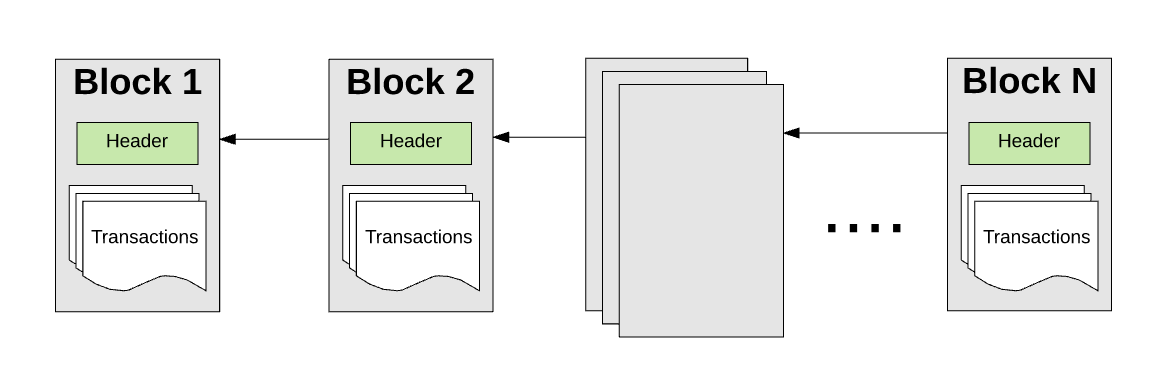
\includegraphics[width=\textwidth]{Blocks}
    \caption{Ogni blocco è legato dall'hash del precedente}
\end{figure}

Per implementare questo sistema di conferma delle transazioni e di creazione dei blocchi viene utilizzato un algoritmo Proof-of-Work denominato Hashcash che incentiva i miner a competere tra loro nella produzione dei blocchi e garantisce anche una protezione dagli attacchi Sybil.
I miner della rete Bitcoin, per creare un blocco da inserire nella blockchain, devono risolvere problemi matematici molto complessi che richiedono un'alta potenza computazionale ma che allo stesso tempo permettano una rapida verifica della soluzione.
La difficoltà dei problemi da risolvere varia in base alla potenza di calcolo disponibile nella rete. La richiesta di una potenza sempre maggiore ha messo in luce un lato negativo della Proof of Work, l'eccessivo consumo di energia elettrica e la necessità di disporre di macchine altamente specializzate.

Tutto questo sistema garantisce sicurezza alla blockchain e alle transazioni Bitcoin perchè per modificare una vecchia transazione presente nel blocco N e andare quindi a spendere di nuovo la stessa quantità di moneta dovremmo modificare anche tutti i blocchi successivi, operazione praticamente impossibile a causa della potenza computazionale richiesta.


\section{Ethereum}

Una delle più interessanti applicazioni della blockchain è rappresentata da Ethereum.
\newline
Ethereum è una piattaforma basata sulla blockchain che ha l'obiettivo di permettere agli utilizzatori l'esecuzione di ``smart contracts``, è stata sviluppata da Vitalik Buterin che l'ha presentata in un paper pubblicato nel Dicembre 2013 \cite{ethereumWhitePaper}.
Uno Smart Contract è la “traduzione” in codice di un contratto capace di verificare in automatico l’avverarsi di determinate condizioni e di eseguire delle azioni nel momento in cui le condizioni decise tra le parti sono raggiunte e verificate.
Per la creazione degli smart contract Ethereum mette a disposizione vari linguaggi di programmazione Turing Completi come Solidity o Serpent.

Attualmente anche Ethereum utilizza la Proof of Work come algoritmo di consenso ma è in programma il passaggio ad un altro protocollo basato sulla Proof of Stake denominato ``Casper Ethereum``.
\newline
Casper Ethereum verrà utilizzato come algoritmo di consenso nella blockchain di Ethereum e potrebbe risolvere il maggiore problema della Proof of Work ovvero l'alto consumo di energia elettrica.
In questo algoritmo di consenso per poter inserire un nuovo blocco nella blockchain ci si basa sulla quantità di soldi posseduti dai vari miner e non sulla potenza di calcolo.
Se il blocco viene effettivamente aggiunto alla blockchain, il miner verrà ricompensato mediante l'invio di una certa quantità di valuta, nel caso in cui dovesse aver fatto un errore (volontariamente o meno) perderà del denaro.
I miner vengono ricompensati tramite l'invio di ``Ether``, la valuta digitale utilizzata nella blockchain di Ethereum.\newline Ethereum è attualmente la piattaforma con il maggior numero di sviluppatori, dApp e utility. 
Nell'ottobre del 2017 gli sviluppatori che stavano lavorando su questa blockchain erano già oltre 35,000 \cite{sviluppatoriEthereum} e nel 2018, secondo le stime potrebbero salire ad oltre 200,000.
Stando alle ricerche, 94 progetti su 100 che riguardano la blockchain vengono lanciati sulla piattaforma Ethereum \cite{progettiEthereum}, questa ha permesso la nascita di nuove startup in tutto il mondo.


\section{Introduzione alla blockchain e possibili applicazioni}

Possiamo considerare la blockchain come un database destinato a crescere nel tempo e a contenere dati di tipi differenti.
Non si tratta però di un classico database, è infatti decentralizzato, il contenuto non viene salvato in un singolo server ma tanti nodi della rete hanno una copia dei dati e posso inserire nuovi blocchi.

I database tradizionali utilizzano una architettura client-server, l'utente autenticato può accedere e modificare i dati, le credenziali di accesso devono essere però fornite e controllate dall'autorità che gestisce il database. 
Un database di questo genere può presentare dei problemi di sicurezza ad esempio i dati potrebbero essere compromessi o anche eliminati.

Con la blockchain invece abbiamo tanti nodi che partecipano all'amministrazione del database, tutti i nodi verificano i nuovi dati che vengono aggiunti e la maggior parte dei nodi devono essere d'accordo sull'aggiunta, in modo da ottenere il consenso che garantisca la sicurezza alla rete.
Due proprietà chiave della blockchain che la distinguono dai database tradizionali sono l'integrità e la trasparenza.
L'integrità garantisce che ogni utente possa recuperare i dati dalla blockchain e che questi non siano stati modificati o corrotti.
La trasparenza invece garantisce che ogni utente possa verificare come la blockchain si espanda di giorno in giorno mediante l'aggiunta di nuovi dati.

A differenza dei tradizionali database che garantiscono lettura, creazione, modifica ed eliminazione dei vari record, la blockchain non permette agli utilizzatori di eliminare o modificare i dati presenti al suo interno.

Questa tecnologia, definita da molti ``disruptive``, può avere numerose applicazioni in tantissimi campi che subirebbero dei cambiamenti notevoli, ecco alcuni esempi:

\begin{itemize}
\item \textit{Contratti}: Fino ad oggi gli accordi tra due o più persone devono essere registrati su carta mediante dei contratti in cui vengono scritte tutte le regole che devono essere rispettate. 
Nel momento in cui uno dei firmatari del contratto non rispetta queste regole può essere punito dalla legge, questo però può richiedere del tempo e può far perdere dei soldi anche a chi ha subito il torto.
Con la blockchain i contratti diventano ``Smart Contract``, questi sono composti da codice che definisce delle regole.
La parte più interessante di questi contratti è che una volta caricati nella blockchain non possono essere più modificati o eliminati e quindi garantiscono che nessuna delle parti in una vendita possa poi recedere o non rispettare le regole.
Pensiamo ad un artista che vuole vendere la sua musica, chi acquista potrebbe avere il timore di non ricevere il bene pagato, chi vende invece potrebbe temere di non ricevere il compenso che gli spetta.
Con uno smart contract le parti possono fare in modo che una volta ricevuto il pagamento dall'acquirente, il file audio venga immediatamente spedito;
\item \textit{Pagamenti}: ovviamente la blockchain può essere utilizzata per effettuare pagamenti tra utenti che possono trovarsi ovunque e non necessariamente nella stessa nazione.
A differenza dei metodi di pagamento attualmente più utilizzati, non ci sarà il bisogno di usufruire di intermediari come, ad esempio, le banche, che potrebbero rendere il passaggio del denaro più lento e costoso.
Pochi secondi dopo il pagamento, il destinatario riceverà il denaro che gli è stato inviato;
\item \textit{Cloud Storage}: la blockchain può giocare un ruolo fondamentale nello storage decentralizzato nel cloud. Invece di salvare i propri documenti su un unico server centralizzato sarebbe possibile utilizzare migliaia di dispositivi in tutto il mondo spezzettando i nostri documenti.
Pensiamo ad un utente che vuole caricare un file, questo verrebbe diviso in blocchi e ogni blocco sarebbe poi salvato in un dispositivo presente nella rete, la coppia (blocco, dispositivo) la troveremo memorizzata nella blockchain. Nel momento in cui l'utente vorrà accedere al suo file, basterà controllare nella blockchain dove è stato salvato per poi andarlo a recuperare.
Questo sistema fornisce anche una maggiore sicurezza rispetto ad un server centralizzato, i nostri dati verrebbero replicati più volte su un maggior numero di dispositivi.

\end{itemize}

\section{Differenze tra la blockchain di Ethereum e quella di Bitcoin}

Come abbiamo già anticipato nell'introduzione, la prima Blockchain sviluppata è stata quella utilizzata da Bitcoin, seguita poi da altri sistemi che intendevano copiarne gli aspetti positivi andando magari a migliorare la velocità e la privacy.
\newline Ethereum, nato nel 2015 si pone un passo avanti a Bitcoin, mentre quest'ultimo può essere considerato come un database di wallet con la quantità di moneta posseduta e le transazioni effettuate, Ethereum ha una struttura più complessa e sofisticata capace di memorizzare anche codice e quindi applicazioni.
Tra i due sistemi ci sono anche altre differenze, le prime riguardano i blocchi e la velocità con cui vengono aggiunti all'interno delle rispettive blockchain:

\begin{itemize}
\item Bitcoin permette l'inserimento nella blockchain di un nuovo blocco ogni 10 minuti circa, ognuno di questi ha una dimensione massima di 1MB e comporta anche la creazione di 12,5 Bitcoin che vengono assegnati al miner. La quantità di Bitcoin che vengono assegnati come ricompensa al miner viene dimezzata ogni 4 anni.
Ethereum invece crea un nuovo blocco ogni 15 secondi circa e la sua dimensione massima non è fissata a priori ma viene decisa in base al limite di gas spendibile ovvero dipende dal numero di operazioni che vengono svolte nel blocco. Quando viene aggiunto il blocco nella blockchain, il miner viene ricompensato con 3 ether;
\item La ``creazione`` di valuta che viene utilizzata per pagare i miner, nel caso di Bitcoin, si interromperà quando saranno stati prodotti 21 milioni di Bitcoin. Nel caso di Ethereum attualmente non c'è un tetto massimo e sono stati prodotti 100 milioni di ether;
\item Un'altra differenza riguarda il linguaggio di scripting, mentre Ethereum offre vari linguaggi Turing Completi, tra cui Solidity, Bitcoin ha un linguaggio molto semplice e non Turing Completo.
Gli smart contract di Ethereum vivono ognuno in un apposito account con indirizzo, in Bitcoin invece vengono inseriti all'interno di una transazione;
\item Tra le due blockchain cambia anche l'algoritmo di hashing.
Bitcoin utilizza SHA-256 che ha anche permesso la nascita di hardware appositamente pensato per il mining, mentre Ethereum invece utilizza KECCAK-256.
\end{itemize}


\section{Contratti e Utenti Esterni}
Per svolgere transazioni e chiamate a contratti nella blockchain di Ethereum è necessario possedere un account con una coppia $<chiave privata, chiave pubblica>$ e un indirizzo associato.
La chiave privata è una stringa esadecimale di 64 caratteri (256bit) che viene generata casualmente. Partendo dalla chiave privata e utilizzando l'algoritmo ECDSA (Elliptic Curve Digital Signature Algorithm ) con la curva secp256k1 viene generata una chiave pubblica di 512 bit.
Per generare poi l'indirizzo si parte dalla chiave pubblica, si applica la funzione hash Keccak-256 ottenendo una stringa di 64 caratteri e si prendono gli ultimi 40 caratteri (160 bit) che formeranno proprio l'indirizzo identificativo dell'account.
Ethereum prevede due tipologie di account:

\begin{itemize}
\item \textit{Utente Esterno}: controllato da una chiave privata di 160 bit, non ha del codice associato. Può scambiare messaggi con un altro account esterno trasferendo del denaro oppure può inviare un messaggio ad un contratto. Le transazioni che vengono inviate da un utente esterno devono essere firmate con la sua chiave privata;
\item \textit{Contratto}: include del codice di una complessità arbitraria che viene eseguito quando si riceve un determinato messaggio o una transazione.
Il contratto non può svolgere una transazione verso un altro account senza prima ricevere un messaggio da un utente esterno.
\end{itemize}

La creazione di un account esterno non ha costi, qualsiasi utente può crearne uno.
Creare un contratto invece ha un costo dovuto al fatto che durante questo processo vengono sfruttate le capacità della rete.

Le informazioni che riguardano gli utenti sono salvati nel ``World State`` dove viene memorizzata una associazione tra i 160 bit dell'indirizzo dell'account e una seconda struttura dati chiamata ``Account State``.
Ogni account, indipendentemente dal tipo, ha uno stato con le seguenti informazioni:

\begin{itemize}
\item \textit{Nonce}: nel caso di un utente esterno il nonce rappresenta il numero delle transazioni inviate dall'indirizzo dell'account. Nel caso del contratto il nonce rappresenta il numero di contratti sviluppati da quell'account;
\item \textit{Balance}: La quantità di moneta digitale posseduta dall'account;
\item \textit{Storage Root}: L'hash di 256 bit del nodo radice del Merkle Patricia tree \cite{MerklePatriciaTree} che codifica il contenuto dell'account. Di default questo albero è vuoto;
\item \textit{Code Hash}: L'hash del codice EVM \cite{EthereumHomestead} dell'account. Questo rappresenta il codice che viene eseguito quando il contratto riceve una chiamata. Una volta salvato, il codice è immutabile. Nel caso di un account esterno questo campo rappresenta l'hash di una stringa vuota;
\end{itemize}

\begin{figure}[H]
    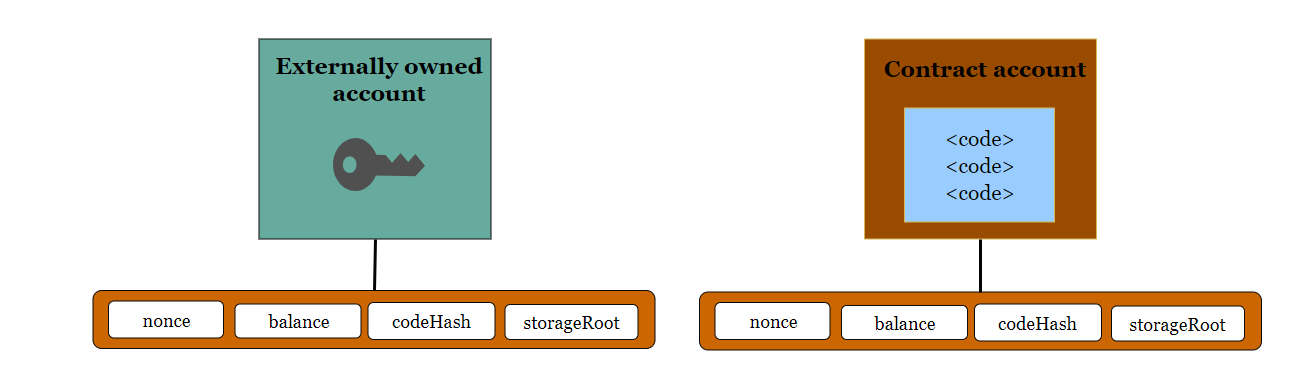
\includegraphics[width=\textwidth]{utentiContratti}
    \caption{Differenza tra utenti esterni e contratti}
\end{figure}

\section{Esecuzione del codice nella blockchain di Ethereum}

Ricordiamo che Solidity è uno dei linguaggi utilizzati per sviluppare Smart Contract sulla piattaforma Ethereum. 
La Ethereum Virtual Machine che esegue lo smart contract non è però in grado di comprendere direttamente il codice scritto in Solidity ed è quindi necessario trasformarlo in un codice di più basso livello.
Il compilatore trasforma il codice scritto in Solidity in un Byte Code.
Quando la virtual machine di Ethereum (EVM) è attiva ha uno stato interno che può essere definito dalla tuple $<blockState, transaction, message, code, memory, stack, pc, gas>$, in blockState abbiamo tutti i dati relativi agli account.
\newline Generalmente l'esecuzione del codice è un loop infinito che scorre tutto il bytecode svolgendo l'operazione indicata dal program counter corrente andandolo poi ad incrementare, si ferma quando viene riscontrato un errore, un return o quando si raggiunge la fine del programma.
Alla fine dell'esecuzione del contratto, è possibile restituire un array di byte.
Lo smart contract ha accesso a tre differenti spazi per il salvataggio dei dati necessari:

\begin{itemize}
\item Stack: una coda LIFO in cui possiamo inserire ed eliminare i valori;
\item Memoria: un array di byte infinito;
\item Memoria a lungo termine: un dizionario [chiave, valore] che rimane per sempre e non si perde dopo l'esecuzione del contratto come i precedenti due.
\end{itemize}

Inoltre può accedere ai seguenti dati:

\begin{itemize}
\item Il valore scambiato;
\item Il mittente con i dati del messaggio che ha inviato
\end{itemize}

E' importante notare che la Virtual Machine di Ethereum è Turing completa, questo vuol dire che con il codice EVM posso svolgere qualsiasi computazione che potrei svolgere con un qualsiasi altro linguaggio, inclusi i loop infiniti.
EVM permette di svolgere i loop in due modi:
\begin{itemize}
\item Abbiamo una istruzione JUMP che mi permette di tornare indietro nel codice andando quindi al punto precedente e una di JUMP condizionale che effettua un controllo (ad esempio la guardia del while con x minore di 100) ed eventualmente effettua un salto;
\item E' inoltre possibile utilizzare la ricorsione andando a chiamare altri contratti
\end{itemize}

Questa seconda possibilità offerta dalla ricorsione presenta però un possibile problema, un utente potrebbe infatti creare un loop infinito di chiamate tra contratti andando quindi a danneggiare anche il miner.
Per risolvere questo possibile problema si è deciso di far impostare un numero massimo di computazioni che possono essere svolte per ogni transazione.
In questo modo il miner che deve eseguire il contratto, svolge la computazione per il numero di passi scelto e poi, una volta terminato il gas segna la transazione come fallita ottenendo comunque il pagamento di una ``tassa`` da chi ha inviato la transazione.
Con gas si intende la quantità massima di moneta digitale scelta dal mittente della transazione che può essere consumata dal miner per l'esecuzione della transazione.


\newpage
\chapter{Complex Graph Analysis}

Nelle sezioni precedenti abbiamo parlato dell'organizzazione di Ethereum e della struttura di blocchi e transazione, conoscere tutte queste informazioni si è rivelato utile per l'ultima parte del tirocinio in cui partendo dal dataset di transazioni siamo riusciti a creare un grafo su cui svolgere l'analisi.
Il grafo prodotto è di grandi dimensioni, abbiamo una quantità di nodi che supera i 6 milioni, ad ogni nodo corrisponde un indirizzo di un account Ethereum, gli archi tra i nodi rappresentano le transazioni che sono state effettuate.

Lo studio dei grafi di grandi dimensioni è una disciplina che ha già ricevuto molta attenzione. Studi di questo genere sono applicati in vari campi come ad esempio l'economia e la biologia con lo scopo di conoscere la conformazione del grafo e l'evoluzione nel tempo.

L'analisi del grafo è stata effettuata utilizzando delle tecniche utilizzate in passato anche con il grafo delle transazioni Bitcoin, come illustrato in \cite{maesa2016uncovering} \cite{maesa2016analysis} \cite{maesa2017data} \cite{maesa2017detecting}, in questa sezione le andiamo a vedere più nel dettaglio.
Gli archi del grafo sono orientati, la nostra analisi ha previsto anche la creazione di una versione del grafo non orientata in cui non vengono differenziate le transazioni ricevute da un nodo da quelle inviate. Oltre allo studio della versione non orientata del grafo, sono state effettuate della analisi anche sulla componente connessa più grande.
\newpage
\section{Analisi dei gradi dei nodi}

L'analisi più semplice riguarda il numero di nodi e di archi che sono presenti all'interno del grafo, in questa fase è anche possibile identificare quali nodi sono isolati.
Risulta particolarmente interessante andare a studiare questi dati anche in relazione al passare del tempo, in modo da visualizzare in un grafico in che modo la rete Ethereum si sia espansa nel corso del tempo. 
Per svolgere un'analisi di questo genere è necessario dividere il dataset in periodi di tempo e lavorare su ognuno di questi grafi.

Un altro dato che può essere estratto abbastanza facilmente analizzando il grafo orientato è la quantità di archi entranti e uscenti da ogni nodo, in particolare è interessante studiare la distribuzione di questi valori e la media.
Lo stesso studio, possiamo svolgerlo anche sul grafo non orientato.
In entrambi i casi è possibile andare a selezionare quei nodi che hanno il maggior numero di archi uscenti (o entranti nel caso del grafo orientato) e questo dato può essere interessante per capire quali sono gli account maggiormente attivi nella rete.

\section{Analisi della centralità dei nodi}

Oltre alla analisi precedenti, è possibile svolgere sul grafo anche delle analisi più complesse, una di queste è la centralità.
Dato un grafo, la centralità è la misura che viene utilizzata per comprendere l'importanza di un nodo, più il nodo è centrale e più è importante per la rete.
La centralità in un grafo sociale viene studiata per capire ad esempio quanto è influente un certo utente in un social network oppure quanto è importante una pagina web. 
Nel caso delle transazioni di Ethereum la utilizziamo per capire quali sono i nodi più importanti per l'economia della rete. 
A causa dell'importanza di questa informazione, sono state sviluppate tante tecniche differenti per calcolare la centralità in un grafo:

\begin{itemize}
    \item \textit{Centralità Armonica} \cite{Harmonic}:  è una misura ``geometrica`` della centralità, questo vuol dire che il calcolo dell'importanza di un nodo dipende dalla sua distanza dagli altri nodi della rete. 
    La formula utilizzata per questa misurazione è la seguente:
    \begin{equation}
    \sum_{v \in V} \frac{1}{d(u,v)}
    \end{equation}
    dove $v$ è un nodo della rete, $V$ è l'insieme di tutti i nodi del grafo mentre la distanza d(u,v) è calcolata come il numero di nodi che si trovano nel cammino più breve tra $u$ e $v$. La centralità in questo caso dipende dal valore della sommatoria, più questo è alto e più il nodo $u$ preso in esame sarà centrale;
 
    \begin{figure}[H]
        \centering
        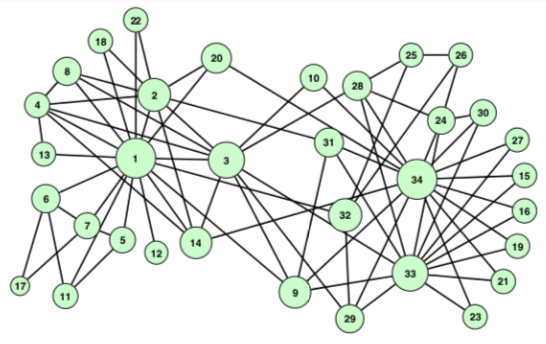
\includegraphics[width=0.6\columnwidth]{Harmonic.png}
        \caption{Centralità armonica del grafo, i nodi più grandi sono i più centrali secondo questa metrica}
    \end{figure}

    \item \textit{Grado}: sulla base di questa misura, i nodi centrali della rete saranno quelli con il maggior numero di archi incidenti, siano essi entranti o uscenti.
    Un esempio di misurazione della centralità tramite il grado dei nodi possiamo vederlo nell'immagine:

    \begin{figure}[H]
        \centering
        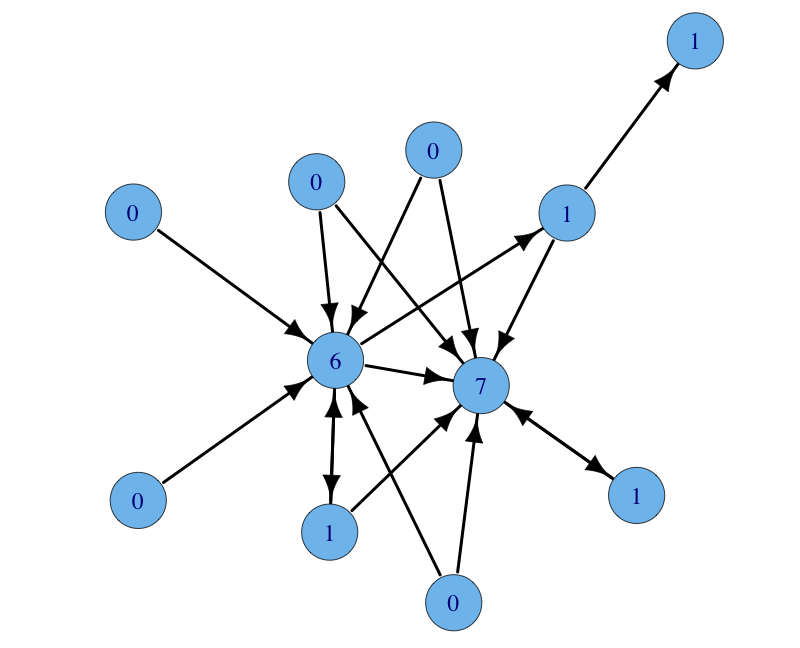
\includegraphics[width=0.5\columnwidth]{indegree.png}
        \caption{I nodi 6 e 7 sono i più centrali per la rete  hanno il maggior numero di nodi incidenti}
    \end{figure}
    \item \textit{Grado entrante}: questa misura di centralità va a calcolare per ogni nodo gli archi entranti, questo ci permette di capire quali sono gli indirizzi che hanno ricevuto maggiori transazioni o, nel caso di un contratto, maggiori chiamate;
    \item \textit{Grado uscente}: in questo caso vale lo stesso discorso della proprietà precedente, calcoliamo però il numero di archi uscenti da ciascun nodo cercando quindi di comprendere quali siano i nodi che effettuano il maggior numero di transazioni.
\end{itemize}
Anche nel caso della centralità è interessante capire come la rete si sia evoluta nel tempo e come siano variati i nodi più importanti temporalmente.
Per il calcolo della centralità sono stati sfruttati gli algoritmi messi a disposizione dal framework WebGraph\cite{WebGraph}.

\section{Analisi delle distanze}

Su un grafo di grandi dimensioni come quello delle transazioni di Ethereum è interessante svolgere anche l'analisi delle distanze. Questa comprende lo studio del diametro, della distanza media dei nodi e la distribuzione di queste distanze.
\newline
La distanza d(u,v) è il numero dei nodi che troviamo lungo il cammino più breve da u a v.
\newline
Con diametro si intende:

\begin{equation}
\max_{(u,v) \in V \times V} d(u,v)
\end{equation}
ovvero la massima lunghezza del cammino minimo tra due nodi presenti all'interno del grafo.
\newline
La distanza media invece è calcolabile con la seguente formula:

\begin{equation}
\frac{1} {|V|^{2}} \sum_{(u,v) \in V \times V} d(u, v) 
\end{equation}
dove per ogni coppia di nodi $(u,v)$ si prende la lunghezza del percorso più breve da $u$ a $v$.
Queste due misurazioni vengono effettuate sul grafo non orientato e sulla componente connessa più grande, per svolgerle è stato utilizzato lo stesso algoritmo sfruttato anche per l'analisi del grafo di Bitcoin \cite{maesa2016uncovering} \cite{maesa2016analysis} \cite{maesa2017data} \cite{maesa2017detecting}.
Questo algoritmo, preso un grafo con n nodi e m archi permette di eseguire il calcolo in $O(m)$.

Una volta calcolato il diametro e le distanze tra le varie coppie di nodi del grafo, è possibile studiare la distribuzione delle distanze.
Questa misurazione indica quante paia di vertici (u,v) si trovano a distanza h.
Dato il grafo $G$ con n nodi, per ogni h con $h > 0$ prendiamo tutte le coppie di nodi (u,v) tali che d(u,v) = h e calcoliamo $N_h$ eseguendo la normalizzazione:

\begin{equation}
N_h = \frac{|\big\{(u,v) \in V\times V \space | \space d(u,v) = h \land u \neq v\big\}|} {n(n-1)}
\end{equation}


\chapter{Strumenti utilizzati}

Durante il tirocinio abbiamo utilizzato molti strumenti open source disponibili su GitHub, li descriviamo brevemente in questo capitolo cercando di concentrarci in particolar modo sulle funzioni che sono state più utili per i nostri scopi.

\section{Geth}

Durante il tirocinio abbiamo sfruttato moltissimo Go Ethereum, si tratta dell'implementazione in Go \cite{GoLang} del protocollo Ethereum, questo progetto è totalmente open source ed è disponibile su GitHub \cite{goEthereum}.
Go Ethereum mette a disposizione delle librerie utilizzabili in progetti Android e iOS e soprattutto il client Geth che abbiamo sfruttato per vari scopi.

Abbiamo usato Geth da terminale principalmente per due scopi, la sincronizzazione della blockchain di Ethereum e l'estrazione delle transazioni.
Per quanto riguarda la sincronizzazione, Geth ha consentito di utilizzare i nostri computer come nodi della rete Ethereum e quindi di scaricare in locale le informazioni presenti nella blockchain.
La sincronizzazione è stata svolta in modalità ``full``, sono stati scaricati tutti i blocchi, dal primo all'ultimo comprese le transazioni contenute all'interno.
Abbiamo svolto l'operazione di sincronizzazione su un computer munito di disco SSD, questo ha permesso una maggiore velocità rispetto al disco meccanico che abbiamo provato ad utilizzare originariamente. Nel complesso sono stati necessari circa 20 giorni per avere in locale tutta la blockchain di Ethereum.

In alternativa sarebbe anche stato possibile configurare Geth come ``Light Node``, in questo modo avremmo limitato la quantità dei dati scaricati perché sarebbero stati recuperati solamente gli header di tutti i blocchi, ma non le transazioni. Questa seconda opzione però non faceva al caso nostro perchè non avremmo avuto accesso ai dati delle transazioni, quindi l'abbiamo subito scartata.
\newline Geth per il salvataggio delle transazioni sfrutta LevelDB, una libreria scritta in Go da Google e disponibile su Github \cite{LevelDB} che permette di salvare coppie (chiave, valore) in un database.

Per massimizzare la velocità e per utilizzare anche strumenti aggiuntivi, abbiamo avviato Geth con varie opzioni:
\begin{itemize}
\item -rpc --rpcport 8545 --rpcaddr 127.0.0.1 --rpccorsdomain ``*``: Avendo la necessità di sincronizzare la blockchain e contemporaneamente estrarre i dati contenuti al suo interno, abbiamo dovuto avviare Geth con questi flag. 
In particolare il flag -rpc ci permette di attivare il protocollo JSON-RPC (JSON-Remote Procedure Call) \cite{JSONRPC}, questo consente di inviare a Geth delle richieste tramite HTTP o tramite Socket e poi ricevere le risposte. Gli altri flag servono semplicemente per scegliere l'indirizzo da utilizzare per le richieste e la corrispondente porta.
Questo ci ha permesso di sincronizzare la blockchain e nel frattempo inviare a Geth richieste riguardanti i blocchi già salvati in locale.
\item --cache=4096: Valore massimo di memoria RAM in Megabytes che Geth avrebbe potuto allocare. Questa opzione è stata utile per velocizzare la sincronizzazione;
\item --web3: Opzione che abbiamo usato per permettere l'utilizzo degli strumenti messi a disposizione dalla libreria Web3JS per estrarre le informazioni dai blocchi e dalle transazioni presenti nella blockchain;
\item --debug: Questa opzione è stata decisamente utile per comprendere lo status delle transazioni nei blocchi precedenti all'Hard Fork Byzantium \cite{Byzantium}. Sfortunatamente ha anche comportato una maggiore quantità di tempo necessaria per sincronizzare la blockchain e per estrarre le informazioni da essa.
\end{itemize}

Geth è stato utilizzato anche per la fase di estrazione dei dati dalla blockchain, questo tool infatti mette a disposizione anche una console Javascript, questa può essere avviata sempre da terminale tramite il comando ``console``, al momento dell'avvio è necessario collegarla ad un nodo della rete Ethereum.
La console permette un utilizzo interattivo in cui si può semplicemente scrivere dei comandi e ricevere delle risposte (ad esempio i dettagli di un blocco o di una transazione) e un uso non interattivo in cui si avvia chiedendo l'esecuzione di uno script salvato in locale sulla nostra macchina.
Per l'estrazione dei dati delle transazioni abbiamo utilizzato la versione non interattiva della console che ci ha consentito di eseguire uno script e di salvare l'output su file.


\section{WebGraph}

WebGraph \cite{WebGraph} è un framework sviluppato da Paolo Boldi e Sebastiano Vigna dell'università di Milano.
Si tratta di un framework per la compressione di grafi che permette di gestire efficientemente grandi quantità di dati sfruttando le tecniche di compressione più moderne.
WebGraph ci fornisce sia dei metodi di compressione che permettono di ridurre le dimensioni dei grafi sia dei metodi che consentono di navigare all'interno del grafo già compresso senza doverlo decomprimere.
Abbiamo utilizzato WebGraph per creare il grafo delle transazioni della rete Ethereum partendo dai dati estratti dalla Blockchain.
Successivamente sempre tramite WebGraph abbiamo svolto l'analisi del grafo sfruttando gli strumenti di analisi messi a disposizione.


\section{Librerie Utilizzate}

Durante il tirocinio sono state utilizzate diverse librerie esterne trovate principalmente su GithHub:

\begin{itemize}
    \item Nella primissima parte del tirocinio abbiamo utilizzato la libreria EthereumJ \cite{EthereumJ}, una implementazione in Java del protocollo Ethereum. In particolare sono stati sfruttati i moduli riguardanti la decodifica di stringhe codificate con RLP, il formato di encoding usato da Ethereum che verrà analizzato in dettaglio nel capitolo 4.
    \item Un altro strumento che ci è stato particolarmente utile è Web3JS, si tratta di una libreria open source e disponibile su GitHub \cite{Web3JS} che ci ha consentito di estrarre tutti i dati delle transazioni dalla blockchain Ethereum.\newline
    Per il tirocinio abbiamo utilizzato in particolare 3 funzioni messe a disposizione da Web3JS:
        \begin{itemize}
            \item getBlock(blockNum): questa funzione prende in input il numero di un blocco presente nella blockchain e ci restituisce in formato JSON tutti i campi contenuti al suo interno. Tra i vari campi è particolarmente interessante la lista degli hash delle transazioni contenute all'interno del blocco, questa informazione verrà utilizzata dalla funzione getTransaction;
            \item getTransaction(hash): questa funzione prende in input l'hash di una transazione e restituisce tutti i dettagli relativi in formato JSON;
            \item getTransactionReceipt(hash): questa funzione prende in input l'hash di una transazione e restituisce i dettagli del receipt della transazione in formato JSON. Abbiamo utilizzato questa funzione per recuperare il mittente di ogni singola transazione.
            \begin{figure}[H]
                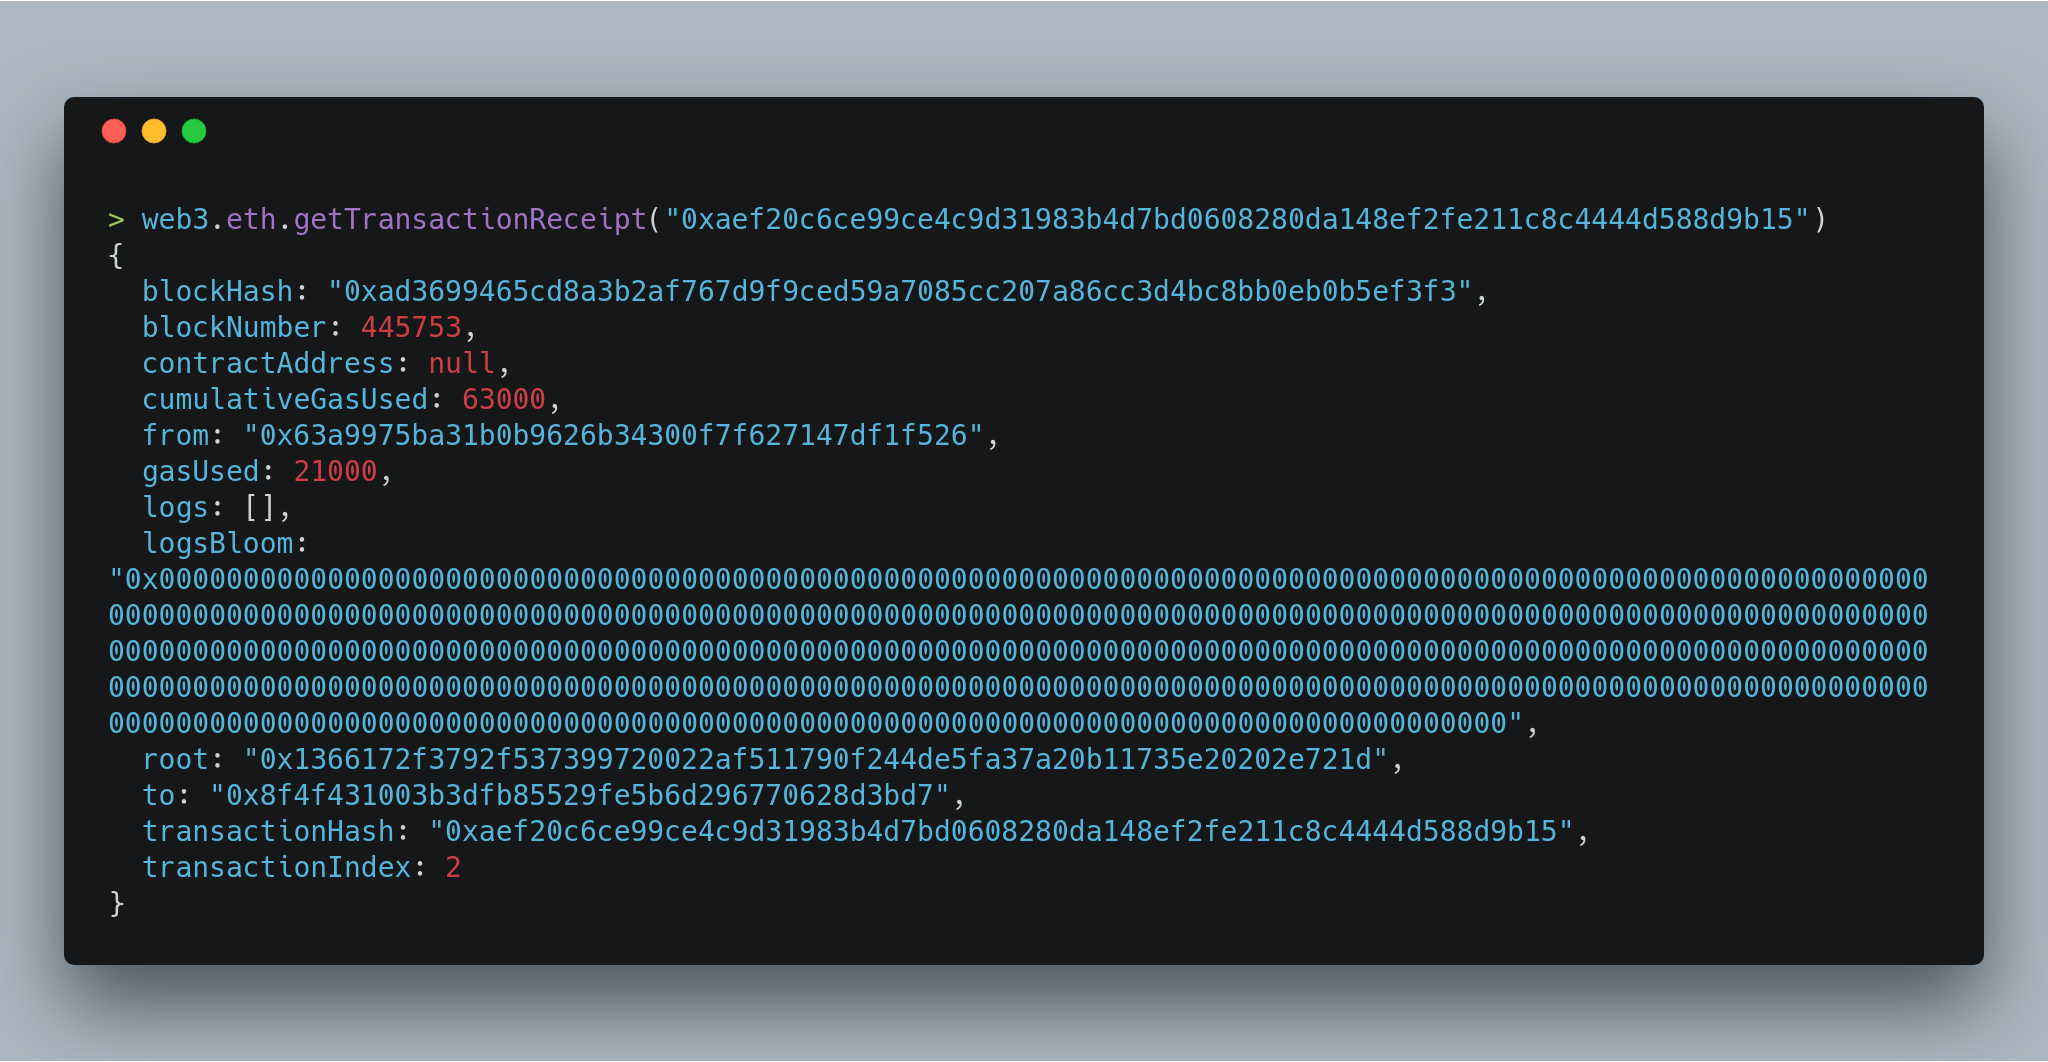
\includegraphics[width=\textwidth]{carbon-10}
                \caption{Esempio di richiesta di un transaction receipt}
            \end{figure}
        \end{itemize}
    \item Per svolgere alcuni test sulla decodifica di stringhe codificate con RLP ci è stata utile la libreria ``RLP Javascript`` \cite{RLPGitHub} che ci ha permesso tramite il terminale di capire in che modo venissero suddivise le stringhe.
    \item Per la generazione dei grafici che rappresentano i risultati dell'analisi dei dati estratti dalla blockchain abbiamo utilizzato due librerie scritte in Python, si tratta di Seaborn\cite{Seaborn} e di MatPlotLib\cite{MatPlotLib}.
\end{itemize}


\chapter{Analisi del grafo}

In questo capitolo viene descritto tutto il lavoro svolto durante il tirocinio. Inizialmente verranno esposti i dettagli riguardanti RLP, l'encoding utilizzato da Ethereum successivamente andremo a descrivere la struttura interna di un blocco, di una transazione e di una receipt.
Verranno inoltre descritti i due possibili metodi che possono essere utilizzati per il parsing della blockchain di Ethereum mettendone in evidenza i pro e i contro.

\section{Encoding dei dati della blockchain}

Come già illustrato in precedenza, l'obiettivo del tirocinio è stato quello di parsare i dati della blockchain di Ethereum rendendone leggibile il contenuto.
È essenziale quindi capire come Ethereum codifichi tutte le informazioni contenute nelle transazioni.
Leggendo la Wiki di Ethereum \cite{RLP} abbiamo  analizzato RLP (Recursive Length Prefix) ovvero la codifica utilizzata per serializzare blocchi e transazioni trasformandoli in array di byte.

L'encoding di dati viene effettuato seguendo alcune regole basilari:

\begin{itemize}
\item Se si deve codificare 1 singolo byte e il suo valore è compreso tra 0 e 127 (0x00 e 0x7f se siamo in hex) allora si scrive direttamente lo stesso identico byte anche nel formato RLP senza aggiungere o modificare altro.
Per verificare l'affermazione precedente, la Figura 2.3 mostra come viene utilizzata la libreria RLP scritta in Javascript e disponibile su GitHub \cite{RLPGitHub};

\begin{figure}[H]
    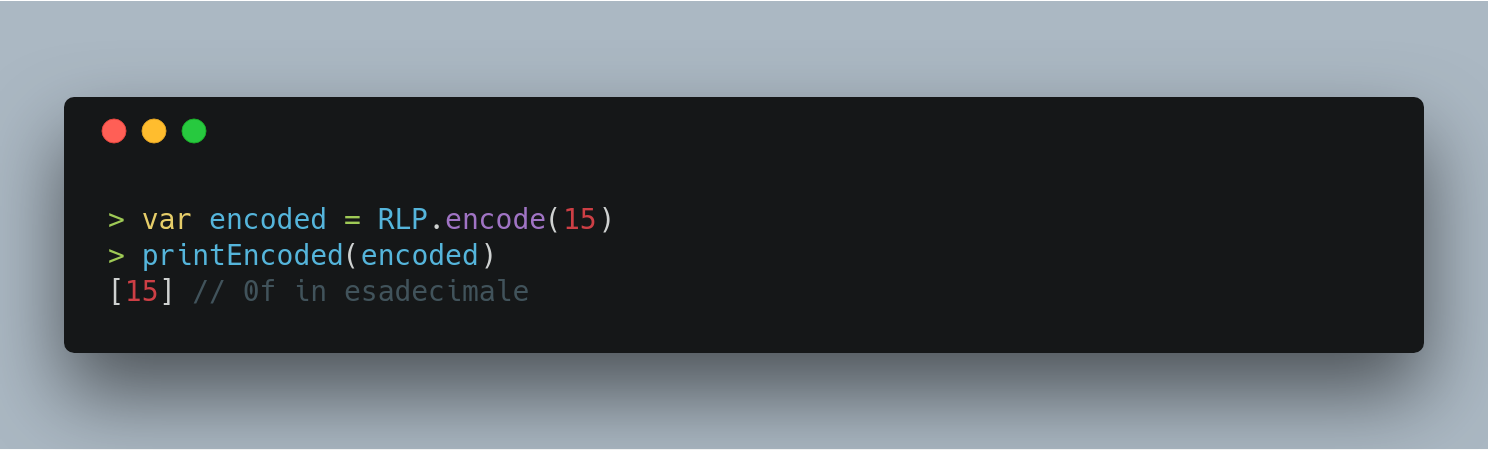
\includegraphics[width=\textwidth]{carbon-2} 
    \caption{Codifica di un singolo byte}
\end{figure}

\item Se abbiamo una stringa con lunghezza compresa tra 2 e 55 byte, la codifica RLP prevede un singolo byte iniziale in cui indichiamo la lunghezza della stringa sommato a 128 (0x80) seguito poi dai bytes originali che vogliamo codificare.

\begin{figure}[H]
    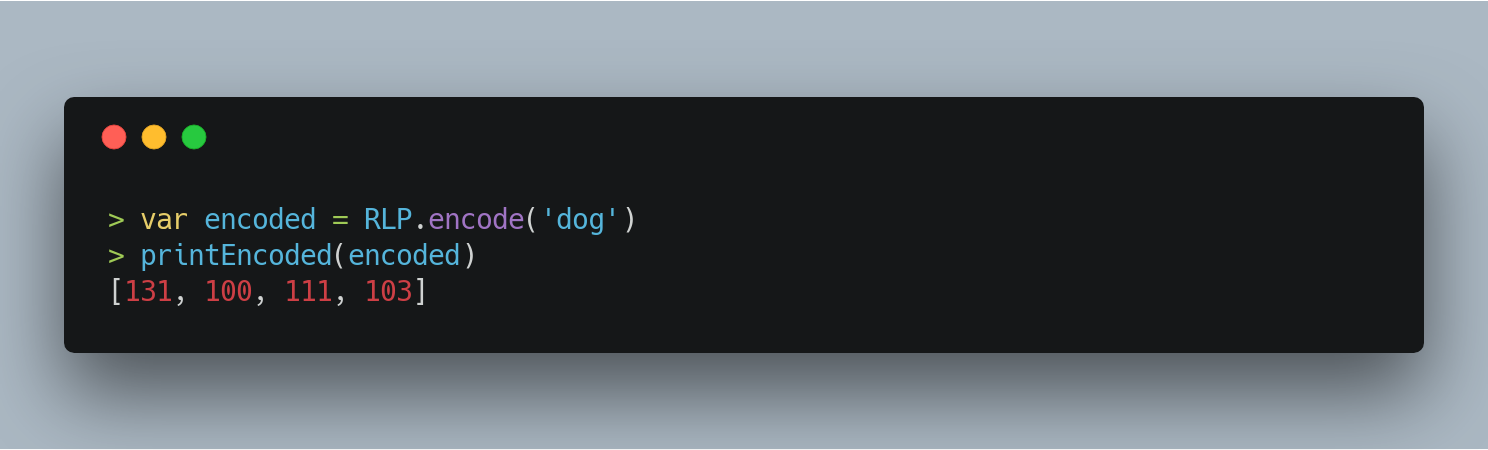
\includegraphics[width=\textwidth]{carbon-3}
    \caption{Codifica di una stringa con lunghezza compresa tra 2 e 55 bytes}
\end{figure}

Come possiamo vedere anche dallo screenshot mostrato nella Figura 2.4, la parola dog viene codificata con un array di byte, in particolare il primo ha valore 131 ovvero 128 + 3, dove quest'ultima cifra rappresenta la lunghezza della stringa;

\item Se la stringa supera i 55 bytes allora la codifica è composta da 3 parti. 
La prima parte è un singolo byte con valore 183 più la lunghezza in byte della seconda parte. 
La seconda parte è il valore in hex della lunghezza della stringa. L'ultima parte è la stringa codificata.
Ad esempio per la stringa ``Lorem ipsum dolor sit amet, consectetur adipisicing elit`` abbiamo una lunghezza di 56 bytes e il primo byte della stringa codificata sarà quindi 183 + 1 (1 bytes per il valore 56);
\begin{figure}[H]
    \centering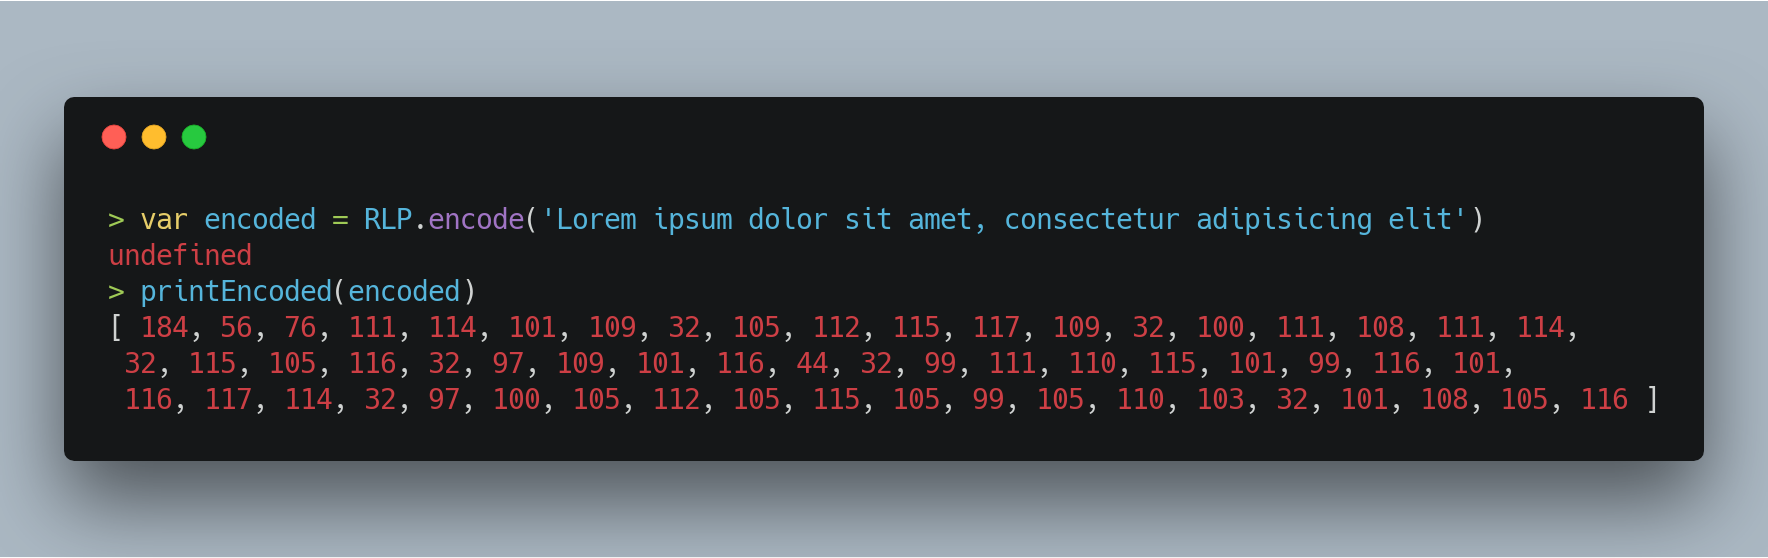
\includegraphics[width=\textwidth]{carbon-4}
    \caption{Codifica di una stringa con lunghezza maggiore di 55 byte}
\end{figure}


\item Se codifichiamo un array e la lunghezza è compresa tra 0 e 55 bytes, la codifica consiste in un array di byte in cui il primo elemento rappresenta la lunghezza dell'array + 192 seguito dalla codifica RLP dei vari elementi dell'array basandoci sulle regole precedenti;

\begin{figure}[H]
    \centering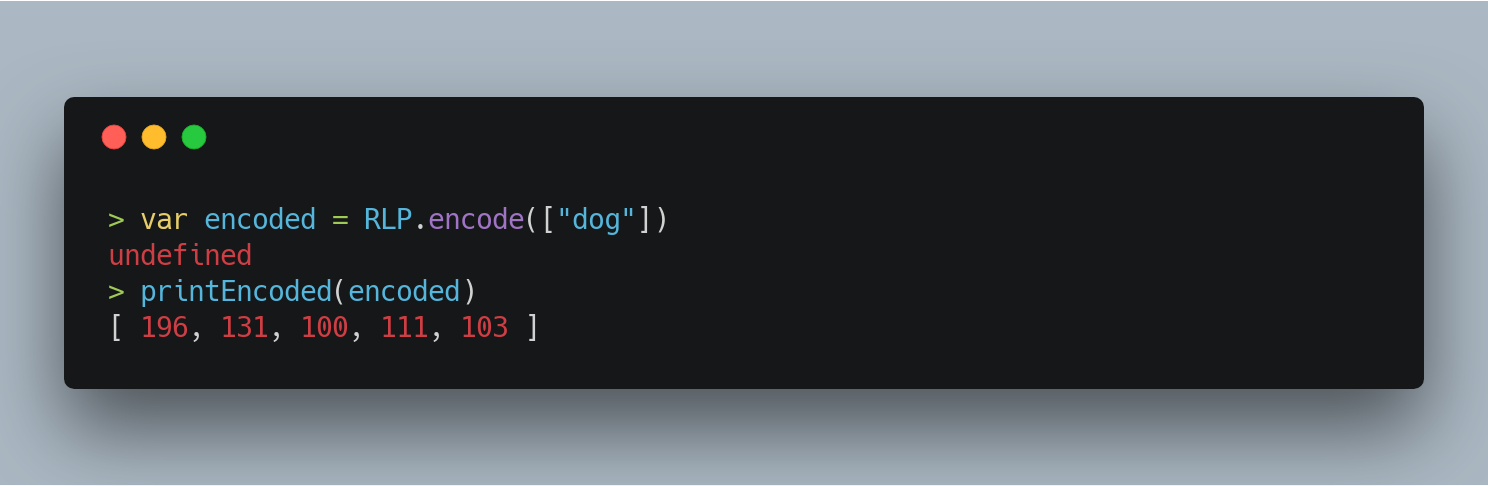
\includegraphics[width=\textwidth]{carbon-5}
    \caption{Codifica di un array con lunghezza compresa tra 0 e 55 byte}
\end{figure}


\item Se codifichiamo un array la cui lunghezza supera i 55 bytes allora la codifica consiste in 3 parti.
La prima è un singolo byte con valore 247 più la lunghezza in byte della seconda.
La seconda è la lunghezza totale di tutti gli elementi dell'array.
L'ultima è la concatenazione della codifica dei vari valori contenuti nell'array, codificati con i metodi indicati sopra.



\end{itemize}
\newpage
\section{Struttura di un blocco della blockchain di Ethereum}

Dopo aver capito il funzionamento di RLP e aver individuato una libreria su GitHub che gestisse la decodifica di stringhe RLP siamo passati ad analizzare il contenuto di un blocco della blockchain di Ethereum studiando lo ``Yellow Paper`` \cite{YellowPaper}.
Il contenuto del blocco è codificato tramite il formato RLP seguendo le regole elencate in precedenza, in particolare i primi byte della stringa del blocco indicano la lunghezza complessiva del blocco.
Conoscere la lunghezza complessiva del blocco è stato utile nella prima fase del parsing per analizzare un file di testo con tutti i blocchi codificati e separare i vari blocchi per poi analizzarne il contenuto.

Ogni blocco presente nella blockchain di Ethereum è composto da un header con varie informazioni e dalla lista delle transazioni che si trovano al suo interno.

\begin{figure}[H]
    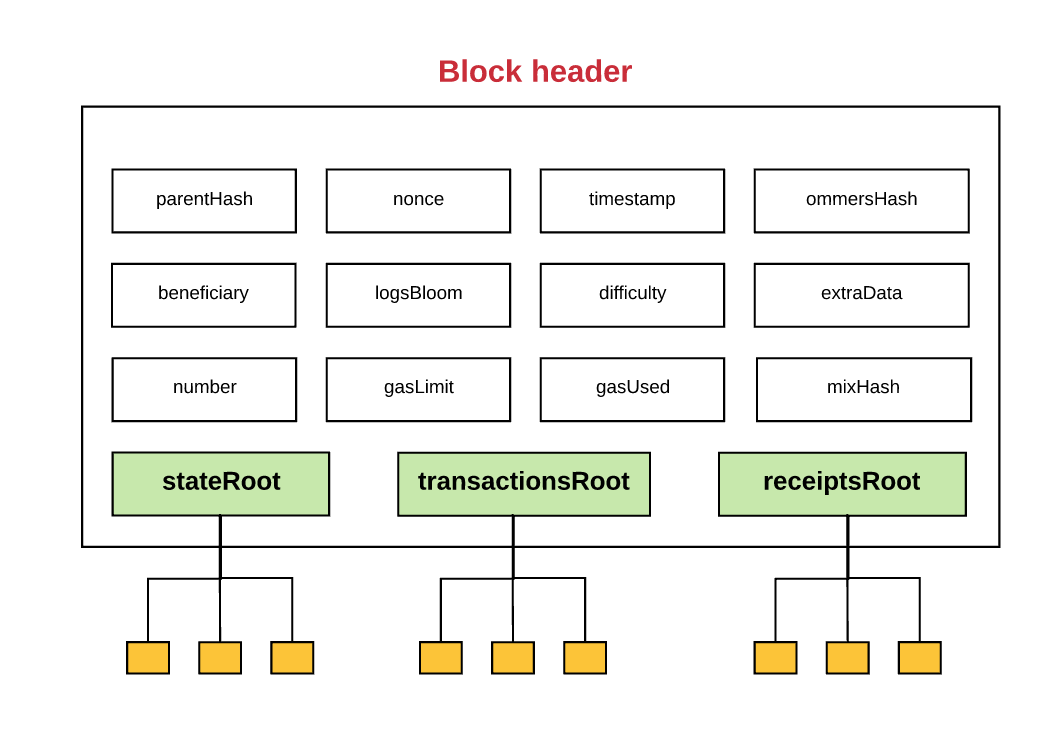
\includegraphics[width=\textwidth]{BlockHeader}
    \caption{Struttura di un blocco}
\end{figure}


\begin{itemize}
\item \textit{parentHash}: hash di 256 bit che rappresenta l'hash del precedente blocco contenuto all'interno della blockchain;
\item \textit{nonce}: una stringa di 64 bit che viene utilizzata con il mixHash per dimostrare che il miner ha svolto una computazione sufficiente per generare il blocco;
\item \textit{timestamp}: valore che indica quando il blocco è stato inserito all'interno della blockchain;
\item \textit{ommersHash}: hash di 256 bit che rappresenta la lista dei blocchi che hanno il parentHash uguale al parentHash del blocco precedente nella blockchain;
\item \textit{beneficiary}: Indirizzo di 160 bit che rappresenta l'utente che ha svolto il mining del blocco e che quindi otterrà il compenso stabilito da Ethereum;
\item \textit{logsBloom}: campo da 2048 bit si tratta del riferimento ad una struttura dati denominata Bloom filter. 
Questa struttura dati viene utilizzata per ridurre al minimo la memorizzazione di dati duplicati, quando una transazione viene verificata, i log vengono inseriti nel bloom filter ma non tra i dati del blocco in modo da risparmiare spazio.
Se volessimo andare a controllare i log di una certa transazione ci basterà scorrere il logsBloom che è rappresentato come un array di byte, nel caso in cui dovessimo trovare qualcosa di utile andremo poi a prendere la singola transazione che ci interessa e la eseguiremo generando i log; \cite {BloomFilter}
\item \textit{difficulty}: il valore numerico che rappresenta il livello di difficoltà per il mining del blocco. Il valore può essere calcolato prendendo timestamp e difficulty del blocco precedente;
\item \textit{extraData}: Campo lungo al più 32 bytes che può contenere informazioni utili per questo blocco;
\item \textit{gasLimit}: valore numerico che indica il massimo gas che può essere speso per il blocco;
\item \textit{gasUsed}: il valore numerico che indica il gas speso dalle transazioni che troviamo nel blocco;
\item \textit{mixHash}: hash di 256 bit che, combinato con il nonce, dimostra che il miner ha svolto una computazione sufficiente per generare il blocco;
\item \textit{stateRoot}: l'hash di 256 bit del root node del ``world state`` in cui troviamo tutte le informazioni riguardanti gli account della blockchain. Questa struttura dati viene aggiornata dopo aver eseguito e confermato tutte le transazioni del blocco;
\item \textit{transactionsRoot}: l'hash di 256 bit del nodo root della struttura ad albero in cui vengono inserite tutte le transazioni presenti all'interno del blocco;
\item \textit{receiptsRoot}: l'hash di 256 bit del nodo root della struttura ad albero in cui troviamo i receipt ovvero un log di tutte le transazioni presenti all'interno del blocco. Per il tirocinio abbiamo sfruttato i receipt per recuperare lo status di una transazione (fallita/eseguita).
\end{itemize}

Riportiamo come esempio il contenuto dell'header del blocco 1613030 ottenuto tramite Etherscan\cite{Etherscan} e codificato secondo la codifica RLP:
\begin{figure}[H]
    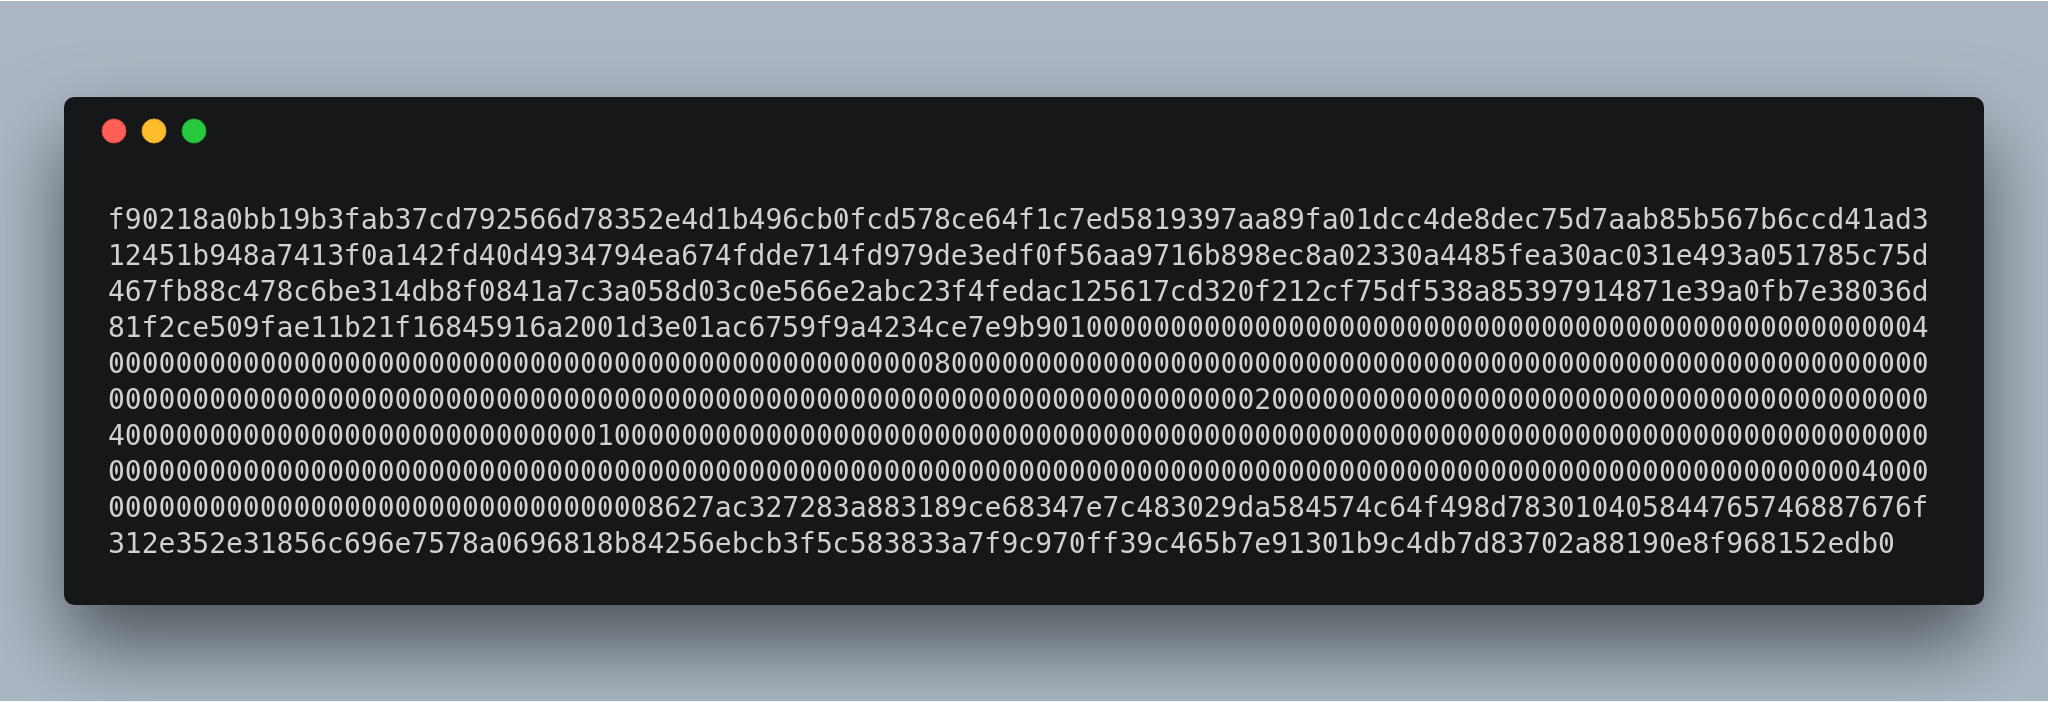
\includegraphics[width=\textwidth]{carbon-7}
    \caption{Stringa esadecimale che rappresenta l'header di un blocco}
\end{figure}
\newpage
Analisi del blocco:
\newline
\textit{f9} = dimensione del campo che indica la lunghezza del blocco in byte.
249 in questo caso a cui va sottratto 247 per ottenere 2 che è la lunghezza del campo successivo;

\textit{0218} = lunghezza complessiva del blocco in byte (536);

\textit{a0} = lunghezza del campo parentHash (a0 equivale a 160, togliendo 128 abbiamo 32 byte di lunghezza del prossimo campo);

\textit{bb19b3fab37cd792566d78352e4d1b496cb0fcd578ce64f1c7ed5819397aa89f} = campo parentHash del blocco, la lunghezza è 32 byte;

\textit{a0} = lunghezza del campo ommersHash (a0 equivale a 160, togliendo 128 abbiamo 32 byte di lunghezza del prossimo campo);

\textit{1dcc4de8dec75d7aab85b567b6ccd41ad312451b948a7413f0a142fd40d49347} = campo ommersHash del blocco;

\textit{94} lunghezza dell'indirizzo del miner (94 equivale a 148, togliendo 128 abbiamo 20 byte di lunghezza del prossimo campo ovvero i 160 bit dell'indirizzo);

\textit{ea674fdde714fd979de3edf0f56aa9716b898ec8}: indirizzo dell'utente che ha svolto il mining del blocco;

\textit{a0} = lunghezza del campo stateRoot (a0 equivale a 160, togliendo 128 abbiamo 32 byte di lunghezza del prossimo campo);

\textit{2330a4485fea30ac031e493a051785c75d467fb88c478c6be314db8f0841a7c3}: campo stateRoot;

\textit{a0} = lunghezza del campo transactionsRoot (a0 equivale a 160, togliendo 128 abbiamo 32 byte di lunghezza del prossimo campo);

\textit{58d03c0e566e2abc23f4fedac125617cd320f212cf75df538a85397914871e39}: hash del nodo root dell'insieme delle transazioni del blocco;

\textit{a0} = lunghezza del campo receiptsRoot (a0 equivale a 160, togliendo 128 abbiamo 32 byte di lunghezza del prossimo campo);

\textit{fb7e38036d81f2ce509fae11b21f16845916a2001d3e01ac6759f9a4234ce7e9} = hash del nodo root dell'insieme dei receipt delle transazioni del blocco;

\textit{b901} = lunghezza del campo logsBloom;

\textit{0000000000000000000000000000000000000000000000000400000000000000000000
\newline
000000000000000000000000000008000000000000000000000000000000000000000000000000
000000000000000000000000000000000000000000000000000000000000000000000000000000
200000000000000000000000000000000000000040000000000000000000000000000100000000
000000000000000000000000000000000000000000000000000000000000000000000000000000
000000000000000000000000000000000000000000000000000000000000000000000000000000
000000000000000000400000000000000000000000000000000000}: campo logsBloom del blocco;

\textit{86} = lunghezza del campo difficulty (86 equivale a 134, togliendo 128 abbiamo 6 byte di lunghezza del prossimo campo);
\textit{27ac327283a8} = campo difficulty del blocco;

\textit{83} = lunghezza del campo number (86 equivale a 131, togliendo 128 abbiamo 3 byte di lunghezza del prossimo campo);
\textit{189ce6} = campo number del blocco;

\textit{83} = lunghezza del campo gasLimit (83 equivale a 131, togliendo 128 abbiamo 3 byte di lunghezza del prossimo campo);
\textit{47e7c4} = campo gasLimit del blocco;

\textit{83} = lunghezza del campo gasUsed (83 equivale a 131, togliendo 128 abbiamo 3 byte di lunghezza del prossimo campo);
\textit{029da5} = campo gasUsed del blocco;

\textit{84} = lunghezza del campo timestamp (84 equivale a 132, togliendo 128 abbiamo 4 byte di lunghezza del prossimo campo);
\textit{574c64f4} = campo timestamp del blocco;

\textit{98} = lunghezza del campo extraData (98 equivale a 152, togliendo 128 abbiamo 24 byte di lunghezza del prossimo campo);\newline
\textit{d783010405844765746887676f312e352e31856c696e7578} = campo extraData del blocco;

\textit{a0} = lunghezza del campo mixHash (a0 equivale a 160, togliendo 128 abbiamo 32 byte di lunghezza del prossimo campo);

\textit{696818b84256ebcb3f5c583833a7f9c970ff39c465b7e91301b9c4db7d83702a} = campo mixHash del blocco;

\textit{88} = lunghezza del campo nonce (88 equivale a 136, togliendo 128 abbiamo 8 byte di lunghezza del prossimo campo);

\textit{190e8f968152edb0} = campo nonce del blocco.

\newpage
\section{Struttura e validazione di una transazione}

Dopo aver analizzato il contenuto di un blocco presente all'interno della blockchain è stata studiata la struttura delle transazioni basata sulla definizione che si può trovare nello Yellow Paper \cite{YellowPaper}.
Ethereum prevede i seguenti tipi di transazioni:

\begin{itemize}
    \item Da utente esterno ad utente esterno;
    \item Da utente esterno a contratto;
    \item Da utente esterno ad un indirizzo composto da soli 0, le transazioni di questo tipo sono utilizzate per richiedere la creazione di un nuovo smart contract. Nell'analisi svolta abbiamo considerato l'indirizzo del contratto creato come destinatario della transazione;
    \item Da contratto ad altro contratto, questa tipologia di transazione non è stata considerata durante il nostro studio dei dati della blockchain a causa del troppo tempo necessario per eseguire il codice del contratto destinatario del messaggio.
\end{itemize}

Tutti i tipi di transazione hanno al loro interno le seguenti infomazioni:

\begin{itemize}
\item \textit{Nonce}: valore numerico che rappresenta il numero di transazioni inviate dal mittente, ad ogni nuova transazione viene incrementato. Il nonce viene anche utilizzato per la protezione dai replay attack;
\item \textit{gasPrice}: valore numerico che rappresenta il numero di Wei da pagare per ogni unità di gas che viene consumato durante l'esecuzione della transazione;
\item \textit{gasLimit}: il valore numerico che rappresenta la massima quantità di gas che può essere consumata svolgendo questa transazione;
\item \textit{to}: il destinatario del messaggio, se è un utente esterno abbiamo una indirizzo di 160bit, nel caso della creazione di contratto abbiamo 0;
\item \textit{value}: il numero di Wei che devono essere trasferiti verso l'utente esterno oppure al contratto che stiamo creando;
\item \textit{v, r, s}: valori che rappresentano la firma della transazione, servono per calcolare il mittente.
\end{itemize}

Nelle sole transazioni tra utenti e verso contratti è previsto un altro campo che è ``data`` e può essere utilizzato per inserire un array di byte di lunghezza illimitata, questo viene sfruttato per specificare l'input del contratto quando avviene la chiamata.
Esclusivamente nelle transazioni per la creazione di un contratto Ethereum mette a disposizione un ulteriore campo che serve per inserire il codice che verrà eseguito ad ogni successiva chiamata.

L'utente che vuole inviare sulla rete Ethereum una transazione deve avere a disposizione una coppia chiave privata, chiave pubblica.
Una transazione (da utente a utente o da utente a contratto) può essere costruita nel modo seguente, tra i vari campi non viene specificato il mittente perché verrà generato partendo dalla firma che apporrà l'utente. Nei seguenti esempi viene mostrato come si possono generare diversi campi della transazione mediante l'utilizzo della libreria Web3JS. \cite{Web3JS}.

\begin{figure}[H]
    \centering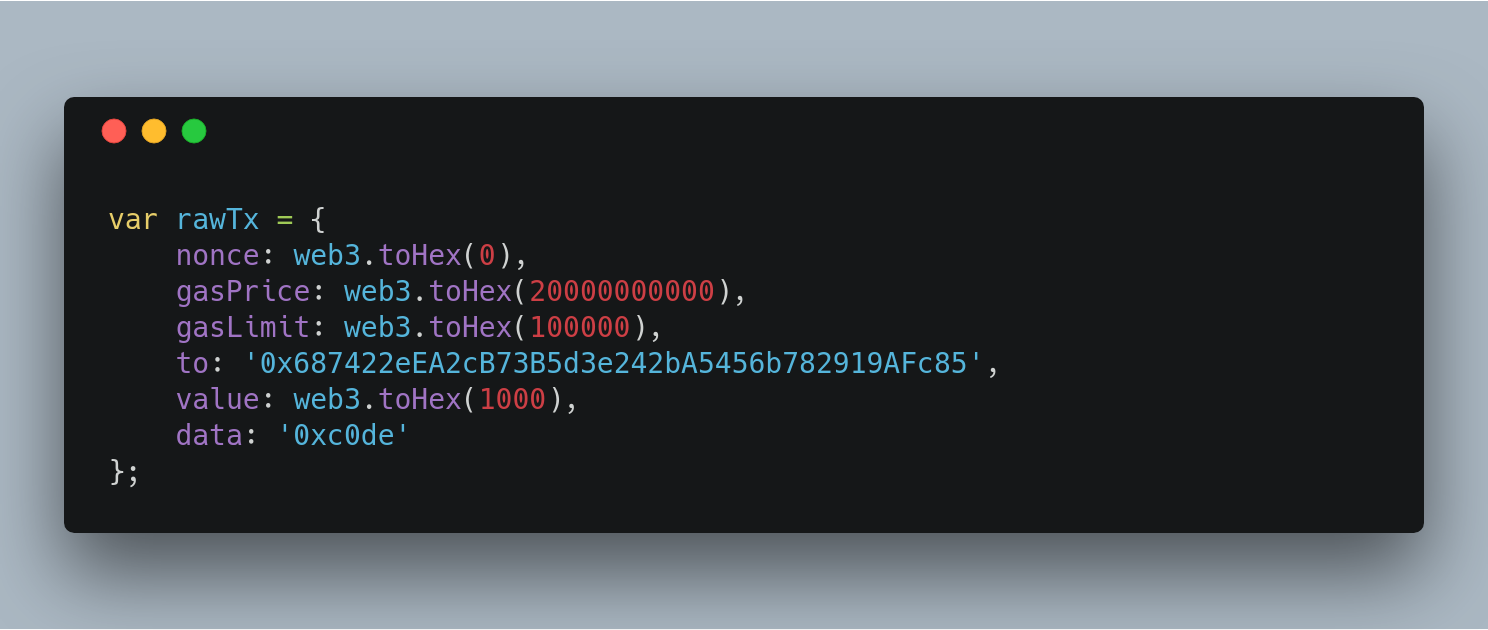
\includegraphics[width=0.8\textwidth]{carbon-8}
    \caption{Creazione di una transazione}
\end{figure}


Dopo aver creato la struttura che contiene tutte le informazioni necessarie alla transazione, l'utente deve utilizzare la sua chiave privata per firmarla. Questo passaggio è essenziale per provare alla rete che chi sta inviando la transazione è effettivamente il proprietario dell'account mittente.

\begin{figure}[H]
    \centering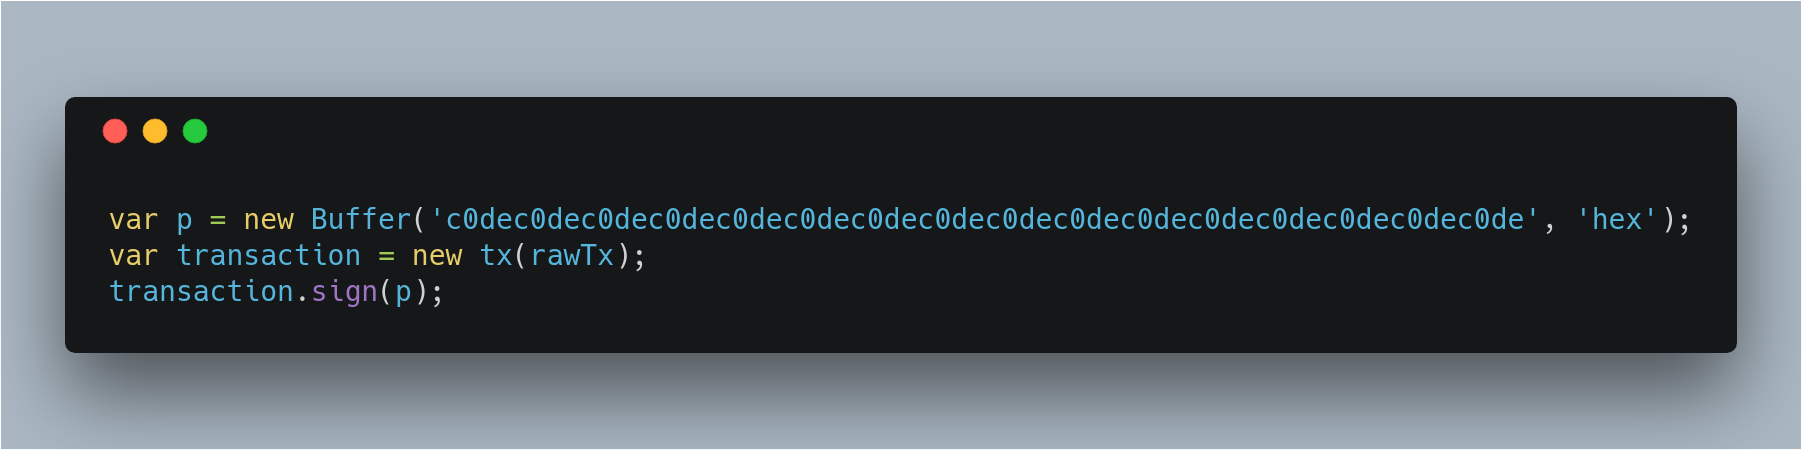
\includegraphics[width=\textwidth]{carbon-9}
    \caption{Firma della transazione}
\end{figure}

\newline
Una volta che alla struttura iniziale vengono aggiunti i campi v, r, s descritti in precedenza, è possibile codificarla con RLP. La stringa risultante viene data in pasto all'algoritmo di hashing Keccak-256 in modo da produrre un hash di 256 bit.

\begin{figure}[H]
    \centering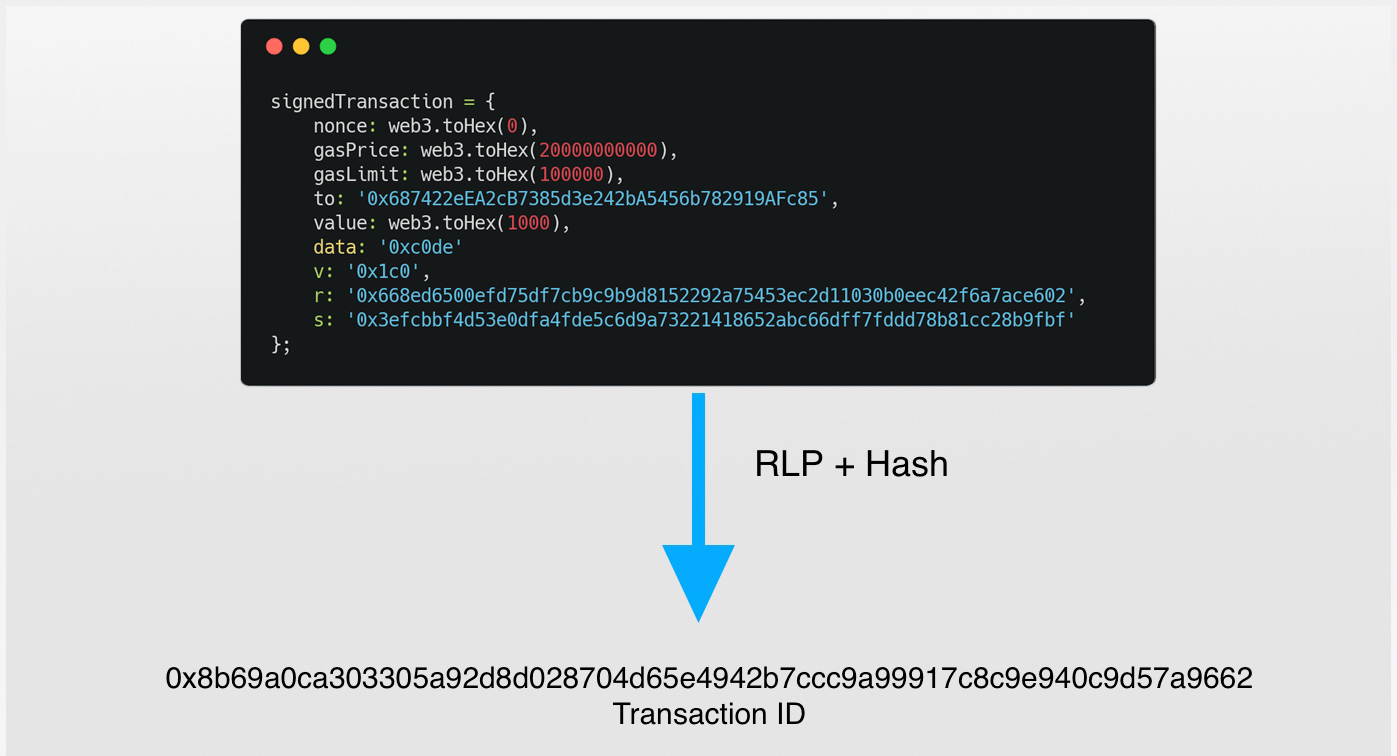
\includegraphics[width=\textwidth]{rlpHash}
    \caption{Hash della transazione}
\end{figure}

Arrivati a questo punto la transazione viene prima validata dal nodo Ethereum locale che controlla che la firma sia corretta, successivamente viene inviata in broadcast ai peer della rete, questi a loro volta invieranno la transazione in broadcast ad altri peer.
Una volta che la transazione è stata inviata sulla rete, viene restituito un id univoco che l'utente può utilizzare per visualizzarne lo status.

\begin{figure}[H]
    \centering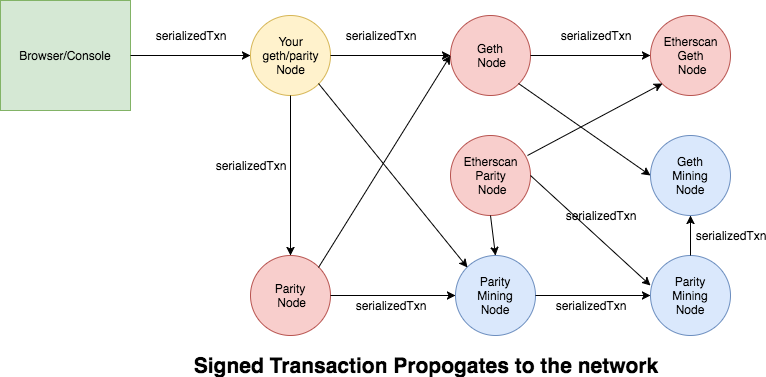
\includegraphics[width=0.7\textwidth]{broadcast}
    \caption{Propagazione di una transazione nella rete}
\end{figure}


La transazione che viene inviata in broadcast non è ancora in un blocco all'interno della blockchain, per questo ultimo ma indispensabile passaggio è necessario il lavoro dei miner.
I miner quando ricevono la transazione inviata in broadcast la salvano in una struttura dati ordinandola in base al campo ``gasPrice``, più questo è alto più è probabile che la transazione venga inserita nella blockchain nel minor tempo possibile.
Una volta che i miners hanno deciso le transazioni da includere in un blocco, queste devono essere validate tramite il processo detto mining e inizia la fase di ``Proof of Work``. Quando uno dei miner risolve il ``puzzle`` e produce quindi un blocco valido, può aggiungerlo alla blockchain. 
All'interno del blocco appena aggiunto troveremo anche la nostra transazione.
\begin{figure}[H]
    \centering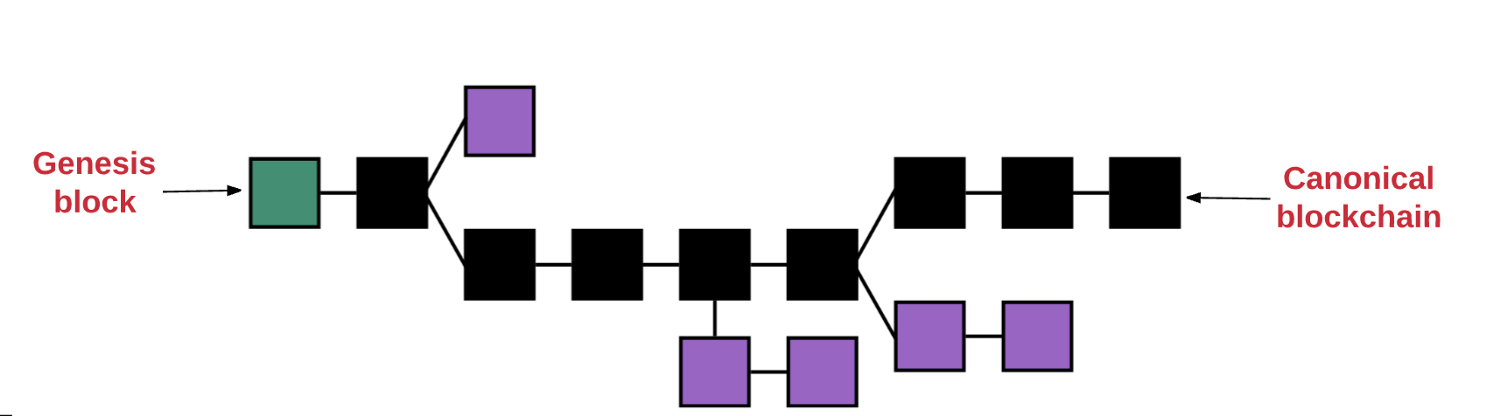
\includegraphics[width=0.8\textwidth]{Fork}
    \caption{Fork della blockchain}
\end{figure}

Se i miner non dovessero essere tutti d'accordo sulla validazione di un blocco, potrebbe capitare che nella blockchain finisca un blocco che non tutti hanno accettato. In questo caso ci troveremmo davanti ad un fork della blockchain che andrebbe a danneggiare l'intero sistema.
Ethereum per evitare questa situazione adotta un protocollo chiamato GHOST, che indica ai miner quale path della blockchain utilizzare basandosi sulla computazione svolta al suo interno. Più è elevato lo sforzo computazionale necessario per arrivare alla foglia e più possibilità ci sono di scegliere quel path.


\section{Struttura di una Transaction Receipt}

Ad ogni transazione che viene inserita all'interno della blockchain corrisponde  un transaction receipt contenente le informazioni riguardanti l'esecuzione della transazione stessa.
\newline 
Ogni receipt viene inserito all'interno di un Merkle Patricia Tree e la chiave del nodo root viene poi memorizzata all'interno del campo ``receiptsRoot`` della transazione, come descritto in precedenza.

I campi contenuti al suo interno sono i seguenti:

\begin{itemize}
\item \textbf{Cumulative Gas Used}: insieme del gas utilizzato per eseguire la transazione;
\item \textbf{contractAddress}: campo che permette di capire se la transazione è stata utilizzata per creare un contratto o no. Se è stato creato un nuovo contratto, in questo campo sarà presente il suo indirizzo;
\item \textbf{From}: mittente della transazione. Precedentemente avevamo detto che questa informazione non viene inserita nella transazione nel momento in cui è generata perché può essere poi calcolata grazie alla firma messa dall'utente. La presenza di questa informazione all'interno del Transaction Receipt è stata fondamentale nello svolgimento del tirocinio per evitare di calcolare per ogni transazione il corrispondente mittente. Questo calcolo è particolarmente impegnativo a causa dell'utilizzo delle curve ellittiche ed avrebbe notevolmente appesantito il parsing della blockchain;
\item \textbf{Logs}: un array che contiene i log che vengono prodotti durante l'esecuzione della transazione e che poi vengono utilizzati all'interno del logsBloom;
\item \textbf{Status}: rappresenta lo status della transazione (fallimento / eseguita con successo).
Purtroppo non abbiamo potuto sfruttare questo campo perché è stato aggiunto dal blocco 4,370,000 con l'hard Fork Byzantium \cite{Byzantium} avvenuto nell'Ottobre del 2017.
Dato che per motivi di tempo abbiamo fermato la nostra analisi al blocco 4227609, per recuperare lo status abbiamo dovuto eseguire tutte le transazioni come era già stato fatto dai miner identificando così quelle fallite che consumavano tutto il gas a disposizione.
Con il termine Hard Fork si intende lo sviluppo di nuove regole per il protocollo utilizzato in Ethereum che tutti i miner della rete sono obbligati a seguire per avere la possibilità di continuare a prendere parte alla Proof of work.
Le novità introdotte con l'hard Fork Byzantium, oltre all'introduzione dello status della transazione nel receipt, puntano a rendere Ethereum più veloce e sicuro migliorando gli algoritmi crittografici utilizzati.

\end{itemize}


\section{Merkle Patricia Tree}

Una caratteristica fondamentale di Ethereum, che ne ha permesso l'espansione e la scalabilità è l'utilizzo dei Merkle Patricia Tree all'interno dei blocchi. 
Questa struttura dati rende possibile la creazione di blocchi che abbiano una dimensione ridotta senza contenere esplicitamente tutta la lista delle transazioni.
L'idea generale di un albero di questo genere è avere delle foglie in cui vengono salvati i valori e una chiave che invece viene utilizzata per la ricerca. Partendo dal nodo radice, avremo una serie di figli e ci muoveremo attraverso di essi grazie alla nostra chiave raggiungendo alla fine il risultato in una delle foglie.
Una struttura di questo genere ci garantisce un'alta sicurezza perchè possiamo sempre verificare che i risultati estratti dall'albero siano corretti, questo meccanismo di controllo viene chiamato Merkle Proof.
Ad esempio, ammesso di avere a disposizione l'hash del nodo root dell'albero, è possibile fare una query ed ottenere il valore presente in una foglia, per essere certi che sia quello effettivo, dobbiamo andare a ricostruire l'hash del percorso che ci ha portato al nostro valore H(A) e poi calcolare l'hash del nodo root unendo H(A) con gli hash degli altri rami che non abbiamo considerato.

\begin{figure}[H]
    \centering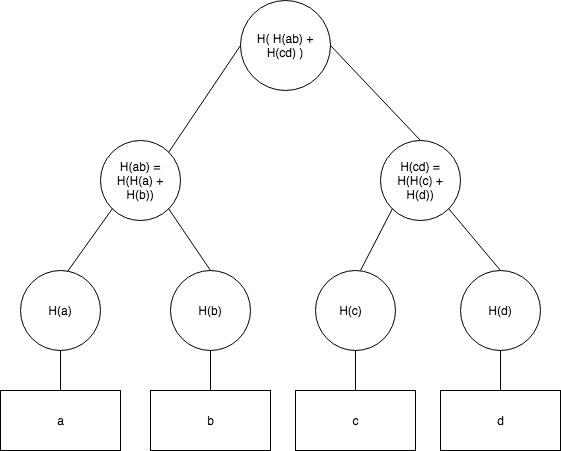
\includegraphics[width=0.7\textwidth]{radixTree}
    \caption{Esempio di Merkle Patricia Tree}
\end{figure}


La prima applicazione del Merkle Proof è stata quella di Bitcoin che ha adottato questo meccanismo per inserire all'interno dei blocchi l'hash del nodo root del Merkle tree con le transazioni. 
Il Merkle Tree utilizzato da Bitcoin era però troppo limitato per poter essere utilizzato anche in Ethereum che quindi ora utilizza una implementazione leggermente differente denominata Merkle Patricia tree.
I Merkle Patricia tree sono deterministici, se ne creiamo due con le stesse coppia chiave-valore otterremo due strutture identiche, inoltre garantiscono inserzione, ricerca ed eliminazione in O(log(n)).
Un miglioramento introdotto in questa implementazione riguarda la sicurezza, ogni nodo infatti viene identificato tramite un hash, in questo modo il nodo root diventa una firma dell'intera struttura dati e possiamo subito capire se ci sono state modifiche al blocco originale.
\begin{figure}[H]
    \centering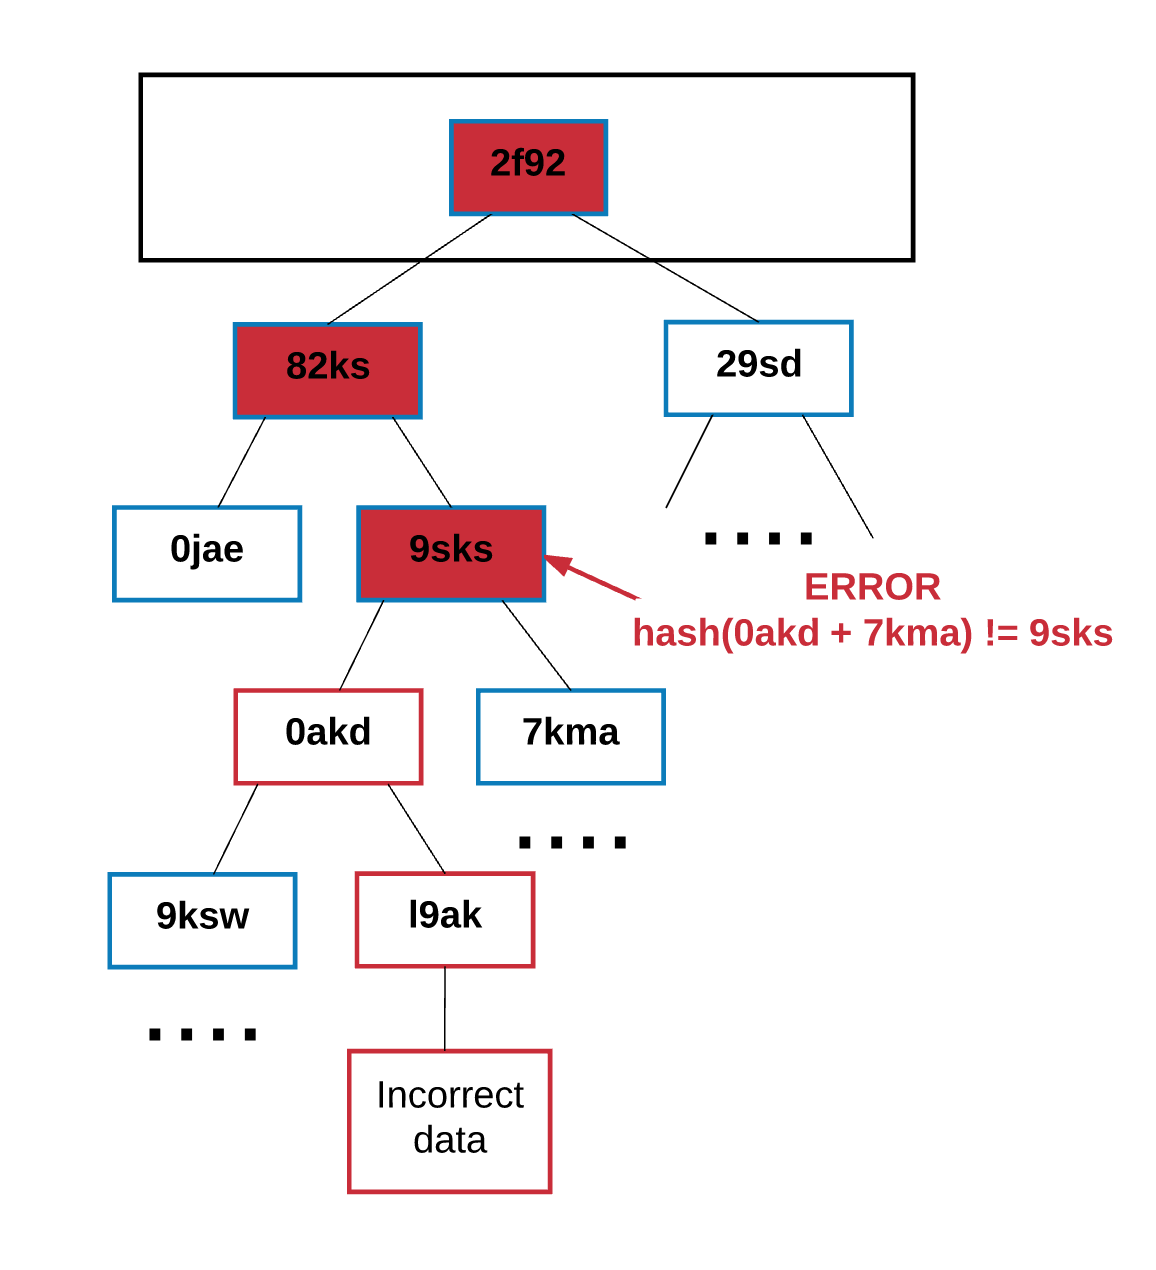
\includegraphics[width=0.7\textwidth]{MerkleTreeError}
    \caption{Verifica delle veridicità dei dati estratti dal Merkle Patricia Tree}
\end{figure}


Per migliorare l'efficienza di un Merkle Patricia Tree sono stati introdotti vari tipi di nodi:

\begin{itemize}
\item Nodo vuoto;
\item Foglia: rappresentata da un array, un elemento è il path del nodo e uno è il valore corrispondente. Ad esempio: creiamo un albero vuoto e inseriamo un unico elemento, questo sarà quindi posizionato come nodo root e avremo solamente una associazione (chiave, valore) al suo interno;

\begin{figure}[H]
    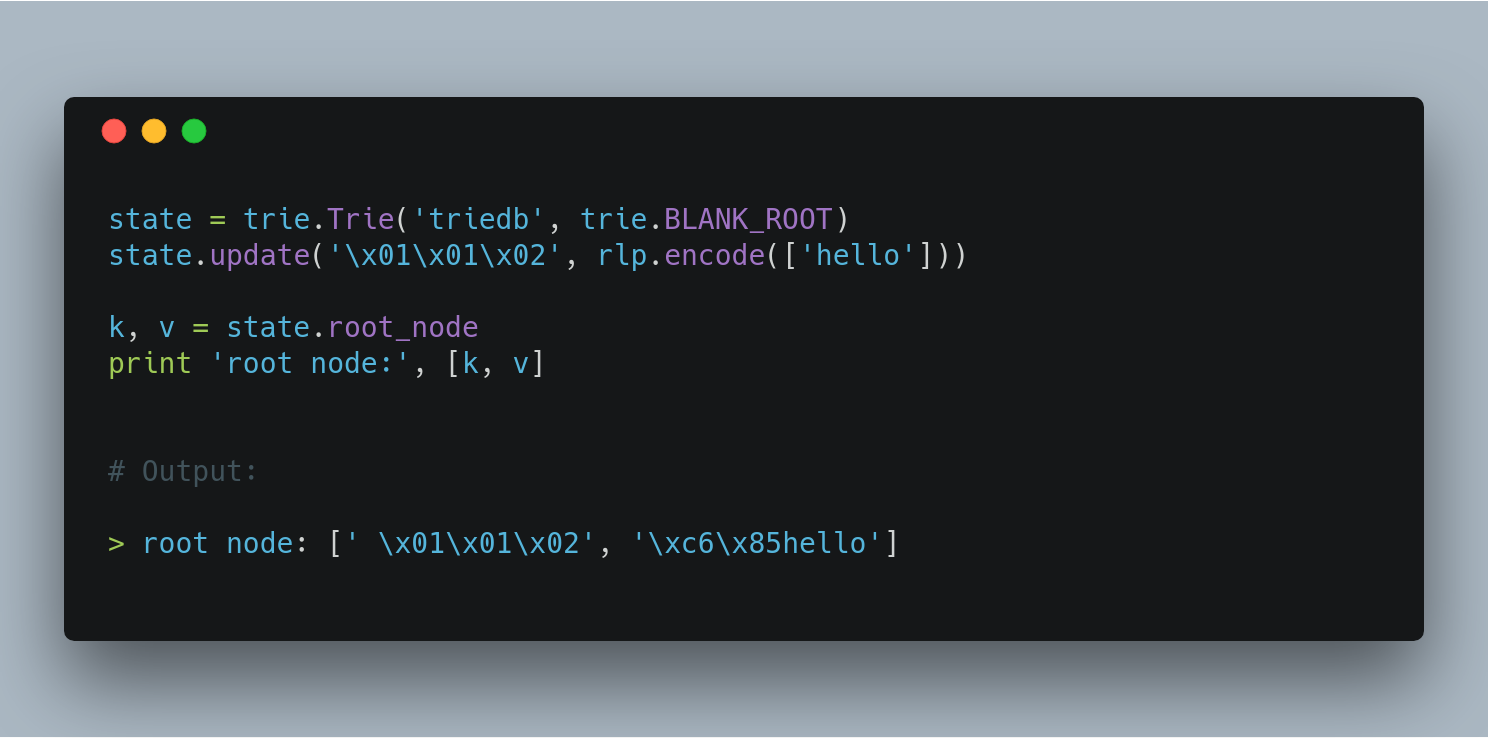
\includegraphics[width=\textwidth]{carbon-11}
    \caption{Esempio di nodo foglia}
\end{figure}
\item Branch Nodes: array di 17 elementi, 16 corrispondono ai possibili caratteri hex presenti in una chiave e ci permettono di rappresentare gli eventuali figli del nodo, 1 elemento invece serve per contenere il valore del nodo.

\begin{figure}[H]
    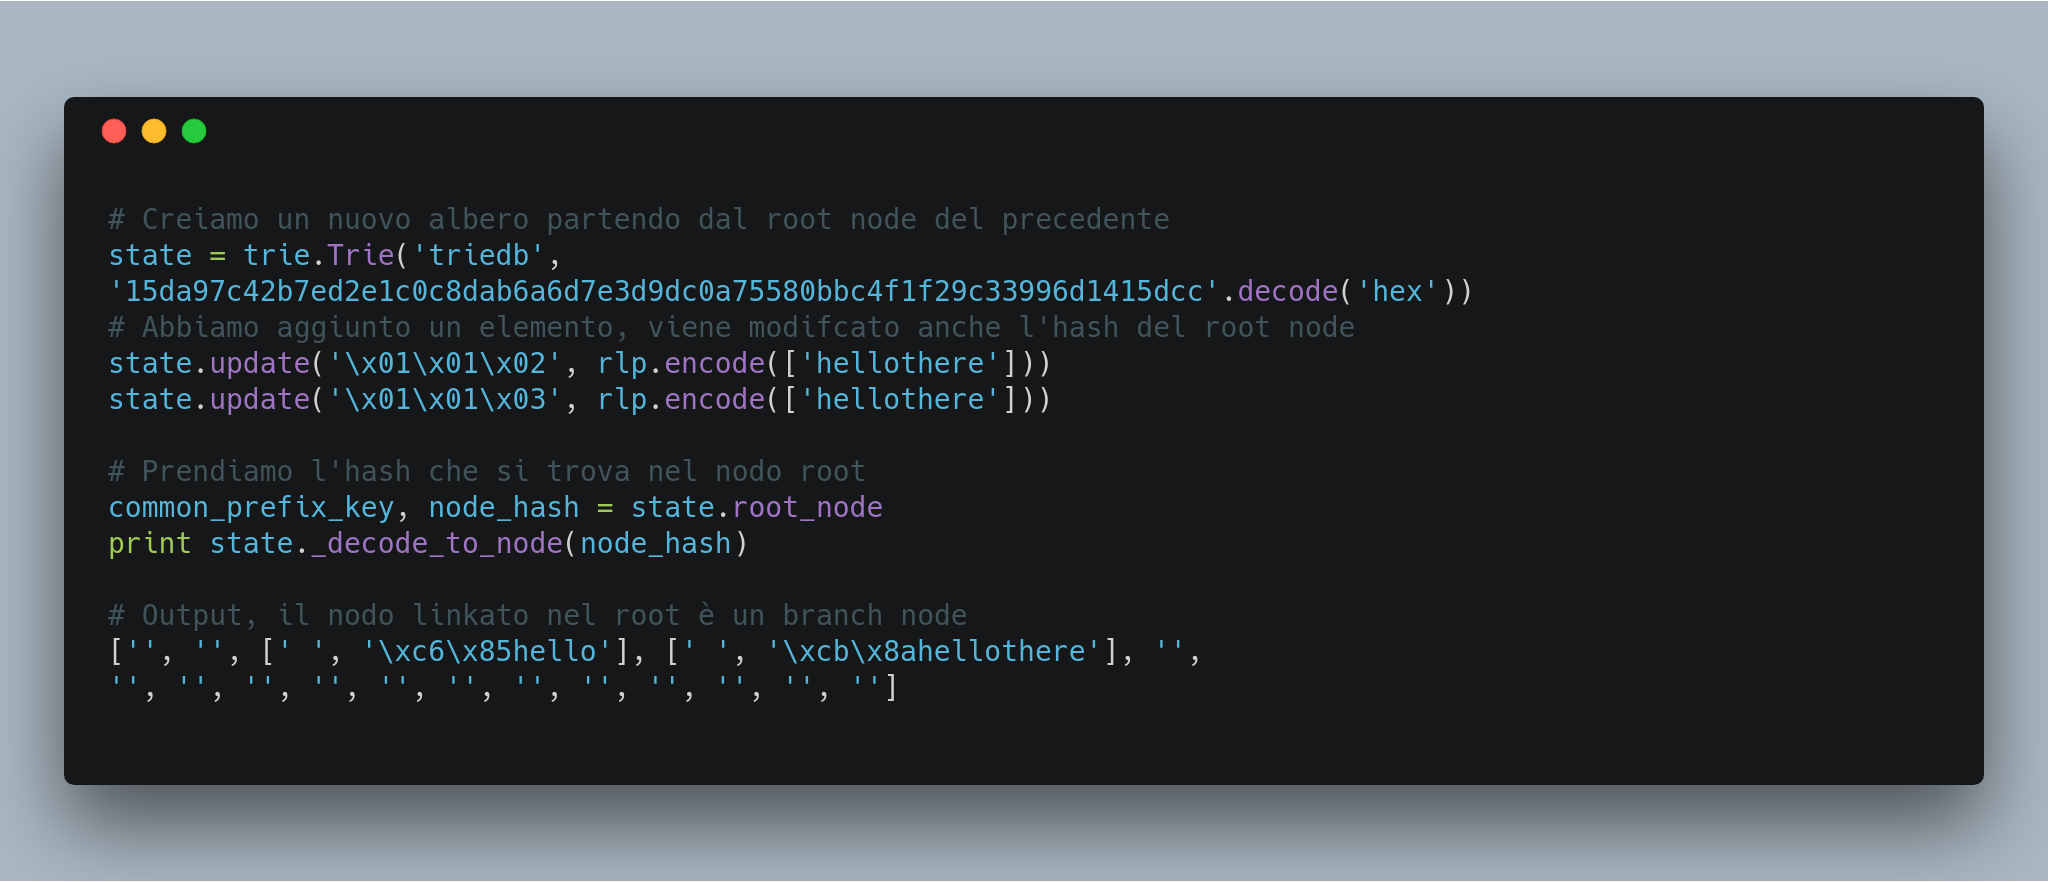
\includegraphics[width=\textwidth]{carbon-13}
    \caption{Esempio di nodo branch}
\end{figure}

Possiamo fare un esempio di Merkle Patricia Tree con un branch node, prendiamo un albero in cui inseriamo due elementi, 1000 e 2000 con chiavi rispettivamente 0xBEA e 0xBEE. 
Avremo un nodo root in cui inseriremo solamente la chiave OxBE e poi i 16 figli, i due che ci interessano in particolare sono quelli con i valori 1000 e 2000 e vengono identificati perchè avranno come chiave 0xA e 0xE. 
Quindi se vogliamo ricercare nell'albero il valore identificato dalla chiave 0xBEE, seguiremo nell'albero il percorso e troveremo il valore 2000;

\begin{figure}[H]
    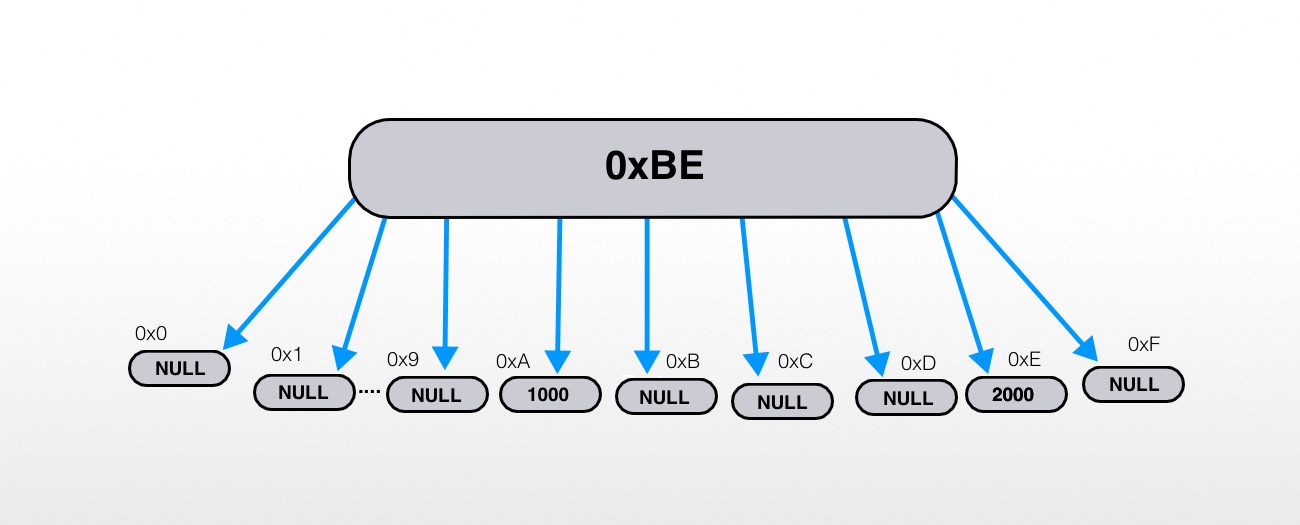
\includegraphics[width=\textwidth]{MMPT.jpg}
    \caption{Esempio di un Merkle Patricia Tree con nodo branch}
\end{figure}

\item Extension nodes: questo tipo di nodo è una ottimizzazione del Branch Node. L'extension node viene utilizzato quando il branch node ha solamente un figlio, in questo caso viene utilizzato un array di 2 elementi, uno è il path del nodo corrente e uno l'hash del figlio. Dato che anche la foglia è un array di due elementi, è stato necessario aggiungere un prefisso nel path per fare una distinzione, nella foglia abbiamo ``0x20`` o ``0x3``, nell'extension node invece ``0x00`` o ``0x1``.

\begin{figure}[H]
    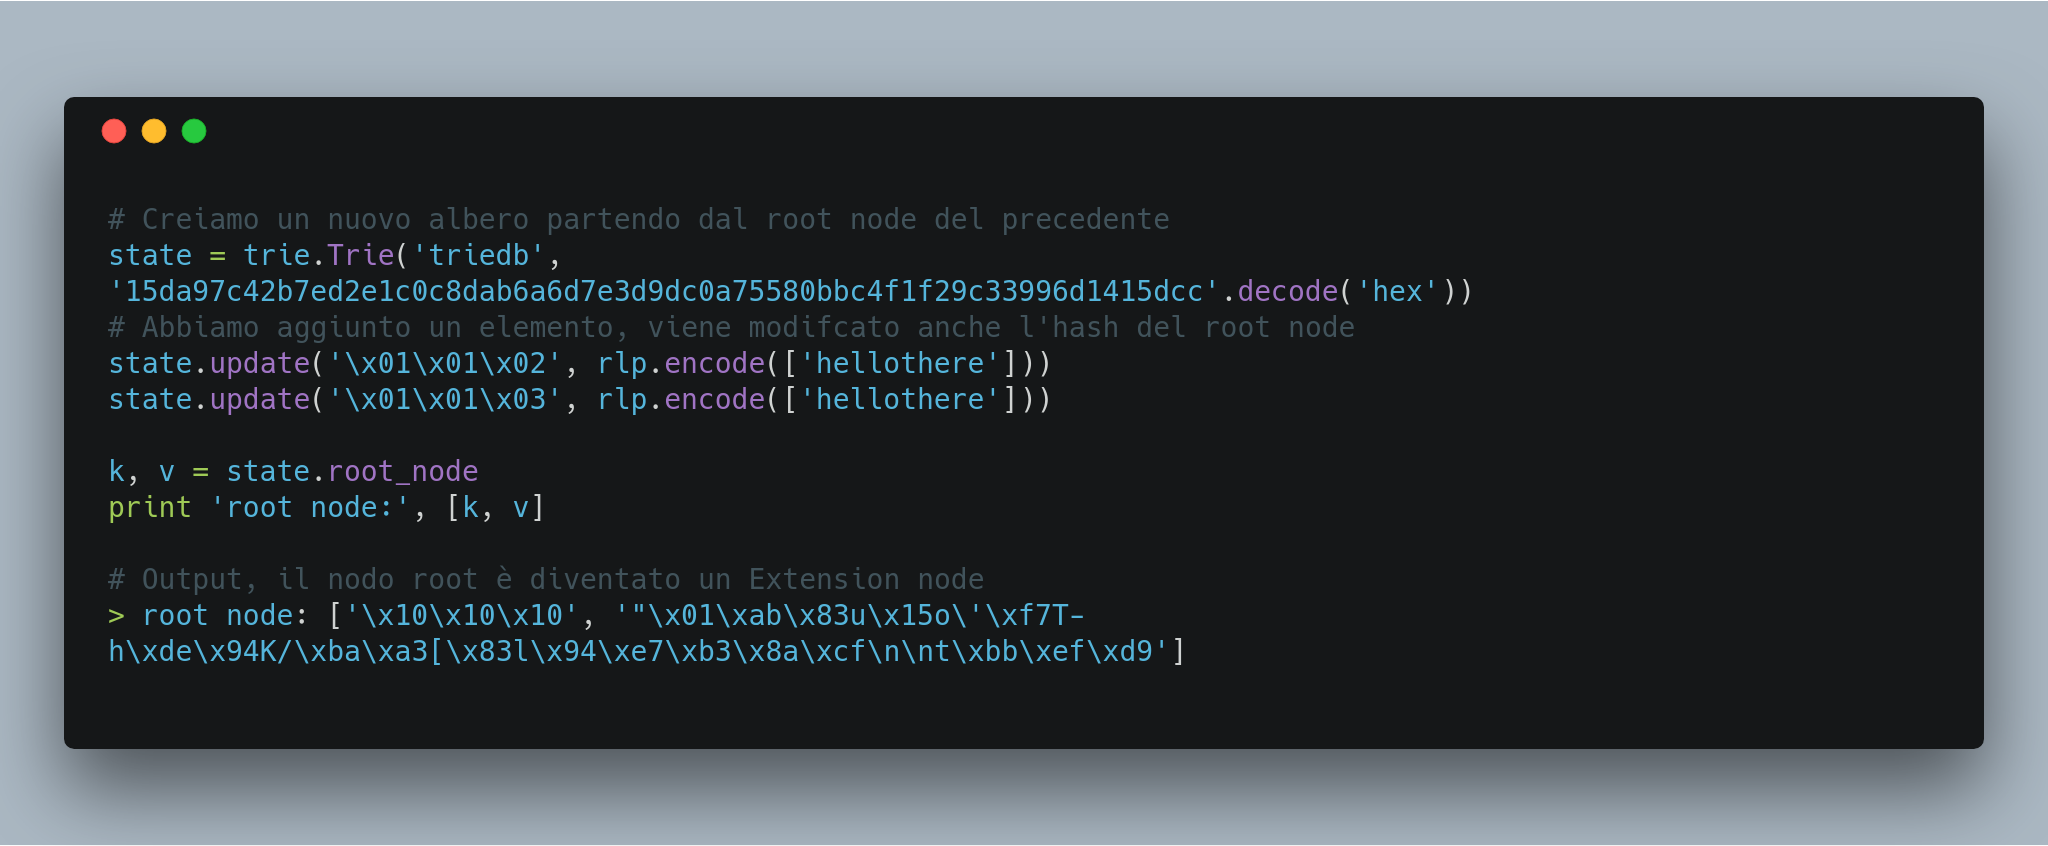
\includegraphics[width=\textwidth]{carbon-12}
    \caption{Esempio di nodo Extension}
\end{figure}

\end{itemize}

I blocchi di Ethereum, come abbiamo già visto, contengono 3 Merkle Patricia Tree, uno per le transazioni, uno per i receipt e uno per lo stato complessivo della blockchain. Quando poi un utente richiede le transazioni di un determinato blocco, queste vengono trasformate dall'albero in una lista e vengono inviate. 
Lo stesso utente potrà poi controllare che le transazioni ricevute siano effettivamente quelle presenti nella blockchain andando a ricostruire l'albero e controllando che l'hash del nodo root sia lo stesso che troviamo nel blocco.
Nell'albero che utilizziamo per memorizzare lo stato, il percorso è determinato dall'indirizzo degli account mentre il valore corrispondente è la tuple $<nonce, ether disponibili, storageRoot, codeHash>$. Questo albero subisce modifiche costanti ogni volta che viene aggiunto un nuovo blocco all'interno della blockchain.
L'albero delle transazioni invece è unico per ogni blocco e non viene mai modificato, utilizziamo l'indice della transazione per muoverci al suo interno e il valore che troviamo nelle foglie corrisponde ai dettagli della transazione.
Anche l'albero dei receipt è unico per ogni blocco e una volta creato non viene più modificato, utilizziamo l'indice della transazione per muoverci al suo interno e nelle foglie troviamo i dettagli del receipt.

\newpage
\section{Parsing della blockchain}

\subsection {Sviluppo di un parser in Java}

Il tirocinio svolto ha lo scopo di parsare il contenuto della blockchain di Ethereum estraendo le transazioni presenti al suo interno per poi creare un grafo che le rappresenti.
L'idea iniziale del tirocinio è stata quella di scrivere un parser in Java che potesse svolgere in automatico tutto il lavoro di estrazione delle informazioni.
Il parser prende in input un file di testo esadecimale contenente uno dopo l'altro tutti i blocchi presenti nella blockchain, codificati nel formato RLP, e successivamente estrae le informazioni utili. Il file nominato poco sopra è di dimensioni piuttosto elevate dato che il contenuto della blockchain supera i 600GB di spazio occupato.

Per realizzare il parsing abbiamo sfruttato le regole di codifica di RLP elencate in precedenza andando a suddividere il file in blocchi basandoci sulla lunghezza in byte del blocco stesso.

Una volta individuato un singolo blocco, è stato necessario reperire una libreria che ci permettesse di suddividere la stringa estratta e codificata tramite RLP, in modo da evitare di svolgere manualmente questo procedimento.
Abbiamo scelto la libreria EthereumJ \cite{EthereumJ}, disponibile su GitHub e descritta nel paragrafo 4.3.
Questa libreria permette di decodificare una stringa RLP andando ad estrarre le informazioni che ci interessano, ad esempio nel caso di un blocco è stata scritta una funzione per il parsing, la parte più importante è riportata nella Figura 5.20:

\begin{figure}[H]
    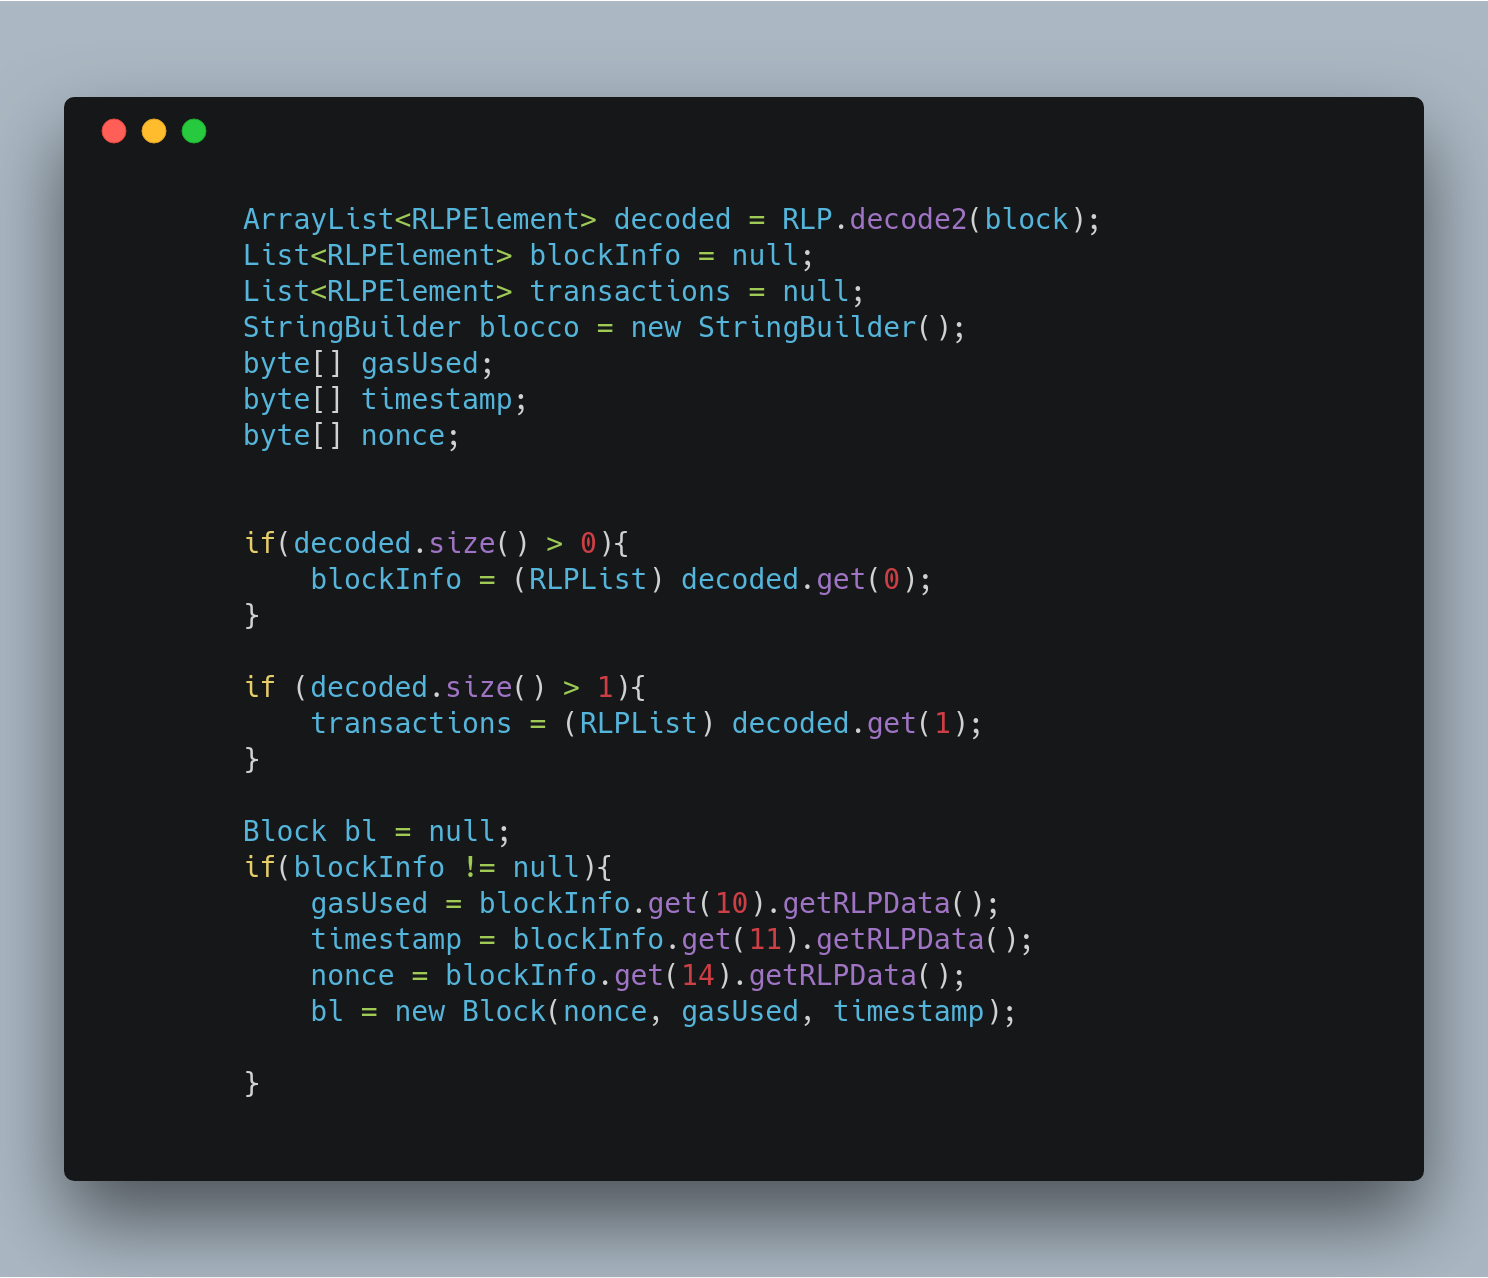
\includegraphics[width=\textwidth]{carbon-14}
    \caption{Parsing di un blocco}
\end{figure}


Per prima cosa la stringa viene decodificata (funzione decode2), il valore restituito viene inserito in un ArrayList che può avere un singolo elemento contenente i dettagli del blocco, quando non sono presenti transazioni. Se invece è presente un numero maggiore di elementi nell'array, vuol dire che all'interno del blocco sono presenti anche delle transazioni che devono essere parsate.
Nell'ultima parte del codice andiamo poi ad estrarre dalla lista di RLP i vari campi del blocco che ci interessano, in questo caso il gasUsed, il timestamp e il nonce.

Per quanto riguarda il parsing delle transazioni, il discorso è più complicato, alcuni dei campi contenuti all'interno della stringa possono essere estratti facilmente utilizzando la stessa libreria utilizzata per i blocchi, in altri casi invece, occorre effettuare dei calcoli che sono risultati abbastanza pesanti.\newline
Nella prima parte dell'estrazione delle informazioni di una transazione è possibile usare la libreria citata in precedenza, come mostrato nell'immagine:
\begin{figure}[H]
    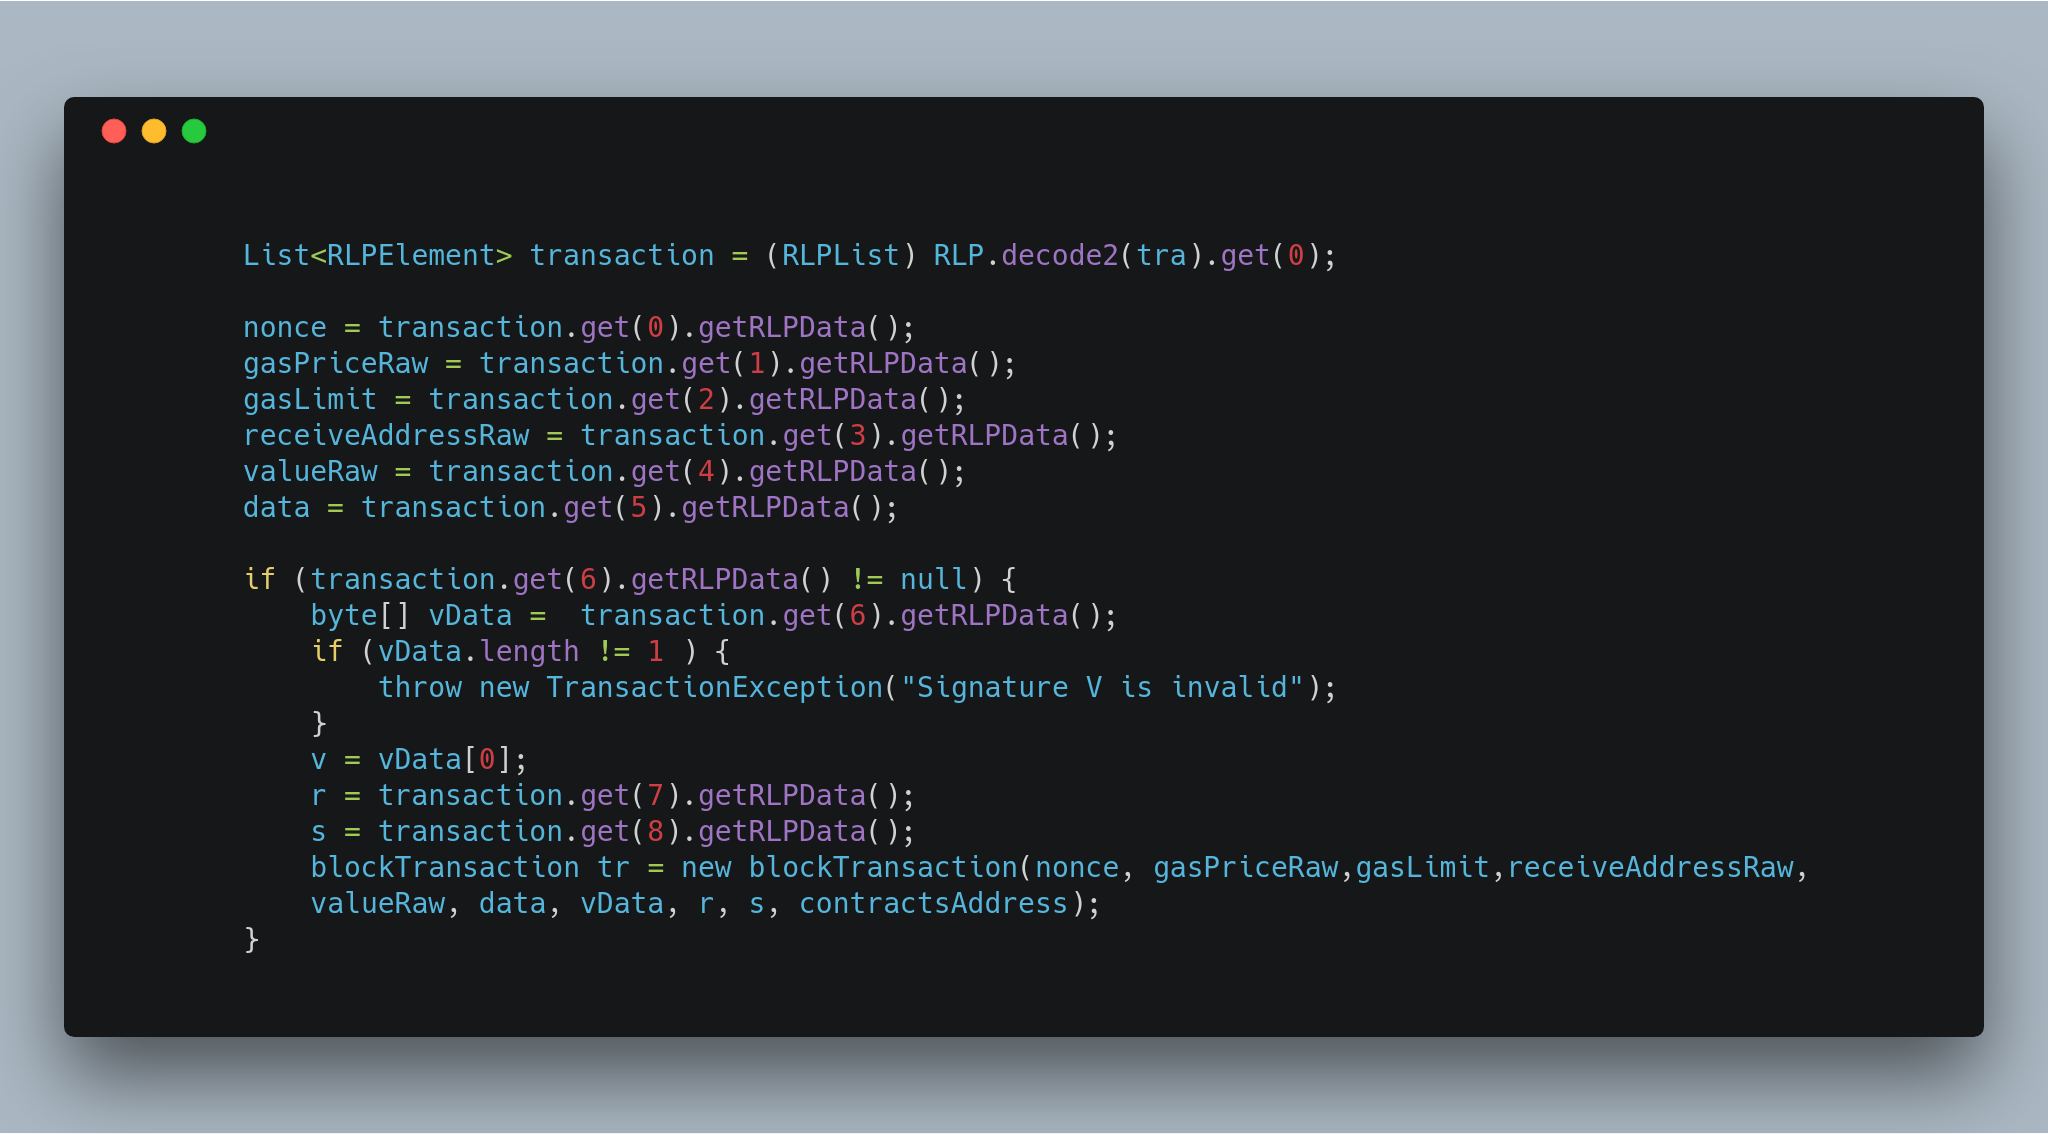
\includegraphics[width=\textwidth]{carbon-15}
    \caption{Parsing di una transazione}
\end{figure}
La parte più complicata riguarda il calcolo del mittente della transazione e l'indirizzo del contratto, qualora la transazione sia una richiesta di creazione di uno smart contract.
Come già detto nel paragrafo 5.3 ,in cui abbiamo parlato dei campi di una transazione, il mittente di quest'ultima non viene inserito nella richiesta che viene inviata in rete, semplicemente perché è possibile ricavarlo partendo dalla firma che viene messa sulla transazione.
Il problema in questo caso è però rappresentato dal procedimento necessario per eseguire questa operazione, va infatti calcolato un hash su alcuni campi della transazione, escludendo quelli che non danno vita alla firma e successivamente si utilizza la crittografia su curve ellittiche per ricavare l'indirizzo del mittente sfruttando l'hash e una firma che possiamo ottenere dai campi v, r, s. Questi tre campi, come indicato nel paragrafo 5.3 rappresentano la firma della transazione. 
Questo procedimento si è rivelato piuttosto pesante nella pratica.

\begin{figure}[H]
    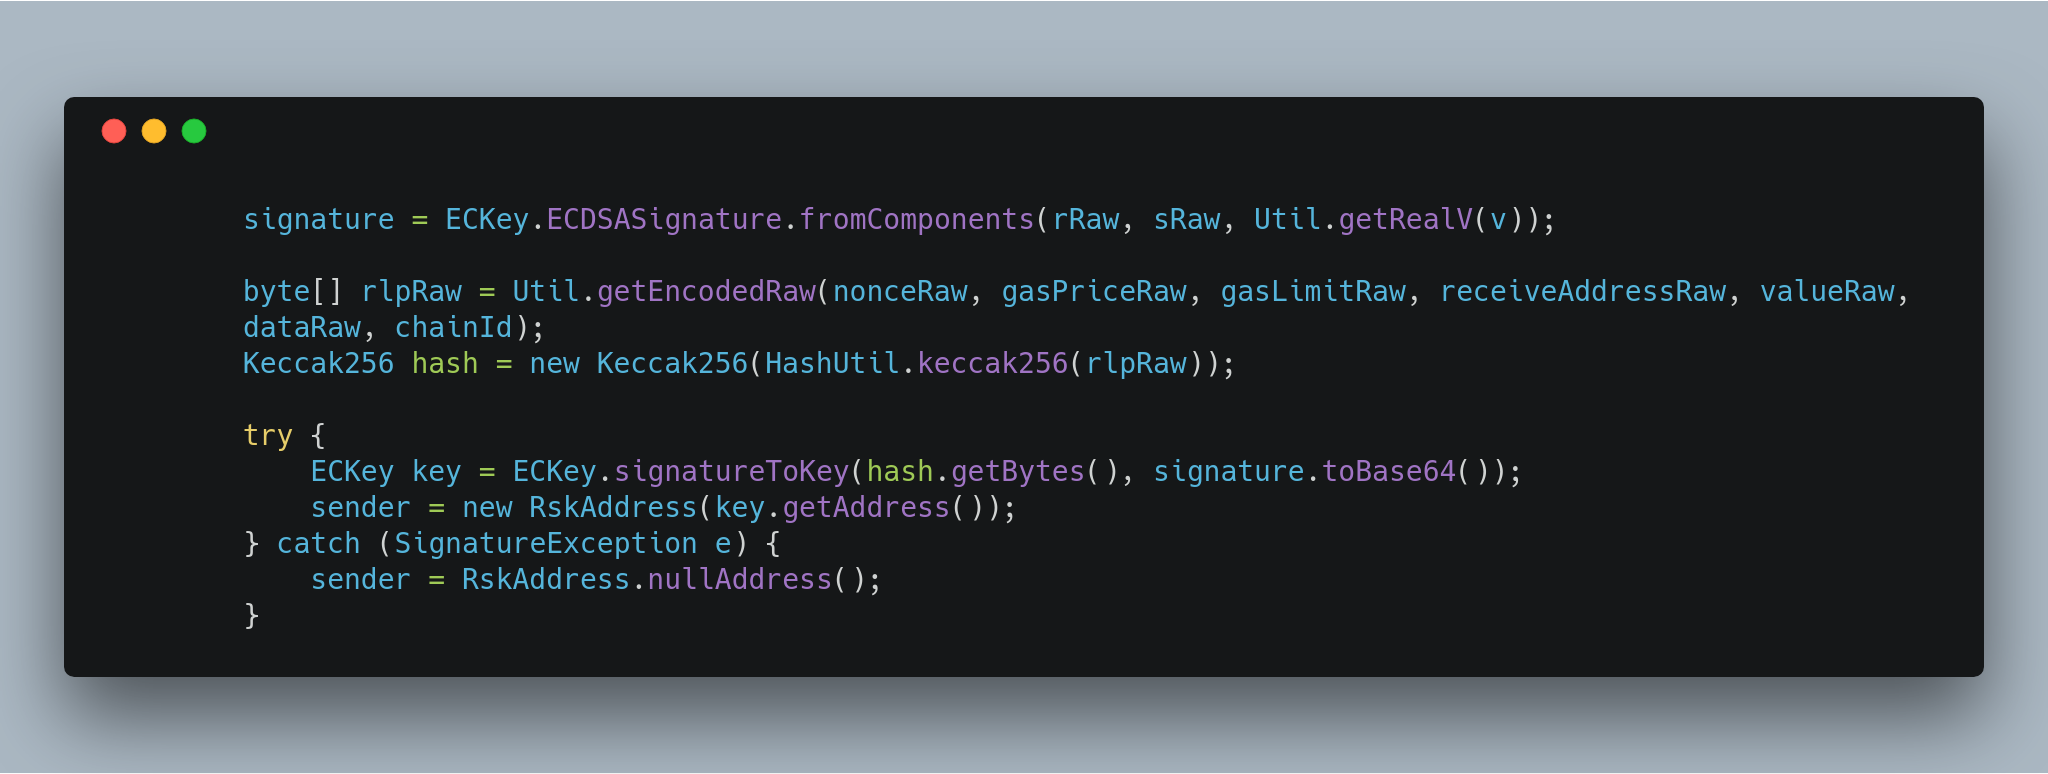
\includegraphics[width=\textwidth]{carbon-16}
    \caption{Estrazione del mittente di una transazione}
\end{figure}

Il secondo problema è legato invece alle transazioni di creazione di un nuovo smart contract, da queste dovevamo ottenere l'indirizzo del contratto appena creato. Questo indirizzo è disponibile nel receipt della transazione che, sfortunatamente, non era in nostro possesso.
Studiando lo Yellow Paper abbiamo poi capito che questa informazione può essere generata in modo deterministico partendo dal mittente che chiede la creazione del contratto e dal suo nonce.
\begin{figure}[H]
    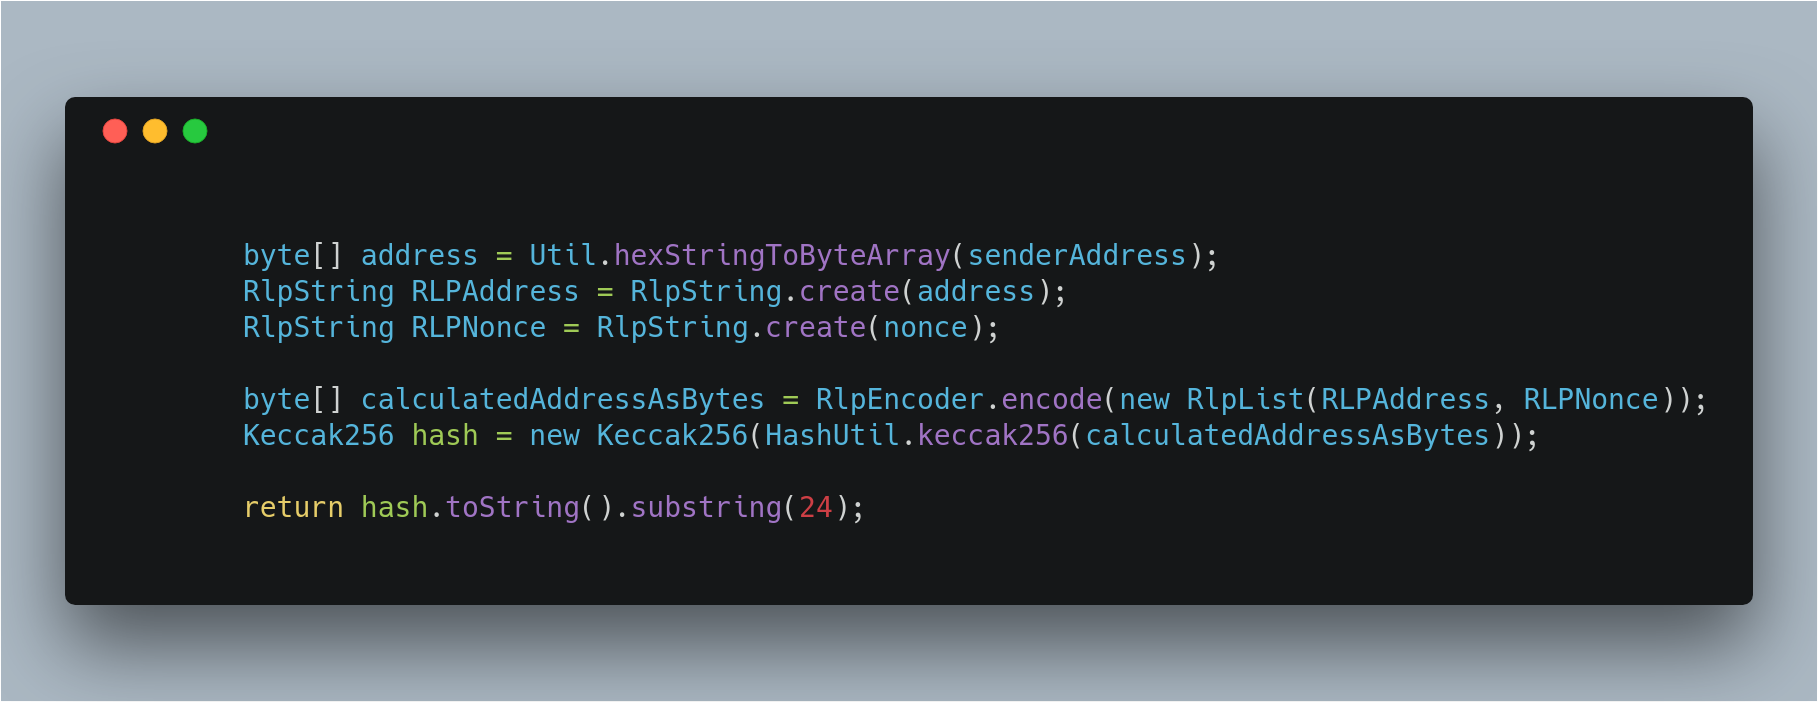
\includegraphics[width=\textwidth]{carbon-17}
    \caption{Estrazione dell'indirizzo del contratto}
\end{figure}

Il calcolo dell'indirizzo del contratto richiede un array di byte in cui vengono codificate le due informazioni citate in precedenza ovvero indirizzo del mittente e nonce.
Calcolando poi l'hash dell'array di byte e prendendo solamente gli ultimi 160-bit della stringa risultante si ottiene l'indirizzo cercato.
Anche in questo caso si è presentato lo stesso problema avuto con il mittente e pertanto questo procedimento si è rivelato computazionalmente costoso.

Una volta completata la scrittura di questo parser, sono stati effettuati alcuni test prima con file di testo di piccole dimensioni e con pochi blocchi, per poi passare a file sempre più grandi.
Il problema principale era legato al tempo necessario per elaborare tutto il file e calcolare le informazioni non riportate in modo esplicito (indirizzo del mittente e del contratto nel caso di creazione di un nuovo contratto).

\begin{figure}[H]
    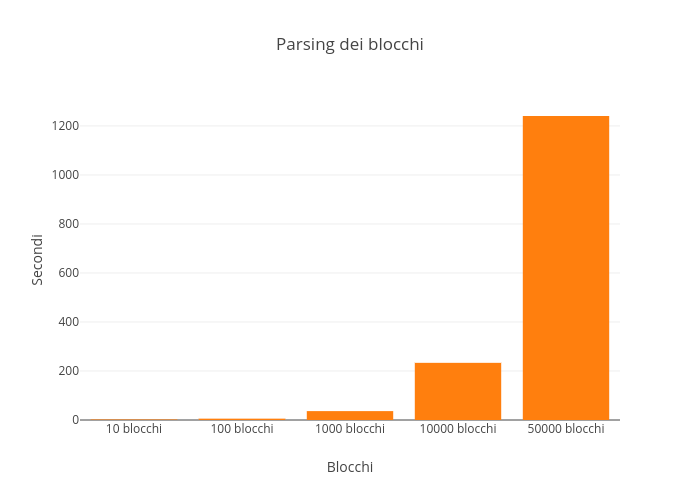
\includegraphics[width=\textwidth]{Plot1.png}
    \caption{Performance del parser single Thread}
\end{figure}

La prima idea è stata quella di rendere il parser multithread ma ci siamo subito scontrati con una problematica, nel file di output generato dal parser, i blocchi sarebbero dovuti essere ordinati in base alla loro creazione. Utilizzando un sistema multithread in modo banale che andasse a parsare più blocchi contemporaneamente in thread differenti non sarebbe stato possibile mantenere l'ordine.
Perdere l'ordinamento sarebbe stato un problema per capire quali transazioni fossero state eseguite verso un contratto e quali verso un utente esterno. L'idea infatti era quella di mantenere in memoria gli indirizzi dei contratti in modo da poter fare la differenziazione delle transazioni in modo rapido. Il problema però era che senza mantenere l'ordine sarebbe stato possibile processare una transazione verso un contratto senza prima aver elaborato la creazione del contratto stesso, questo avrebbe comportato una errata identificazione del tipo della transazione.
Questa è stata la motivazione per cui non è stato neanche possibile parsare le transazioni e poi ordinarle in un secondo momento.
\newline
Per implementare il multithread quindi abbiamo suddiviso il parser in questo modo, un Thread principale si sarebbe occupato della lettura dei dati dal file di testo e avrebbe eseguito un numero minimo di calcoli, tra cui anche l'estrazione dell'indirizzo dello smart contract nel caso di una transazione con una richiesta di creazione del contratto.
Poi un pool di Thread invece avrebbe svolto le operazioni più pesanti, come l'estrazione del mittente della transazione.
La comunicazione tra i thread avviene con il supporto di una coda di blocchi.

\begin{figure}[H]
    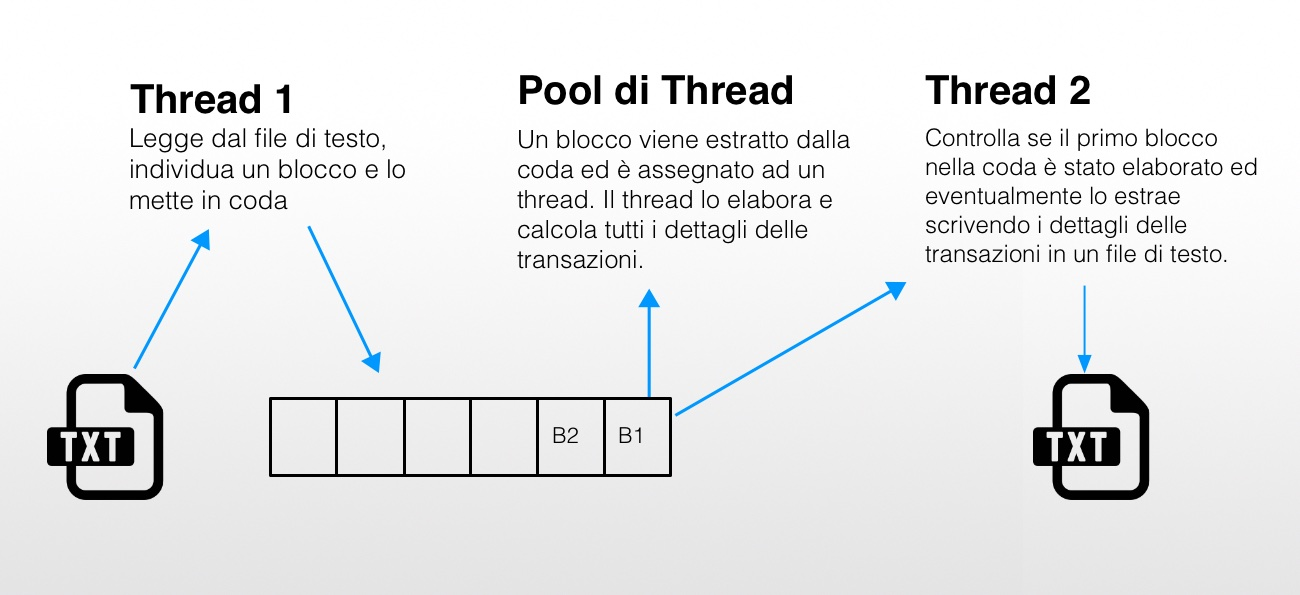
\includegraphics[width=\textwidth]{Thread.jpg}
    \caption{Organizzazione dei thread nel parser scritto in Java}
\end{figure}

Quando viene inserito un nuovo blocco nella coda, un Thread del pool prende questo blocco e fa tutti i calcoli necessari per calcolare il mittente o l'indirizzo del contratto ed alla fine setta un flag che permette di capire se per quel blocco la computazione è stata effettuata oppure no.
Nella coda potrei quindi avere ad esempio un primo elemento su cui un thread sta lavorando e un secondo che invece è già stato elaborato.
Sarà poi un terzo Thread a controllare il primo elemento della coda, se questo è stato elaborato, lo stesso Thread si occupa anche di andare a scrivere il blocco nel file di output e poi lo elimina dalla coda andando a controllare quello che ora sarà stato spostato in prima posizione.
In questo modo verrà mantenuto l'ordine ma la computazione più pesante verrà svolta in contemporanea andando quindi a risparmiare del tempo.
Stando alle prove svolte, introdurre questo pool di Thread ha comportato un miglioramento delle prestazioni abbassando di molto il tempo necessario per parsare i blocchi.

\begin{figure}[H]
    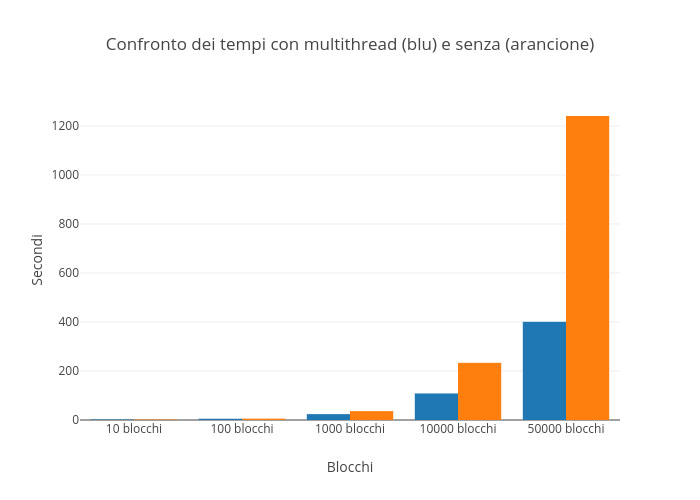
\includegraphics[width=0.95\textwidth]{Plot2.jpg}
    \caption{Confronto delle performance del parser single thread con quelle della versione multi thread}
\end{figure}


Nonostante l'introduzione del multithread e il miglioramento delle prestazioni, il tempo necessario per il parsing risulta ancora piuttosto alto.
\newline
Si è poi presentato immediatamente un altro problema: per tutte le transazioni estratte dai blocchi era necessario capire se queste fossero fallite oppure no in modo da non inserire all'interno del grafo le transazioni non andate a buon fine.
L'idea inizialmente è stata quella di ovviare al problema andando a controllare che il gas utilizzato per lo svolgimento della transazione fosse minore del gas massimo disponibile, questo però non è stato possibile per due ragioni. La prima è legata al fatto che il campo gasUsed è presente nel receipt della transazione e non avevamo a disposizione il receipt. La seconda è che controllando questi due valori e verificandone l'uguaglianza avremmo scartato troppe transazioni andate a buon fine che utilizzavano tutto il gas a loro disposizione. 
\newline
Abbiamo cercato di stimare il tempo necessario per parsare tutta la blockchain utilizzando il parser scritto in Java, la versione single thread avrebbe elaborato il contenuto della blockain in circa 150 giorni quindi un tempo esageratamente troppo elevato.
Con la versione multi Thread invece sarebbero stati necessari circa 20 giorni per il parsing completo.
Nonostante questa stima abbiamo cercato una seconda soluzione alternativa per eseguire il parsing, considerato soprattutto il fatto che con quella appena descritta non sarebbe stato possibile estrarre lo status delle transazioni.

\subsection {Uso di Geth per il parsing di blocchi e transazioni}

Nel capitolo 4.1 abbiamo parlato di Geth evidenziandone il funzionamento generale e soffermandoci in particolare sulla sincronizzazione della blockchain di Ethereum. Questo procedimento di sincronizzazione ha richiesto svariate ore di lavoro per scaricare in locale più di 300Gb di dati.
Una volta eseguita la sincronizzazione della blockchain, siamo passati alla fase di estrazione dei dati, in particolare abbiamo estrapolato da ogni blocco tutte le transazioni contenute al suo interno.
I dati estratti dalla blockchain sono stati salvati in un file di testo, inserendo in ogni riga una transazione con le seguenti informazioni:
\begin{itemize}
\item Blocco di appartenenza;
\item Nonce;
\item Timestamp;
\item Hash della transazione;
\item Mittente;
\item Destinatario;
\item Indirizzo del contratto (null nel caso in cui nella transazione non si fosse creato un contratto);
\item Valore scambiato;
\item Gas Limit;
\item Gas Utilizzato;
\item Status della transazione (0 in caso di fallimento, 1 altrimenti);
\item Input.
\end{itemize}

Per l'estrazione è stato scritto uno script in Javascript poi eseguito tramite la console di Geth salvando l'output su file.
Lo script scandisce tutti i blocchi presenti nella blockchain, grazie alla libreria Web3JS e alla funzione getBlock recupera per ognuno di essi il timestamp e lista delle transazioni presenti all'interno del blocco.

\begin{figure}[H]
    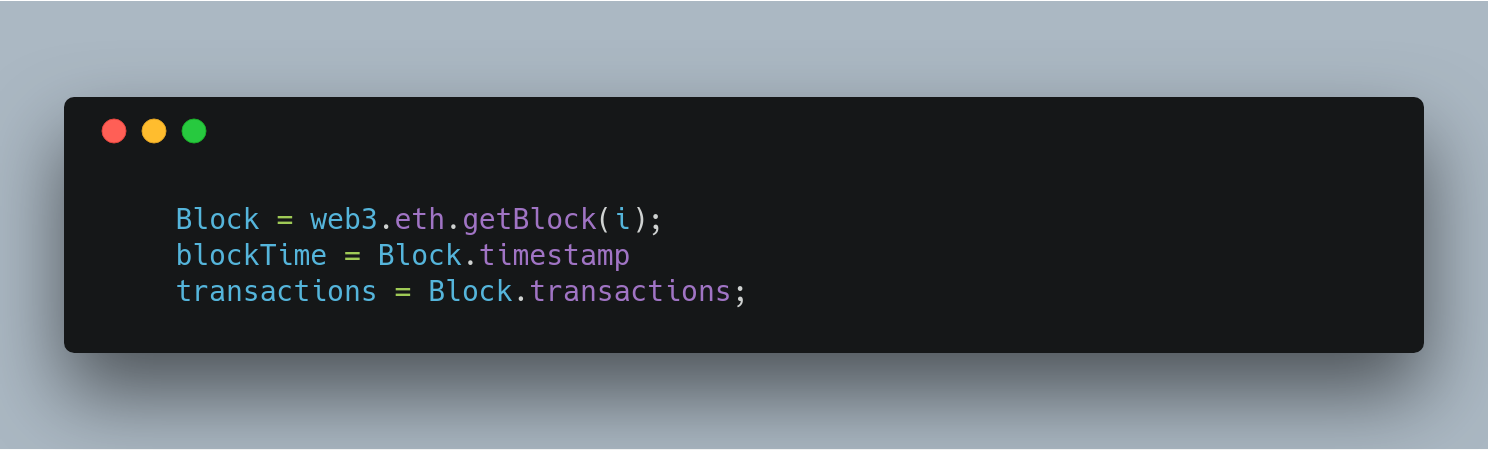
\includegraphics[width=\textwidth]{carbon-19}
    \caption{Estrazione di un blocco}
\end{figure}

All'interno della lista, ogni transazione è identificabile mediante un hash, questa informazione ci ha consentito di utilizzare anche in questo caso Web3JS per estrarre tutti i dati necessari.
In particolare per tutte le transazioni abbiamo usato le richieste getTransactionReceipt e getTransaction di Web3, passando come parametro l'hash, per ottenere i dettagli della transazione e il receipt.
Una volta memorizzata la transazione o il receipt, è stato sufficiente accedere ai vari campi per poi stamparli nella console di Geth.

\begin{figure}[H]
    \centering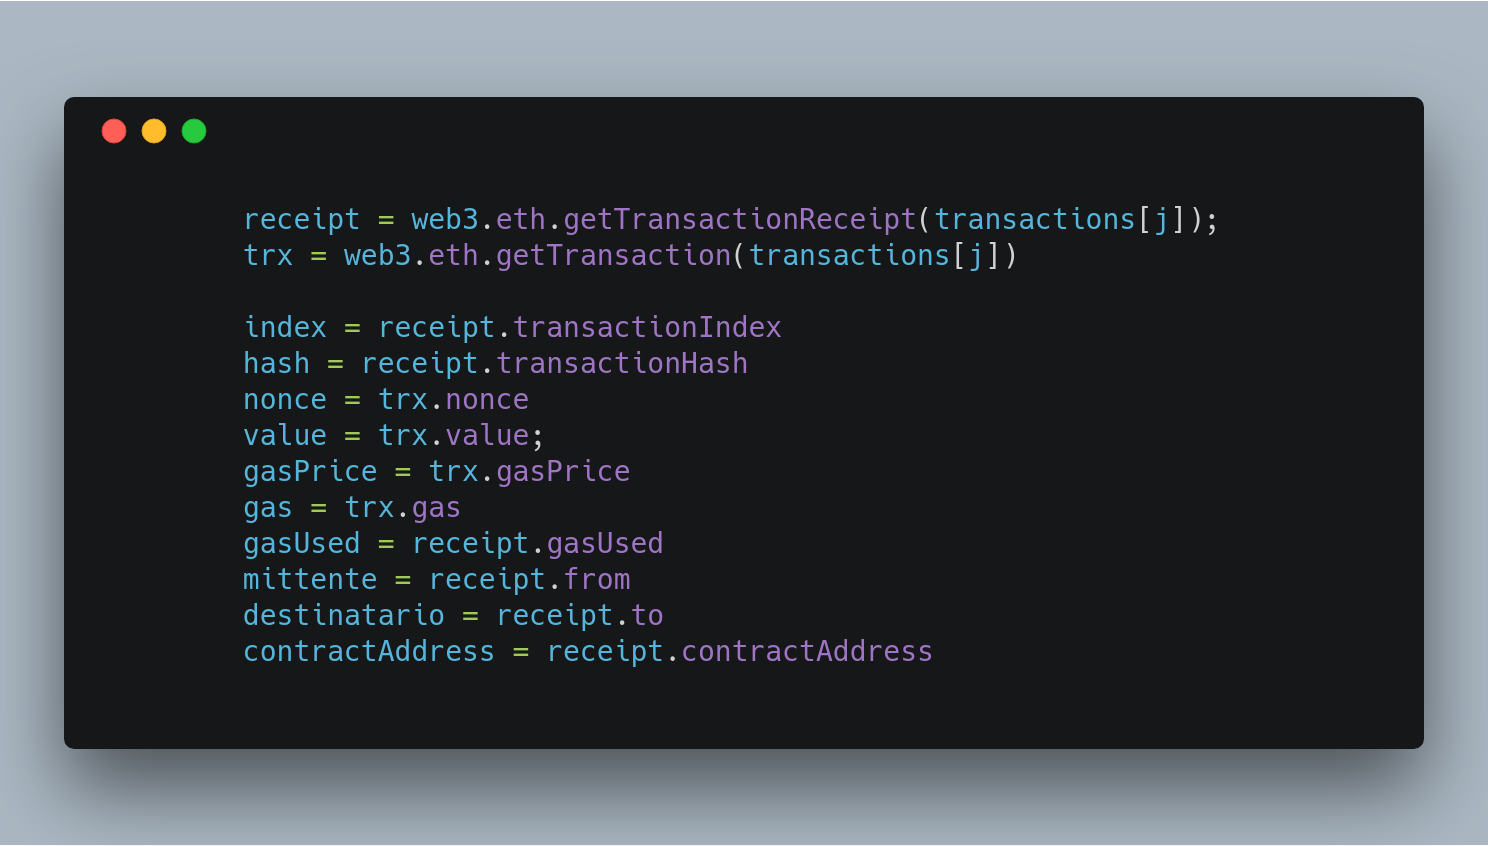
\includegraphics[width=0.9\textwidth]{carbon-20}
    \caption{Estrazione di una transazione}
\end{figure}

Per i blocchi precedenti all'hard fork Byzantium, non avendo un campo già presente nel blocco che ci indicasse lo status della transazione siamo stati obbligati ad utilizzare un metodo differente.

Inizialmente abbiamo pensato di segnare come fallite tutte le transazioni che avessero consumato tutto il gas a disposizione, banalmente potevamo semplicemente controllare se i due campi gasUsed e GasLimit fossero uguali o meno.
Purtroppo questa idea è stata subito scartata perchè ci siamo resi conto che avremmo indicate come fallite delle transazioni che in realtà erano andate a buon fine.
Fortunatamente abbiamo trovato un altro metodo utilizzabile solamente sulla blockchain sincronizzata con il flag --debug.
\newline
Dopo aver sincronizzato nuovamente la blockchain con questo flag attivo, abbiamo utilizzato le API di debug che ci hanno dato accesso a metodi non presenti in Web3JS tra cui debugTraceTransaction().
Il metodo debugTraceTransaction() permette di eseguire nuovamente la transazione desiderata così come ha fatto il miner quando l'ha inserita in un blocco e poi nella blockchain.
Per poter utilizzare questo metodo è necessario essere in possesso di tutti i dati a cui la transazione deve accedere, come ad esempio il balance e il nonce dell'utente e il bytecode del contratto nel caso di chiamata di uno smart contract.
Questo metodo ci consente di studiare tanti altri aspetti della transazione, se questa è una chiamata a contratto ci permette di comprendere tutte le operazioni che vengono svolte e quali dati sono modificati durante l'esecuzione dello smart contract.

\begin{figure}[H]
    \centering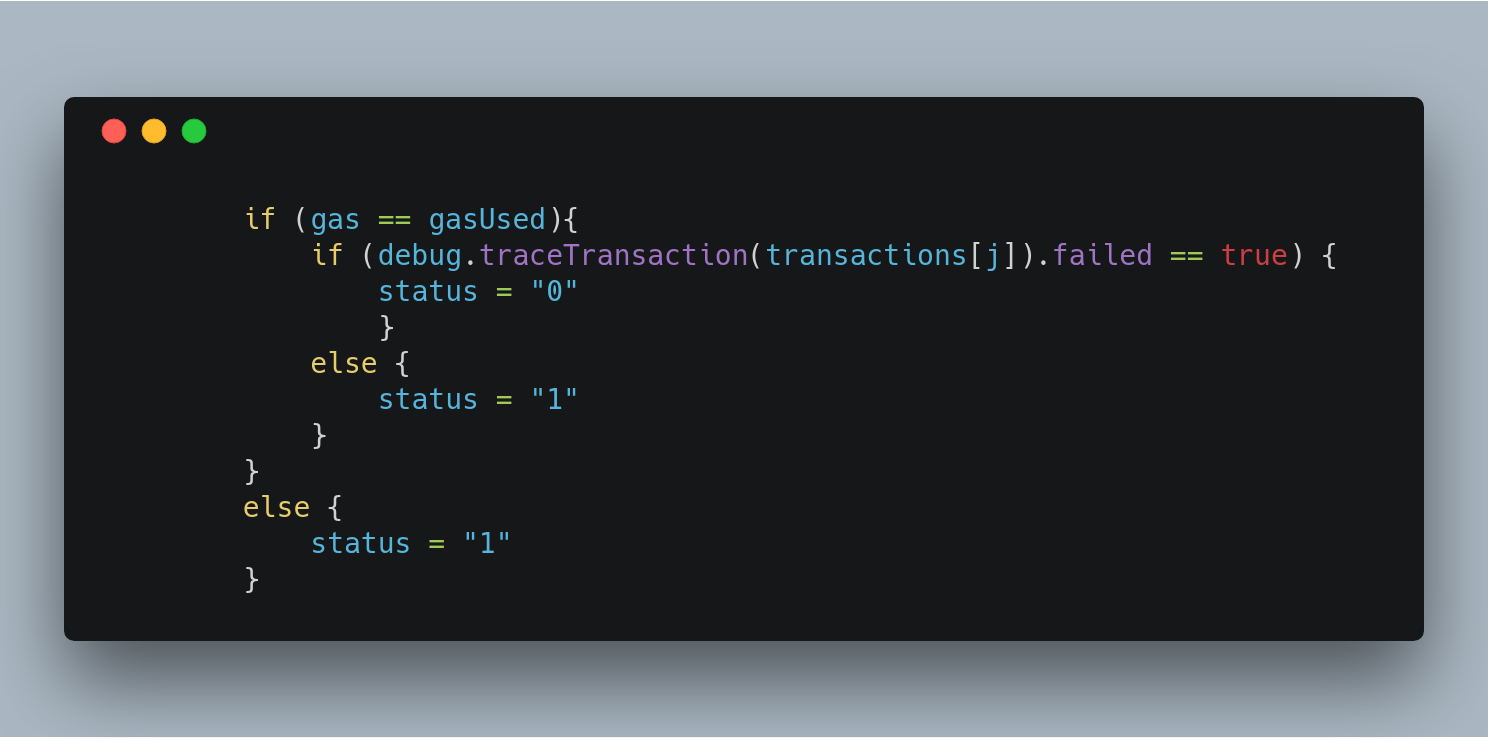
\includegraphics[width=0.95\textwidth]{carbon-21}
    \caption{Estrazione dello status di una transazione}
\end{figure}
Ovviamente l'utilizzo del debug e quindi l'esecuzione di ogni transazione presente nella blockchain che presentasse la proprietà ``gasUsed==gasLimit`` ha comportato un aumento del tempo necessario per estrarre tutti i dati. 
In particolare ci siamo trovati più volte in difficoltà con alcune transazioni verso contratti che avevano un gas consumato molto alto e che quindi richiedevano molto tempo per poter eseguire il codice dello smart contract.

\section{Costruzione del grafo Webgraph}

L'estrazione dei primi 4237648 blocchi è stata completata in circa 20 giorni, ed al termine di questa parte del lavoro abbiamo ottenuto dei file di testo contenenti le transazioni della blockchain di Ethereum nel formato scelto descritto in precedenza. 
Il tempo necessario per ottenere tutte le informazioni tramite Geth è molto simile a quello del parser scritto in Java, con il metodo utilizzato però è stato possibile ottenere anche lo status della transazione
Per passare dai dati in formato testuale al grafo in formato .webgraph sono state necessarie alcune piccole modifiche.
Per questa parte del lavoro è stato scritto un semplice parser in Java che ci ha permesso di creare alcuni file di testo aggiuntivi necessari per generare il grafo.

Abbiamo deciso di studiare il nostro dataset non solo considerando tutto l'insieme dei dati ma creando anche degli snapshot temporali ovvero dividendolo in vari dataset più piccoli contenenti le transazioni fino ad una certa data.
Quindi, partendo dal file originale con tutte le transazioni abbiamo ottenuto i seguenti file:

\begin{itemize}
    \item \textit{File Intermedio}: un file di testo ottenuto partendo dal dataset originale. Ad ogni riga corrisponde una transazione, abbiamo eliminato tutte quelle fallite e aggiunto una nuovo dato con valore 0 nel caso di una transazione da utente esterno a utente esterno, 1 nel caso di creazione di un contratto e 2 nel caso di transazione da utente esterno a contratto;
    \item \textit{Associazioni}: come descritto in precedenza, i mittenti e i destinatari di una transazione sono identificati da un indirizzo di 160 bit, dato che per creare il grafo avevamo la necessità di utilizzare dei numeri interi, è stata creata una mappatura 1:1 tra i vari indirizzi presenti nel dataset e un numero intero.
    Il formato di questo file è quindi $<Indirizzo, ID>$;
    \item \textit{ID}: questo è il file che rappesenta tutte le transazioni, contiene solamente i dati del mittente e del destinatario, come già detto non viene indicato l'indirizzo ma l'ID definito nel file con le associazioni. Il formato del file è il seguente $<IDMittente,  IDDestinatario>$;
    \item \textit{Snapshot}: abbiamo prodotto dei file di testo con lo stesso formato del file ID, questi hanno al loro interno una parte delle informazioni del file di cui abbiamo parlato in precedenza perchè consideriamo le transazioni solamente fino ad una certa data
    \item \textit{Transazioni per Tipo}: Oltre a suddividere le transazioni basandoci sul tempo, abbiamo sfruttato anche un altro dato in nostro possesso ovvero il tipo della transazione. Abbiamo quindi generato tre file nel formato $<IDMittente,\newline
    IDDestinatario>$, in ognuno di essi sono presenti solamente le transazioni del tipo scelto (creazione contratto, utente esterno-contratto, utente esterno-utente esterno).
\end{itemize}

\begin{figure}[H]
    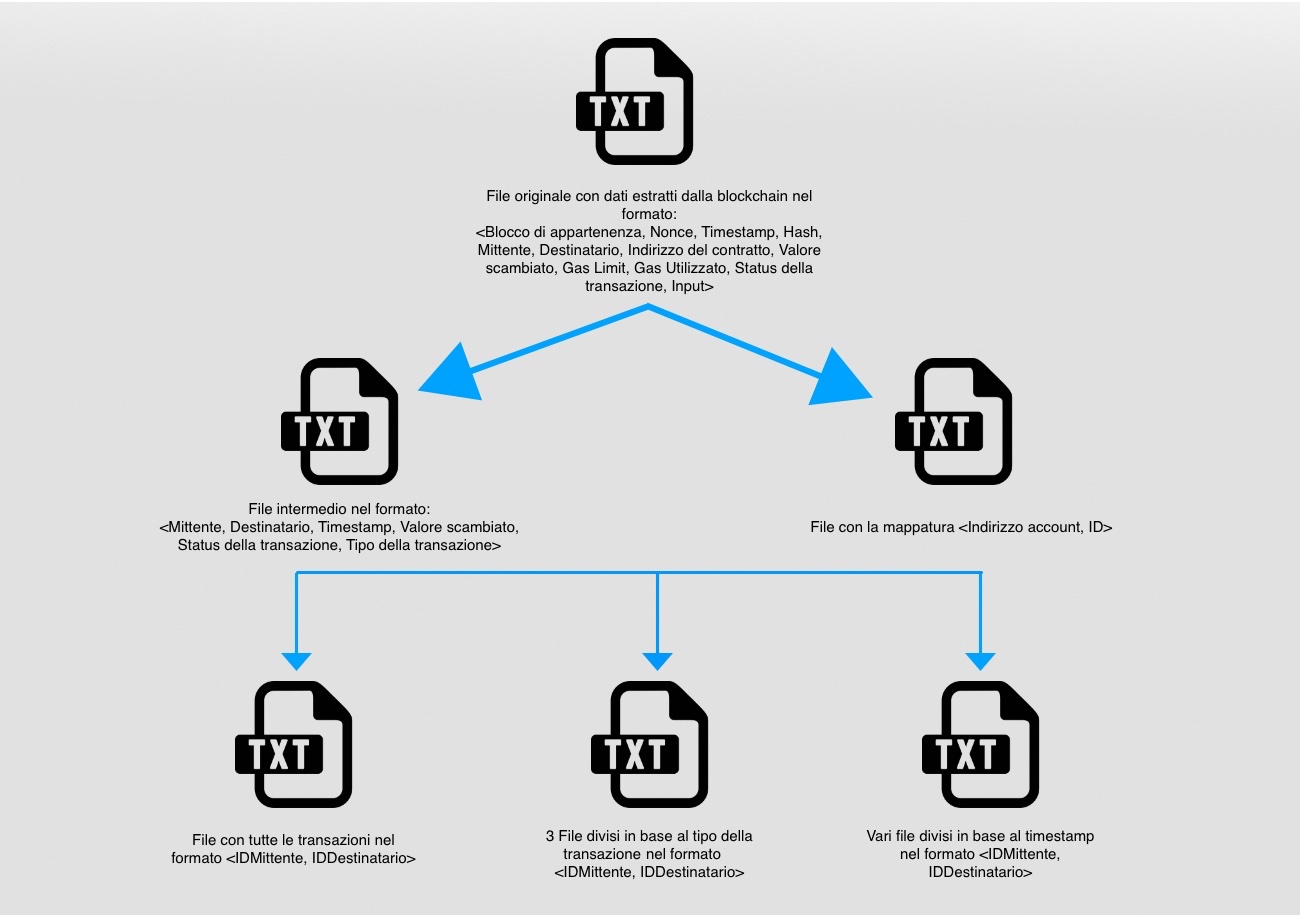
\includegraphics[width=\textwidth]{MappaFile}
    \caption{Organizzazione del dataset}
\end{figure}


Partendo dai file con le transazioni nel formato $<IDMittente, IDDestinatario>$ è stato poi possibile andare a produrre il grafo nel formato .webGraph.
Per questo ultimo passaggio è necessaria una ulteriore piccola modifica, è infatti possibile che tra due nodi della rete si sia verificata più di una transazione, per creare il nostro grafo ne abbiamo considerata esclusivamente una in modo da sapere solamente se i due nodi sono entrati in contatto o meno.
\newline Il file di testo da fornire a webgraph deve essere organizzato con il seguente formato:
\begin{itemize}
    \item Nella prima riga va indicato il numero totale di nodi del grafo;
    \item Ogni riga successiva rappresenta un nodo del grafo. Ad esempio, la seconda conterrà l'elenco dei nodi che sono connessi al primo nodo del grafo, la terza quelli connessi al secondo nodo e così via fino ad arrivare all'ultimo nodo.
    Nel file possiamo anche avere delle righe vuote, in questo caso vuol dire che quel nodo non ha archi uscenti ma ne avrà solamente alcuni entranti.
\end{itemize}
La creazione del grafo avviene da terminale, come si può vedere dall'immagine:

\begin{figure}[H]
    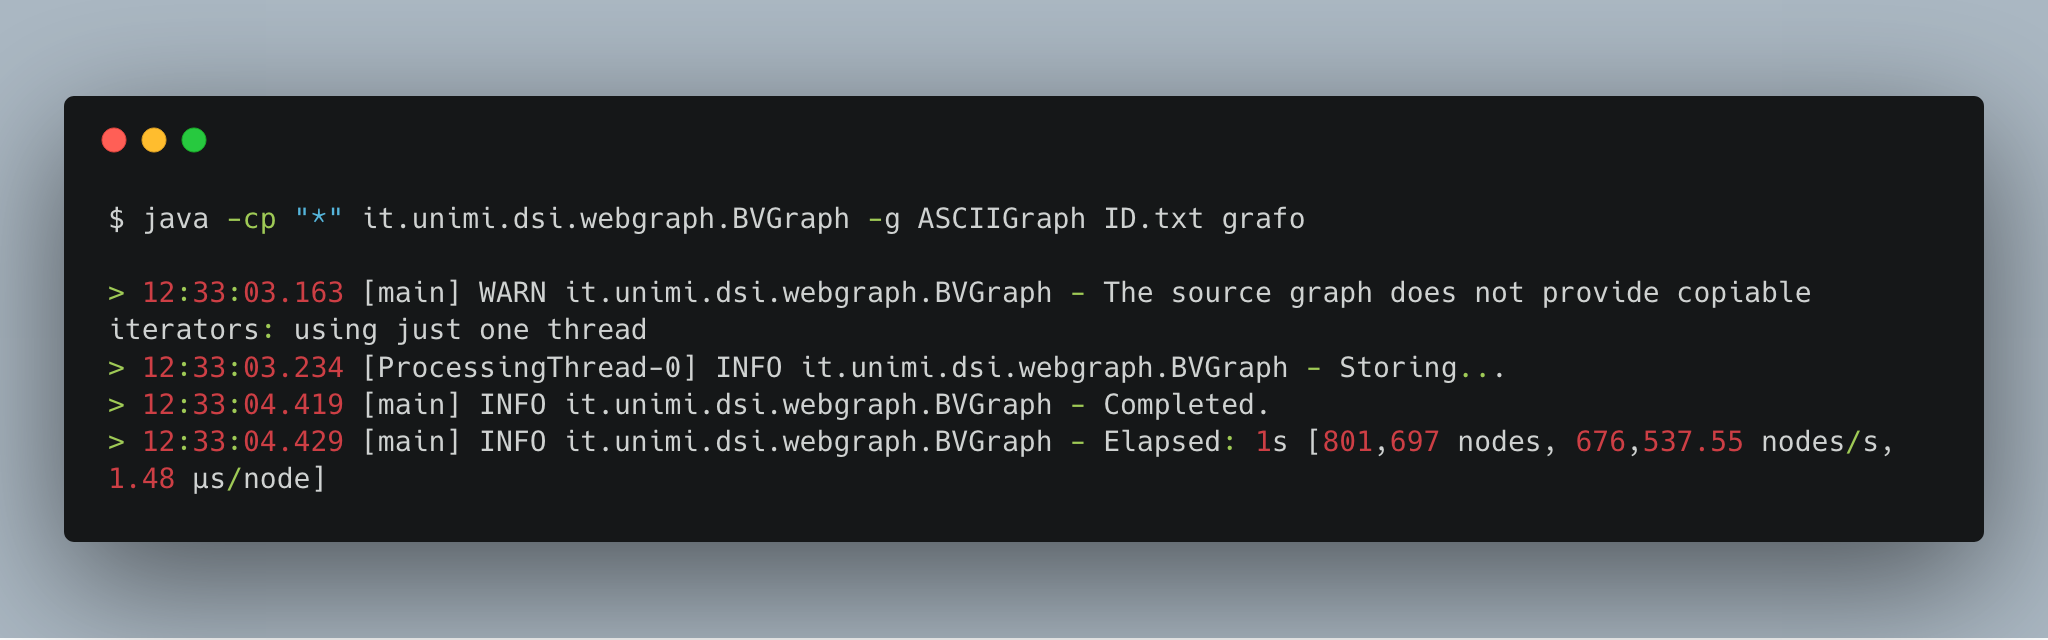
\includegraphics[width=\textwidth]{carbon-22.png}
    \caption{Creazione del grafo WebGraph}
\end{figure}

Questa procedura crea i seguenti file:

\begin{itemize}
    \item Grafo.graph, si tratta del file che rappresenta il grafo compresso;
    \item Grafo.offset;
    \item Grafo.properties, contiene alcuni dettagli riguardanti il grafo, come ad esempio il numero dei nodi.
\end{itemize}


Il grafo che è stato prodotto con i dati estratti dalla blockchain ci fornisce una rappresentazione delle transazioni che sono avvenute nel corso degli anni.

\begin{figure}[H]
    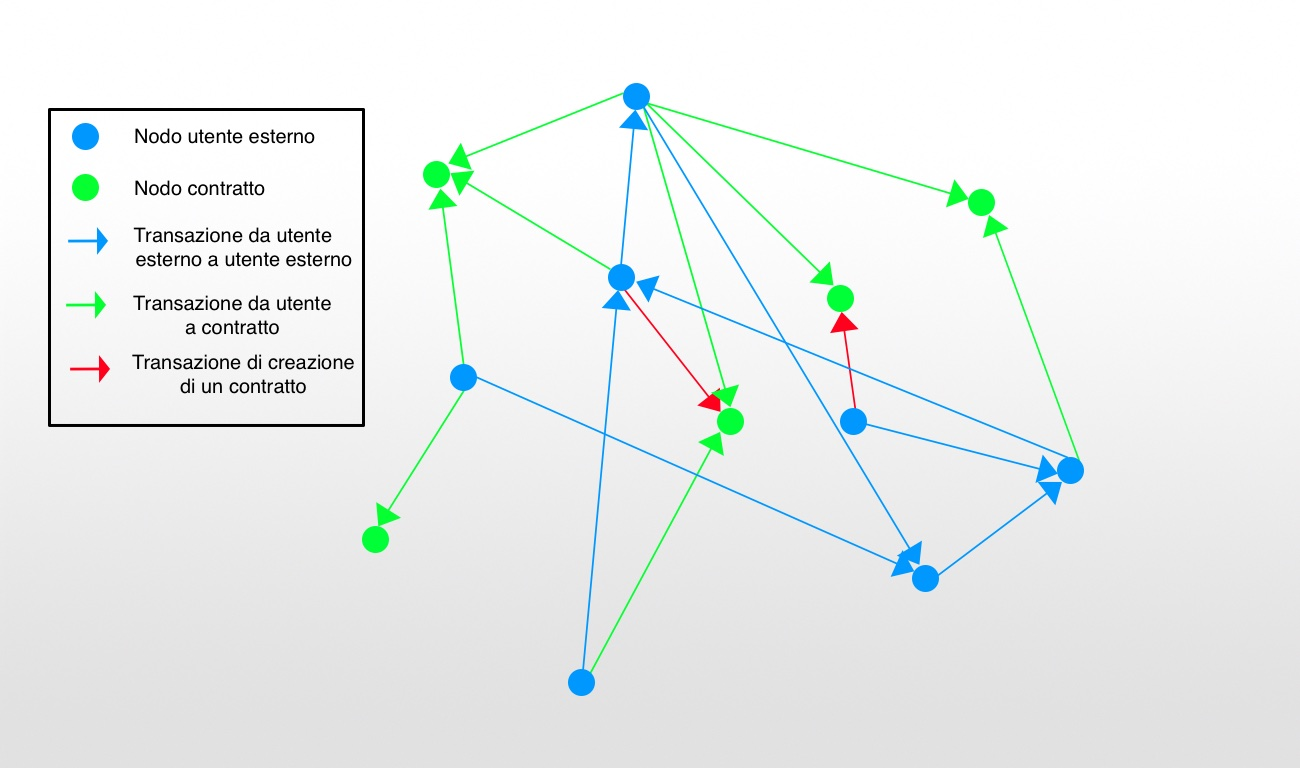
\includegraphics[width=\textwidth]{GrafoFinito.jpg}
    \caption{Rappresentazione grafica di una porzione di nodi e archi del grafo}
\end{figure}

Nel grafo i nodi rappresentano gli utenti della rete Ethereum, in particolare abbiamo:

\begin{itemize}
    \item Utenti esterni, colorati in blu nell'immagine;
    \item Contratti, di colore verde.
\end{itemize}

Gli archi nel grafo rappresentano invece le transazioni avvenute tra i vari nodi della rete, queste possono essere di tre tipi:

\begin{itemize}
    \item Transazioni da utente esterno ad utente esterno, di colore blu nella Figura 5.1;
    \item Transazioni da utente esterno a contratto, di colore verde nella Figura 5.1;
    \item Transazioni utilizzate per la creazione di un nuovo smart contract, in rosso nella Figura 5.1
\end{itemize}

\chapter{Risultati sperimentali}

L'obiettivo finale del tirocinio è quello di produrre un grafo che possa rappresentare le transazioni presenti nella blockchain di Ethereum. In questo capitolo descriviamo le analisi che sono state svolte con un notebook con processore Intel Quad-Core e 16 Gb di memoria Ram sui grafi creati con i dati estratti dalla blockchain.
\newline
Le analisi sono state svolte sia sul grafo completo sia su un insieme di snapshot temporali che ci hanno permesso di studiare l'evoluzione della rete Ethereum.
Infine sono state effettuate delle analisi anche sui grafi divisi in base al tipo delle transazioni.

\section{Analisi svolte sul grafo completo}

Le analisi svolte sul grafo completo riguardano le transazioni presenti nei blocchi compresi tra il numero 0 e il 4237648, queste coprono un periodo di tempo che va dal Luglio 2015 al Settembre 2017. Purtroppo non è stato possibile estrarre le informazioni dai blocchi successivi a causa dell'elevato costo computazionale dovuto all'aumento del numero delle transazioni di Ethereum nel corso dell'ultimo anno.
Il grafo che abbiamo creato partendo da questo insieme di transazioni comprende al suo interno 6081755 nodi e 7224840 archi.
L'analisi ci ha permesso di comprendere per prima cosa la distribuzione del grado uscente ed entrante dei nodi.
Queste due proprietà del grafo vengono mostrate nelle Figure 6.1 e 6.2.

\begin{figure}[H]
    \centering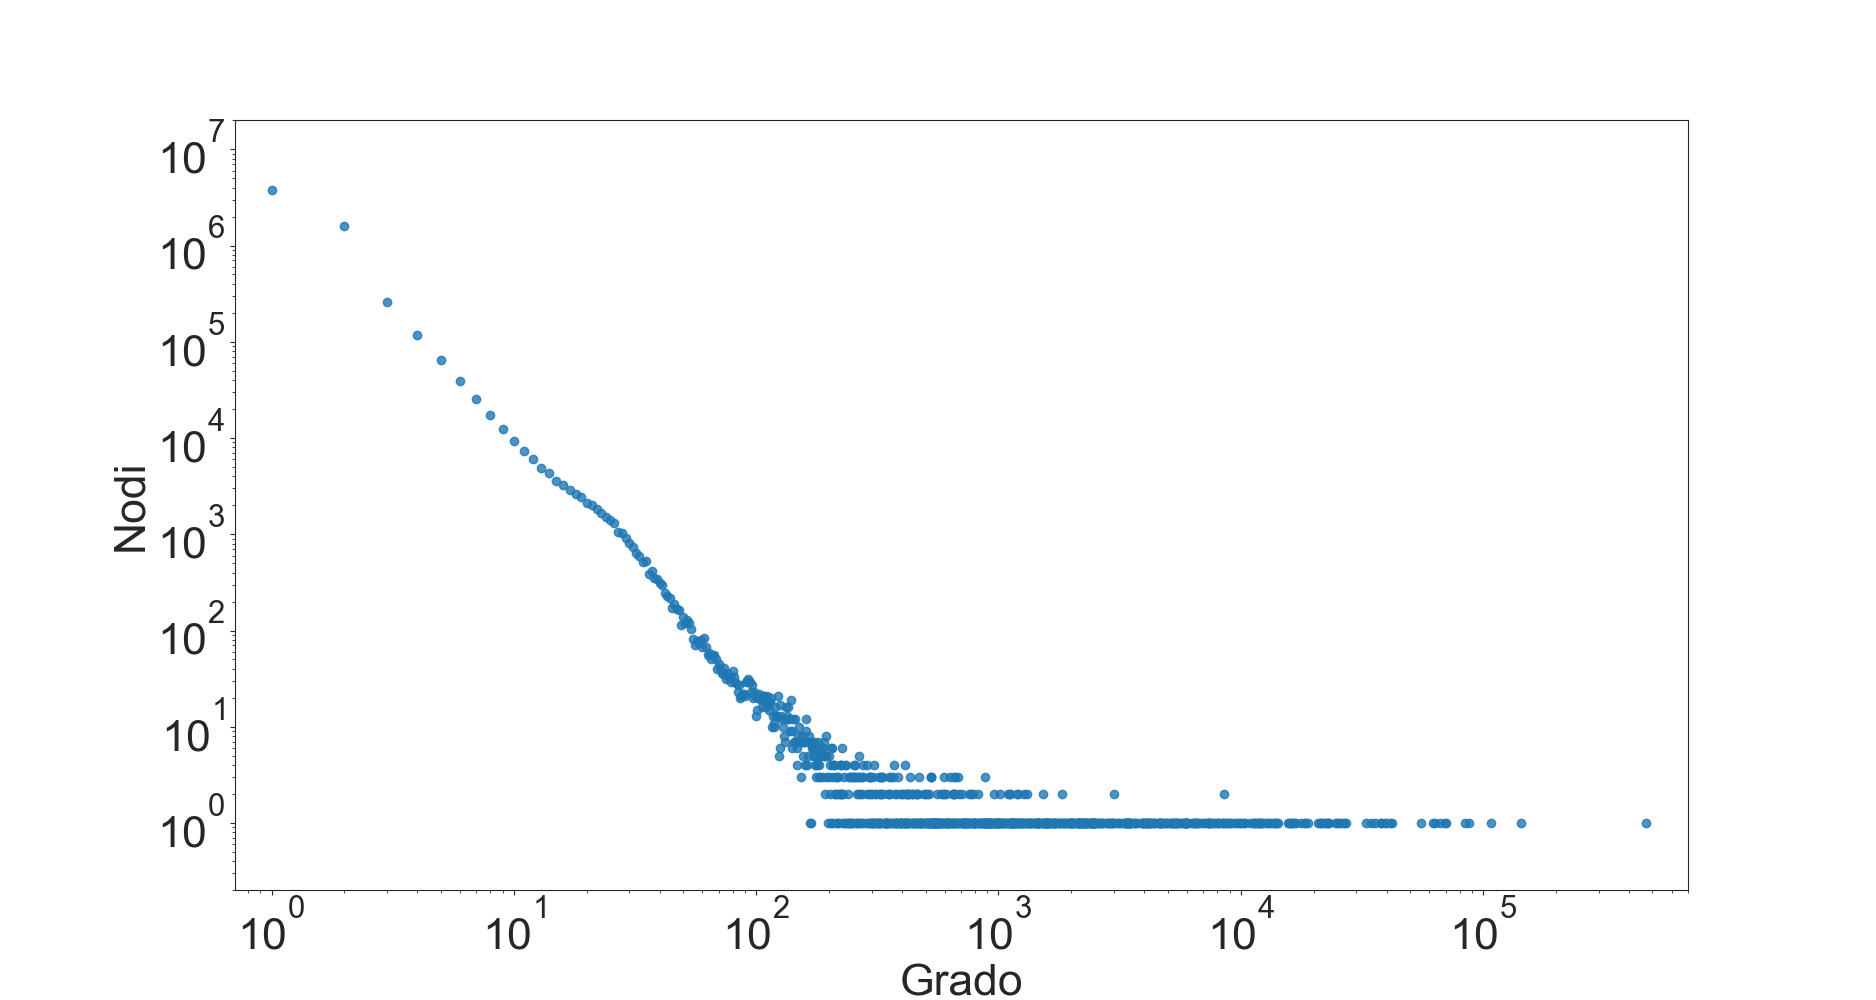
\includegraphics[width=\textwidth]{DirINDegreeDistribution.png}
        \caption{Distribuzione del grado entrante dei nodi nel grafo orientato}
\end{figure}
\begin{figure}[H]
        \centering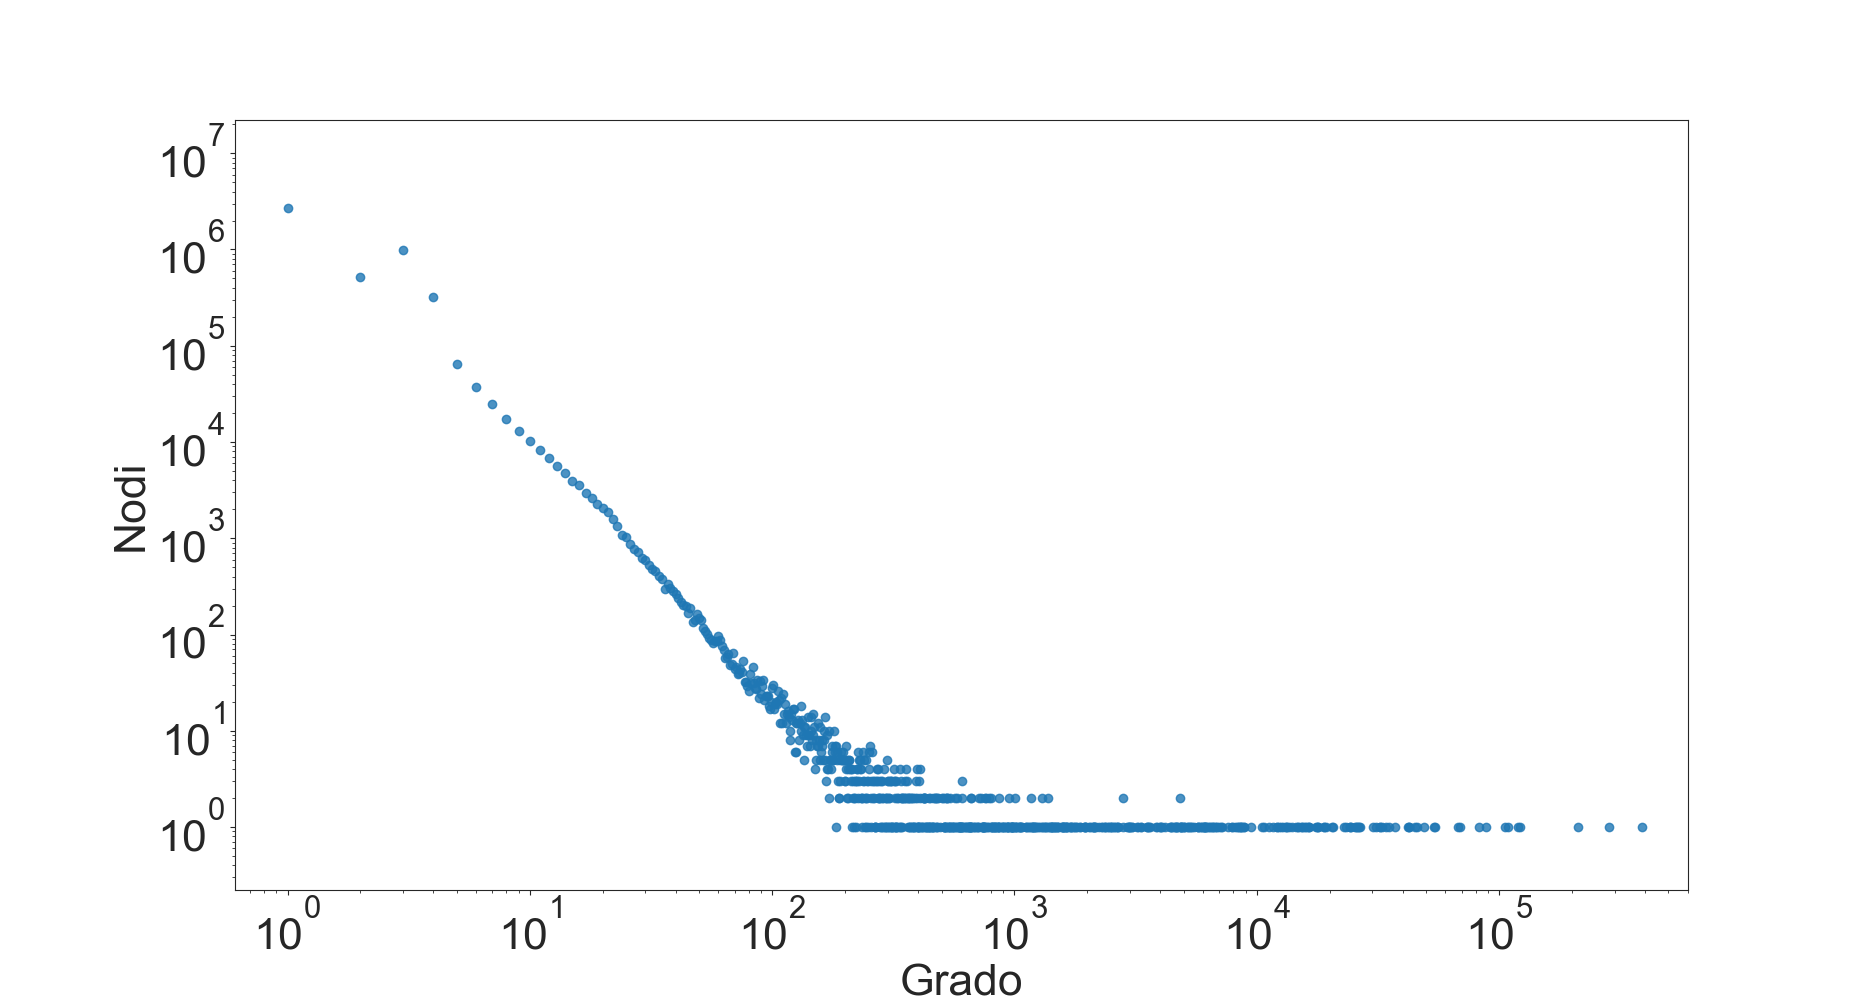
\includegraphics[width=\textwidth]{DirOUTDegreeDistribution.png}
        \caption{Distribuzione del grado uscente dei nodi nel grafo orientato}
\end{figure}
\newpage
Successivamente la stessa analisi è stata svolta anche sul grafo non orientato, in questo caso non facciamo differenza tra il grado entrante e quello uscente. Il risultato è mostrato nel grafico della Figura 6.3.

\begin{figure}[H]
    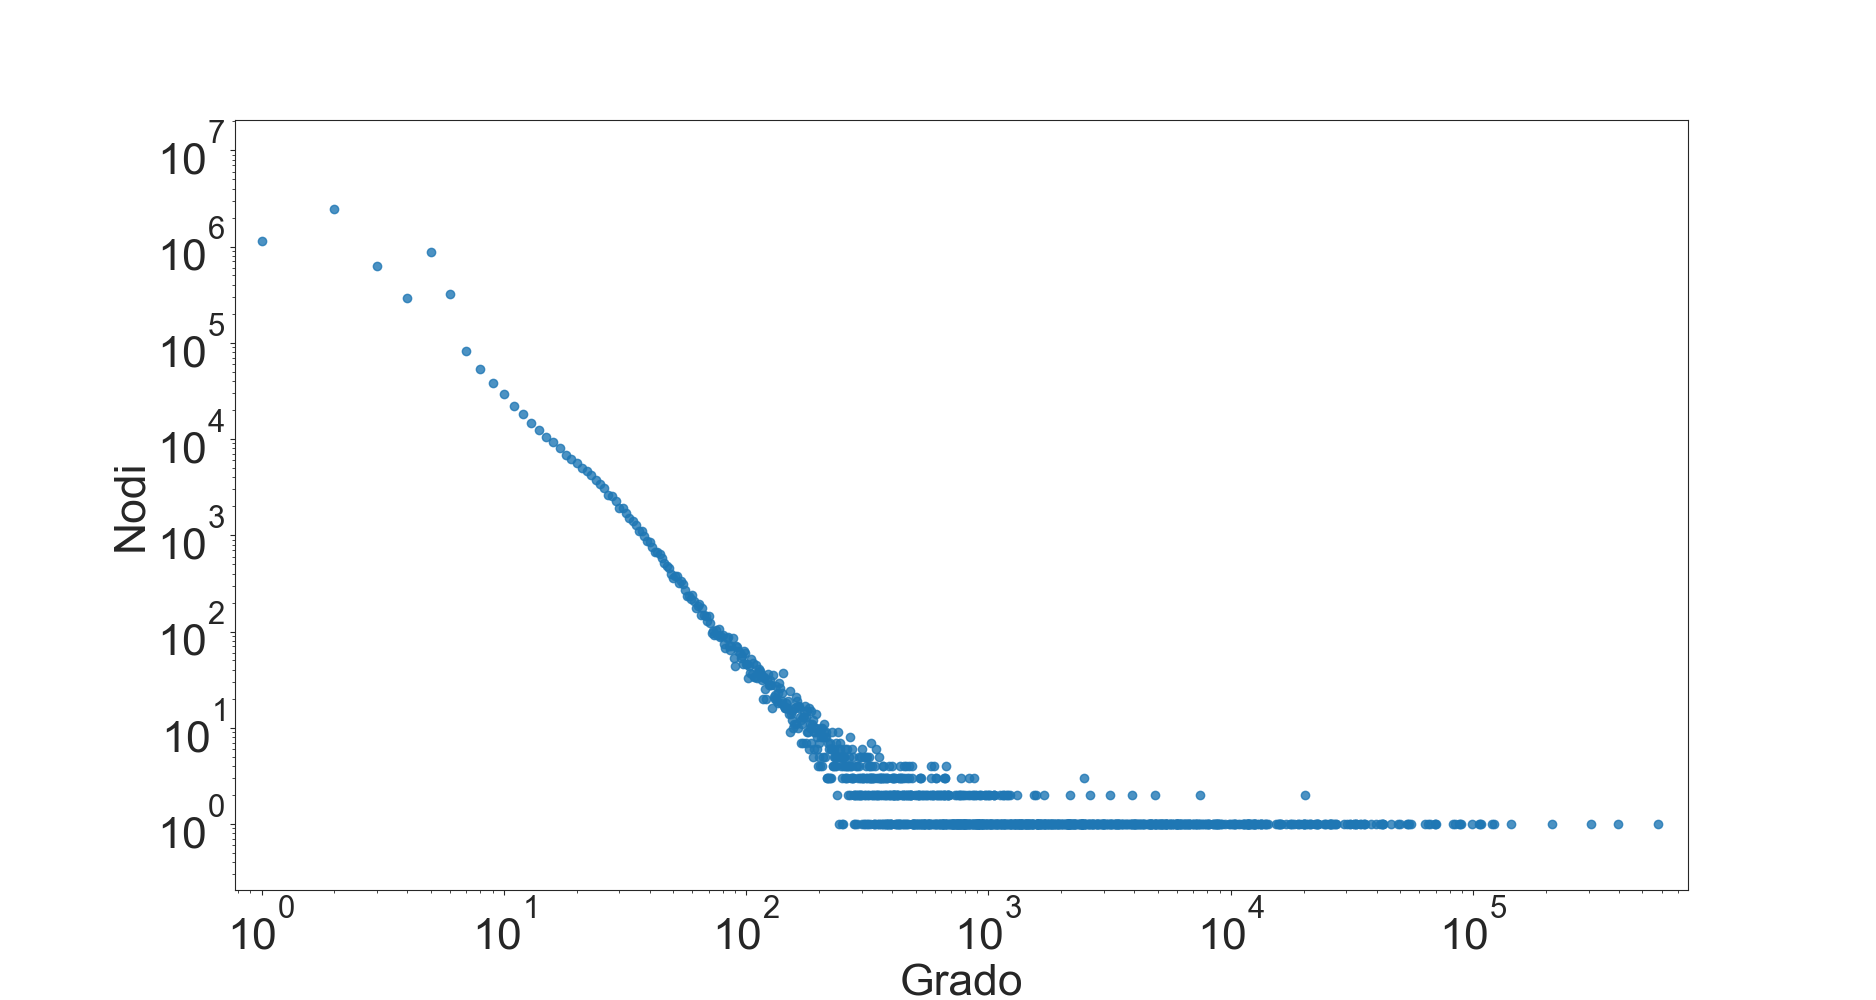
\includegraphics[width=\textwidth]{UndirDegreeDistribution.png}
    \caption{Distribuzione del grado dei nodi nel grafo non orientato}
\end{figure}

I grafici che mostrano le distribuzioni del grado sono rappresentati con la scala logaritmica che ci ha permesso di mostrare un maggior numero di dati all'interno del grafico.
\newline In tutti e tre i casi abbiamo avuto un comportamento di tipo power law e i risultati sono in linea con la proprietà small world.
Dalla Figura 6.1 osserviamo che molti nodi della rete hanno un grado entrante molto basso quindi ricevono poche transazioni. Allo stesso tempo ci sono pochi nodi che ricevono molte transazioni e hanno un alto grado entrante.
Le stesse osservazioni possono essere estese anche al grafico della Figura 6.2, in cui però consideriamo la quantità di transazioni inviate da ciascun utente e a quello della Figura 6.3 in cui non facciamo distinzione tra gli archi entranti e quelli uscenti.

Sul grafo completo è stata svolta anche l'analisi della distanza da cui è risultato che la distanza media tra i nodi è di 4.33863565559877 e il diametro 8267.
\newline
Il valore del diametro è risultato più alto del previsto, soprattutto se confrontato con la distanza media tra i nodi. Mentre quest'ultimo valore è in linea con la proprietà small world, il diametro non rispetta l'ipotesi secondo la quale la lunghezza dovrebbe essere logaritmica rispetto al numero di nodi del grafo.

Basandoci sugli studi già svolti sul grafo di Bitcoin \cite{maesa2017detecting} abbiamo quindi ipotizzato che la catena di transazioni che troviamo nel percorso del diametro sia dovuta ad un lungo cammino artificiale.
\newline
È stata studiata anche la distribuzione delle distanze tra i nodi che viene mostrata nel grafico 6.4, in questo caso sull'asse delle ascisse troviamo la distanza tra i nodi mentre sull'asse delle ordinate la percentuale di coppie di nodi che si trovano a quella determinata distanza.
In questo caso la scala logaritmica è stata utilizzata solamente sull'asse delle ascisse. 
Questa scelta è dovuta al fatto che, utilizzando la scala logaritmica anche sull'asse delle ordinate, sarebbero state mostrate delle spike dovute ad errori del metodo implementato in WebGraph per il calcolo della distribuzione delle distanze.
Prima di passare dalla rappresentazione con entrambi gli assi in scala logaritmica a quella della Figura 6.4 abbiamo effettuato vari test su set di nodi selezionati casualmente dal dataset completo. 
Questo ci ha consentito di essere sicuri che le spike fossero effettivamente dovute ad errori del metodo.
Il risultato di questa analisi mostra, per valori bassi della distanza, una forma a ``campana`` del grafico. La maggior parte delle coppie di nodi si trovano ad una distanza compresa tra 1 e 10, questo dato viene anche confermato dal valore della distanza media tra i nodi. 
Con l'aumentare del valore $d$ della distanza, scende la percentuale delle coppie di nodi che si trovano a distanza $d$.

\begin{figure}[H]
    \centering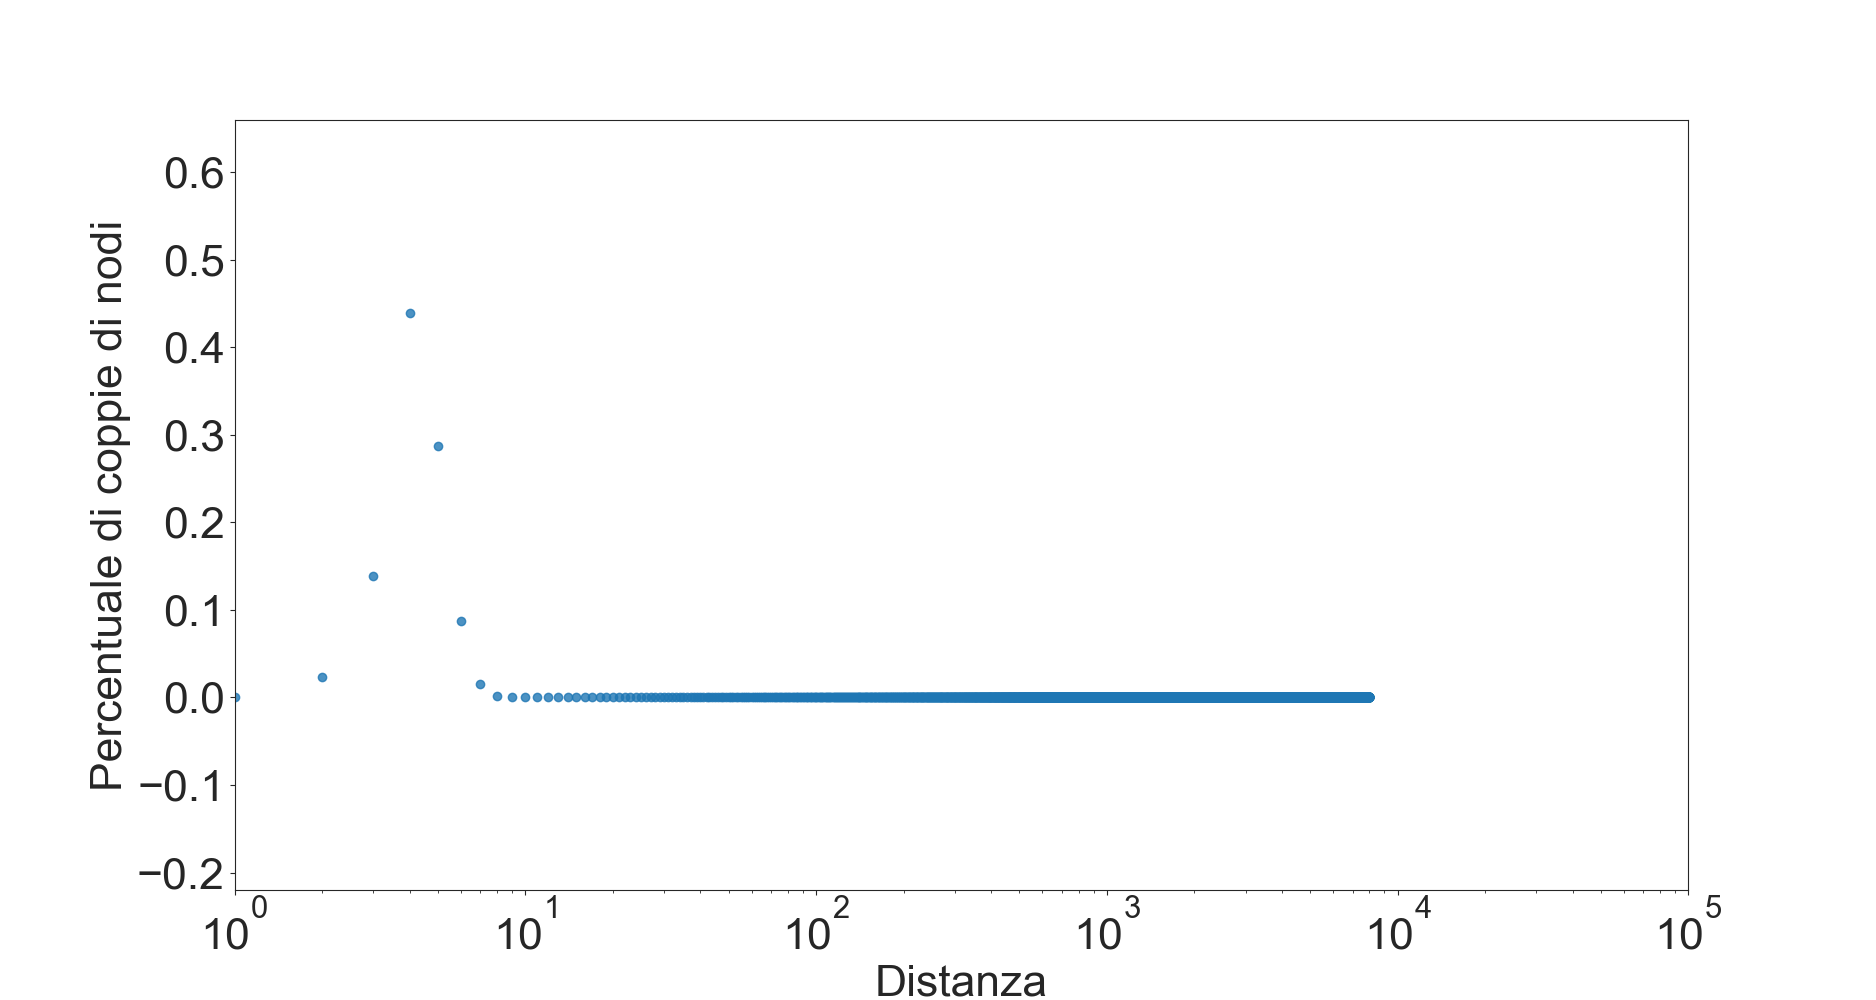
\includegraphics[width=0.8\textwidth]{DistribuzioneLogX.png}
    \caption{Distribuzione delle distanze tra i nodi}
\end{figure}

L'analisi più costosa, in termini di potenza computazionale richiesta, è stata quella relativa alle centralità del grafo. Come già indicato prima, esistono diverse misure di centralità.
Avendo già a disposizione i dati riguardanti il grado dei nodi, ci siamo basati su questa misurazione per generare una prima lista di account particolarmente attivi nella rete.
Il software di analisi ci ha restituito una lista di ID, successivamente abbiamo cercato, nei limiti del possibile, di associare questi ID ad un nome utilizzando Etherscan \cite{Etherscan}.

\begin{table}[H]
\centering
\begin{tabular}{ |c|c|c| } 
\hline
Indirizzo & Archi entranti & Nome \\
\hline
\multirow
0xfbb1b73c4f0bda4f67dca266ce6ef42f520fbb98 & 390346 & Bittrex_1\\ 
0x32be343b94f860124dc4fee278fdcbd38c102d88 & 285307 & Poloniex_1\\ 
0xb42b20ddbeabdc2a288be7ff847ff94fb48d2579 & 210984 &  \\ 
0xea674fdde714fd979de3edf0f56aa9716b898ec8 & 122359 & Ethermine\\ 
0x267be1c1d684f78cb4f6a176c4911b741e4ffdc0 & 119312 & Kraken_4\\ 
0x70faa28a6b8d6829a4b1e649d26ec9a2a39ba413 & 108719 & ShapeShift\\ 
0x42da8a05cb7ed9a43572b5ba1b8f82a0a6e263dc & 105605 & Yunbi_2\\ 
0x52bc44d5378309ee2abf1539bf71de1b7d7be3b5 & 88463 & Nanopool\\ 
0xd94c9ff168dc6aebf9b6cc86deff54f3fb0afc33 & 82843 & Yunbi_1\\ 
0x7ed1e469fcb3ee19c0366d829e291451be638e59 & 69055 & Freewallet\\
\hline 
\end{tabular}
\caption{Top 10 account per archi numero di archi entranti}
\end{table}


\begin{table}[H]

\centering

\begin{tabular}{ |c|c|c| } 
\hline
Indirizzo & Archi uscenti & Nome\\
\hline
\multirow
0x70faa28a6b8d6829a4b1e649d26ec9a2a39ba413 & 468932 & ShapeShift\\ 
0xe94b04a0fed112f3664e45adb2b8915693dd5ff3 & 143739 & Bittrex_2\\ 
0xfa52274dd61e1643d2205169732f29114bc240b3 & 107762 & Kraken_5\\ 
0x209c4784ab1e8183cf58ca33cb740efbf3fc18ef & 87302 & Poloniex_3\\ 
0x86fa049857e0209aa7d9e616f7eb3b3b78ecfdb0 & 84275 & EOSTokenContract\\ 
0xa74476443119a942de498590fe1f2454d7d4ac0d & 70278 & Golem\\ 
0x7727e5113d1d161373623e5f49fd568b4f543a9e & 69511 & Bitfinex_2\\ 
0xaa1a6e3e6ef20068f7f8d8c835d2d22fd5116444 & 66500 & ReplaySafeSplit\\ 
0x0064454b14cddc990ed6520ef94d3e28fe7c41b6 & 63114 & \\ 
0x96fc4553a00c117c5b0bed950dd625d1c16dc894 & 62028 & Changelly\\
\hline 
\end{tabular}
\caption{Top 10 account per archi numero di archi uscenti}
\end{table}

Abbiamo anche calcolato la centralità armonica nel grafo orientato.
Anche in questo caso abbiamo cercato, ove possibile, di associare all'indirizzo dell'account anche un nome.
Per calcolare questa misura di centralità è stata necessaria un'analisi che ha richiesto più di 50 ore.

\begin{table}[H]
\centering
\begin{tabular}{ |c|c|c|c| } 
\hline
Indirizzo & Centralità Armonica & Nome \\
\hline
\multirow

0x32be343b94f860124dc4fee278fdcbd38c102d88 & 2037051.1 & Poloniex_1\\
0xfbb1b73c4f0bda4f67dca266ce6ef42f520fbb98 & 1967112.5 & Bittrex_1 \\
0x7ed1e469fcb3ee19c0366d829e291451be638e59 & 1764614.1 & Freewallet\\
0x267be1c1d684f78cb4f6a176c4911b741e4ffdc0 & 1729339.6 & Kraken_4\\
0x70faa28a6b8d6829a4b1e649d26ec9a2a39ba413 & 1725644.1 & ShapeShift \\
0x1151314c646ce4e0efd76d1af4760ae66a9fe30f & 1671783.1 & Bitfinex_1\\
0x563b377a956c80d77a7c613a9343699ad6123911 & 1611149.1 & \\
0xea674fdde714fd979de3edf0f56aa9716b898ec8 & 1590653.1 & Ethermine\\
0x2a65aca4d5fc5b5c859090a6c34d164135398226 & 1590188.2 & DwarfPool_1\\
0x22b84d5ffea8b801c0422afe752377a64aa738c2 & 1580784.5 & \\
\hline 
\end{tabular}
\caption{Top 10 nodi per Centralità Armonica}
\end{table}

Confrontando le Tabelle 6.2 e 6.3 notiamo che alcuni dei nodi risultano essere centrali con entrambe le misurazioni, stiamo parlando in particolare di indirizzi riconducibili a vari exchange come Bittrex, Kraken, Poloniex, ShapeShift.
Nella sezione 6.2 verranno analizzati più nel dettaglio questi nodi cercando di comprendere il motivo per cui sono i più centrali nella rete.



\newpage
\section{Analisi svolte sugli snapshot}

Nella seconda fase dell'analisi, abbiamo studiato l'evoluzione nel corso del tempo del grafo delle transazioni $G$.
Grazie al timestamp presente all'interno di ogni blocco, è stato possibile suddividere l'insieme delle transazioni in periodi temporali equidistanti e di lunghezza fissata in modo da studiare l'evoluzione nel tempo della rete Ethereum.
\newline 
Siamo partiti con le transazioni del blocco 0 del Luglio 2015 e siamo arrivati al 4227609 del 1 Settembre 2017.
Per valori crescenti di T sono stati considerati dei grafi $G^T$ contenenti tutte le transazioni inviate nella rete al tempo T' con $T' \le T$.
La seguente tabella mostra la divisione effettuata:

\begin{table}[H]
\centering
\begin{tabular}{ |c|c|c|c| } 
\hline
Blocco & Timestamp & Data & Id Snapshot \\
\hline
\multirow
263500 & 1442763412 & 20 Settembre 2015 & 0\\ 
486745 & 1446608625 & 4 Novembre 2015 & 1\\ 
711283 & 1450453907 & 18 Dicembre 2015 & 2\\ 
935478 & 1454299094 & 1 Febbraio 2016 & 3\\ 
1161134 & 1458144274 & 16 Marzo 2016 & 4\\ 
1429370 & 1461989510 & 30 Aprile 2016 & 5\\ 
1697544 & 1465834685 & 13 Giugno 2016 & 6\\ 
1965769 & 1469679869 & 28 Luglio 2016 & 7\\ 
2234642 & 1473525063 & 10 Settembre 2016 & 8\\
2503209 & 1477370237 & 25 Ottobre 2016 & 9\\
2771418 & 1481215413 & 8 Dicembre 2016 & 10\\
3041034 & 1485060622 & 22 Gennaio 2017 & 11\\
3309427 & 1488905801 & 7 Marzo 2017 & 12\\
3572913 & 1492750975 & 21 Aprile 2017 & 13\\
3820049 & 1496596188 & 4 Giugno 2017 & 14\\
4042446 & 1500441393 & 19 Luglio 2017 & 15\\
4227609 & 1504243381 & 1 Settembre 2017 & 16\\
\hline 
\end{tabular}
\caption{Divisione del dataset in snapshot temporali}
\end{table}

\newpage
La prima analisi effettuata su questi snapshot temporali è stata quella riguardante il numero di nodi nella rete e le transazioni effettuate.
I risultati sono mostrati nelle Figure 6.5 e 6.6.
In particolare possiamo notare tra lo snapshot 0 e il 12 una crescita abbastanza regolare del numero di nodi e archi. 
A partire dallo snapshot 13 e soprattutto nel 15 e nel 16, corrispondenti al periodo compreso tra Giugno e Settembre 2017, abbiamo invece un aumento decisamente più rapido che porta il numero di nodi ad oltre 6 milioni.

\begin{figure}[H]
\centering
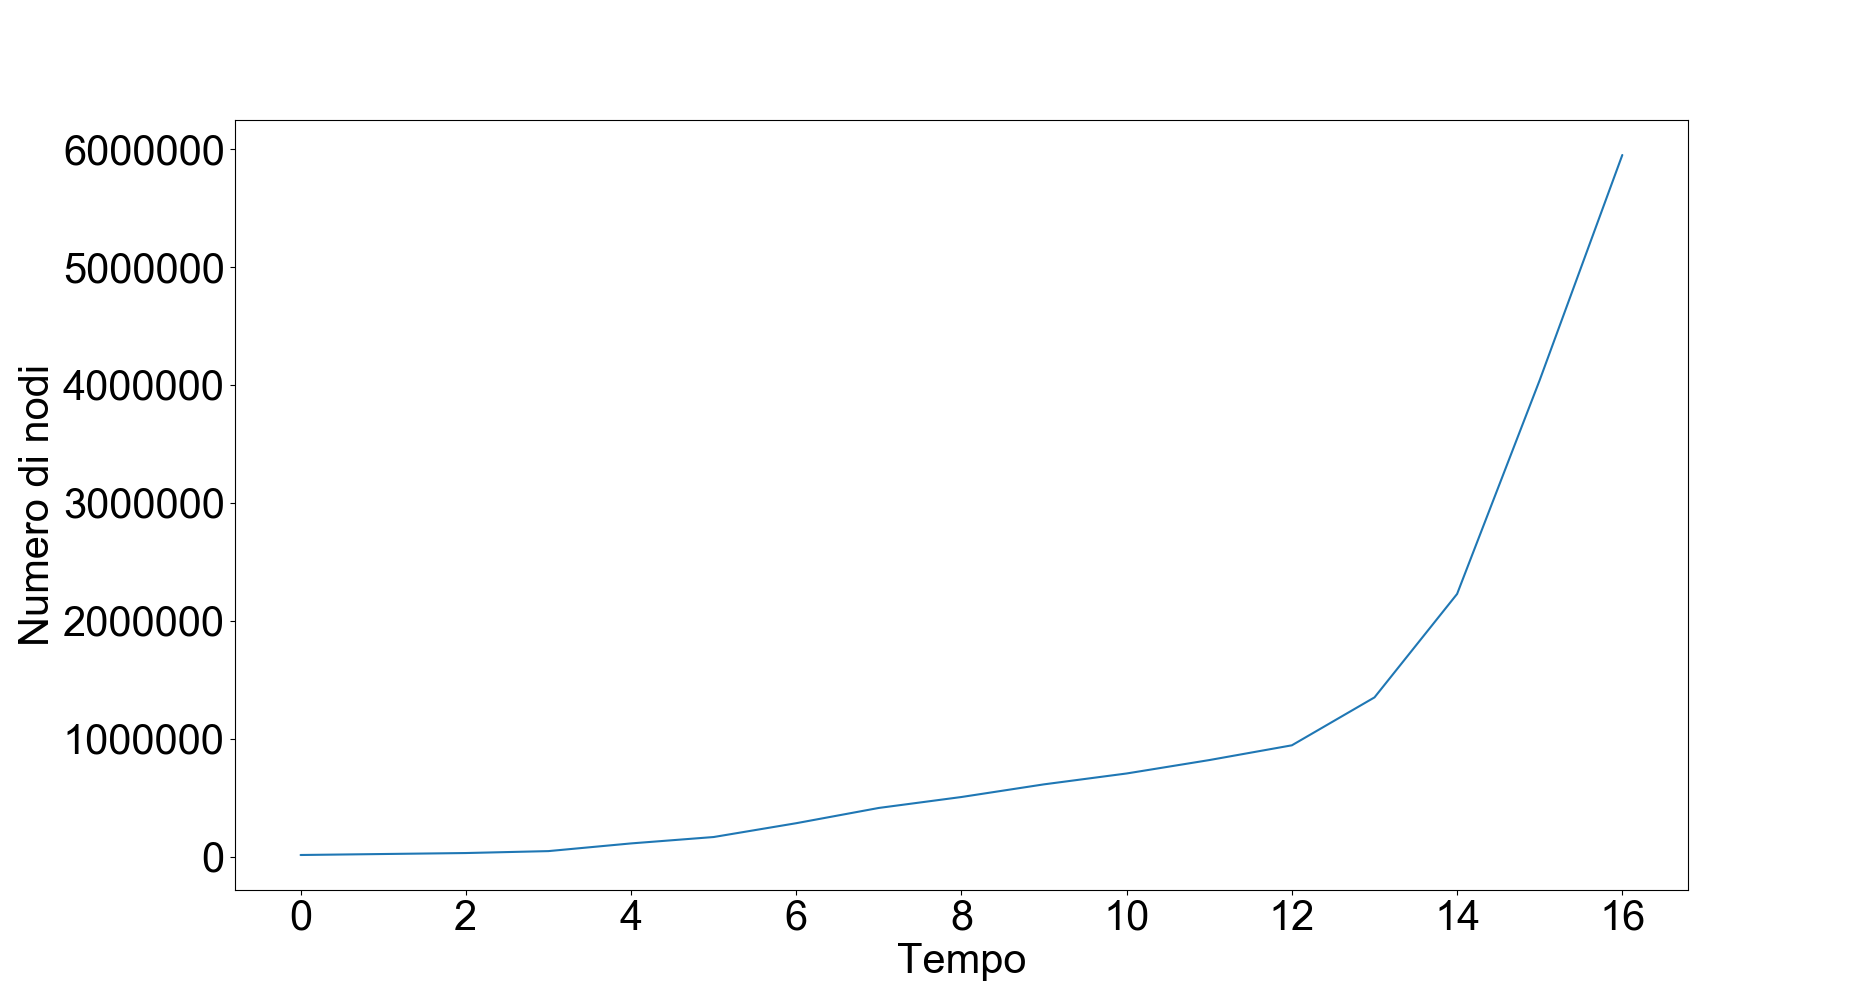
\includegraphics[width=0.9\textwidth]{PlotNumNodi.png}
\caption{Crescita del numero di nodi}
\end{figure}

\begin{figure}[H]
\centering  
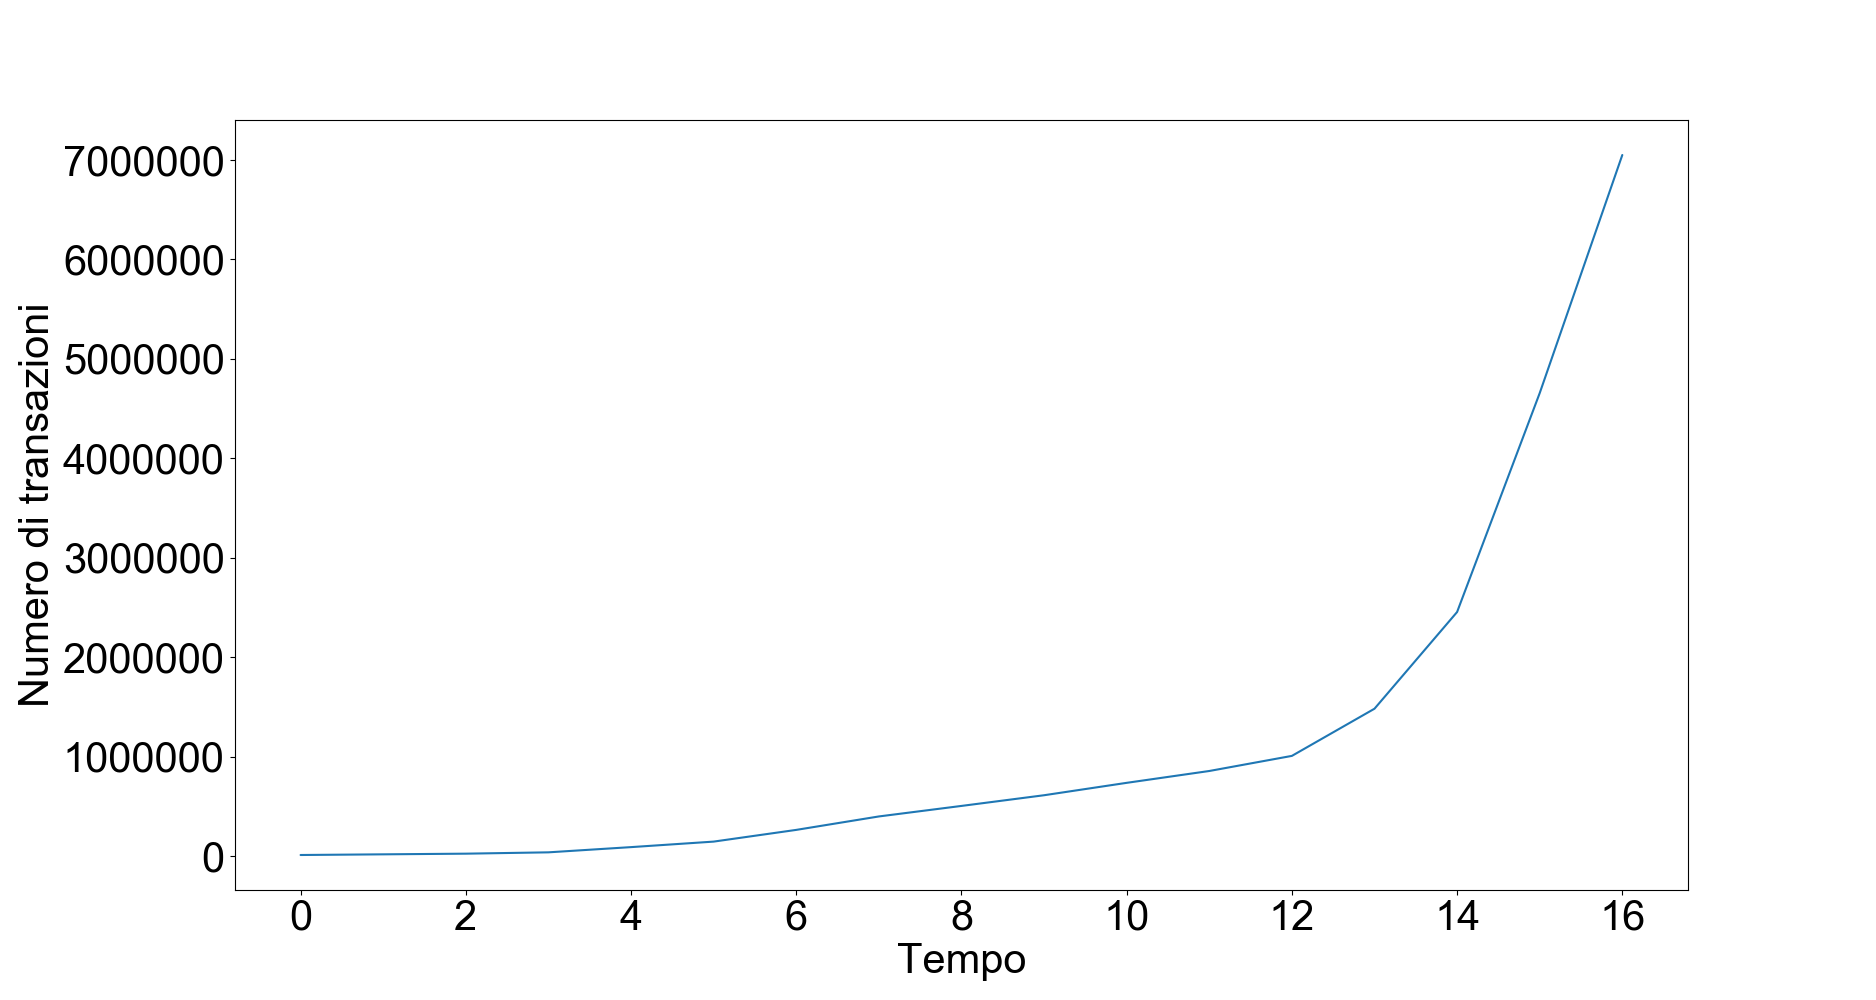
\includegraphics[width=0.9\textwidth]{PlotArchi.png}
\caption{Crescita del numero delle transazioni}
\end{figure}

Questo aumento improvviso di nodi nella rete è probabilmente legato alla crescita del valore di Ethereum che si è verificata nel periodo compreso tra Maggio e Settembre 2017. In questo periodo infatti il valore dell'Ether è passato da circa 80\$ a più di 300\$ come mostriamo nella Figura 6.7. Per lo stesso motivo è aumentato, nello stesso periodo, anche il numero delle transazioni.

\begin{figure}[H]
\centering  
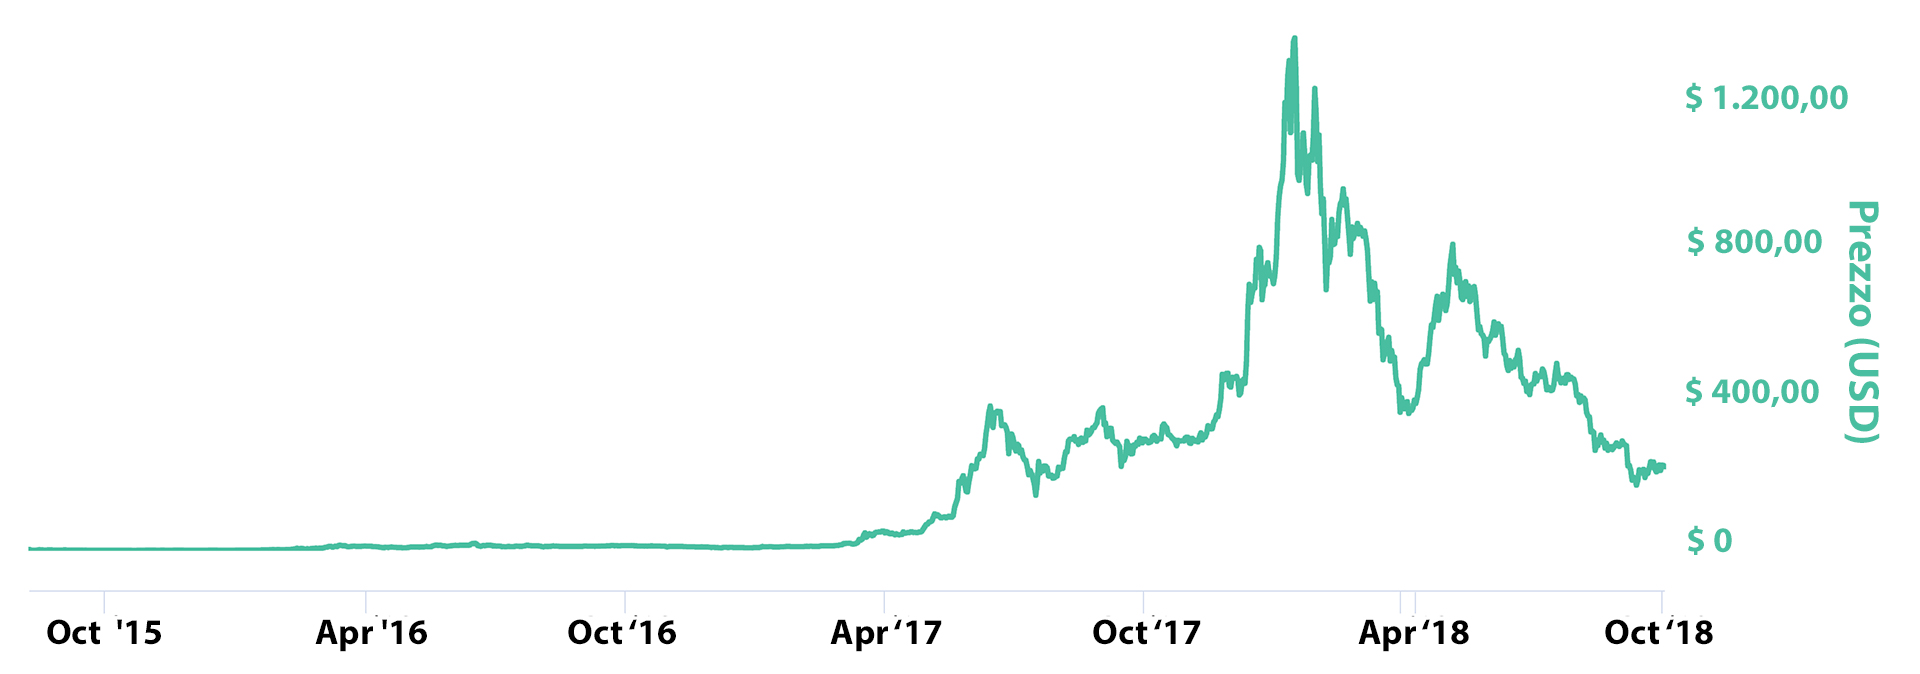
\includegraphics[width=\textwidth]{chart-2.jpg}
\caption{Variazione del valore dell'Ether}
\end{figure}


Abbiamo anche voluto mettere a confronto i grafici delle Figure 6.5 e 6.6 sovrapponendoli e ne è risultato che la crescita del numero dei nodi segue lo stesso andamento del numero delle transazioni, come mostrato nel grafico della Figura 6.8.

\begin{figure}[H]
    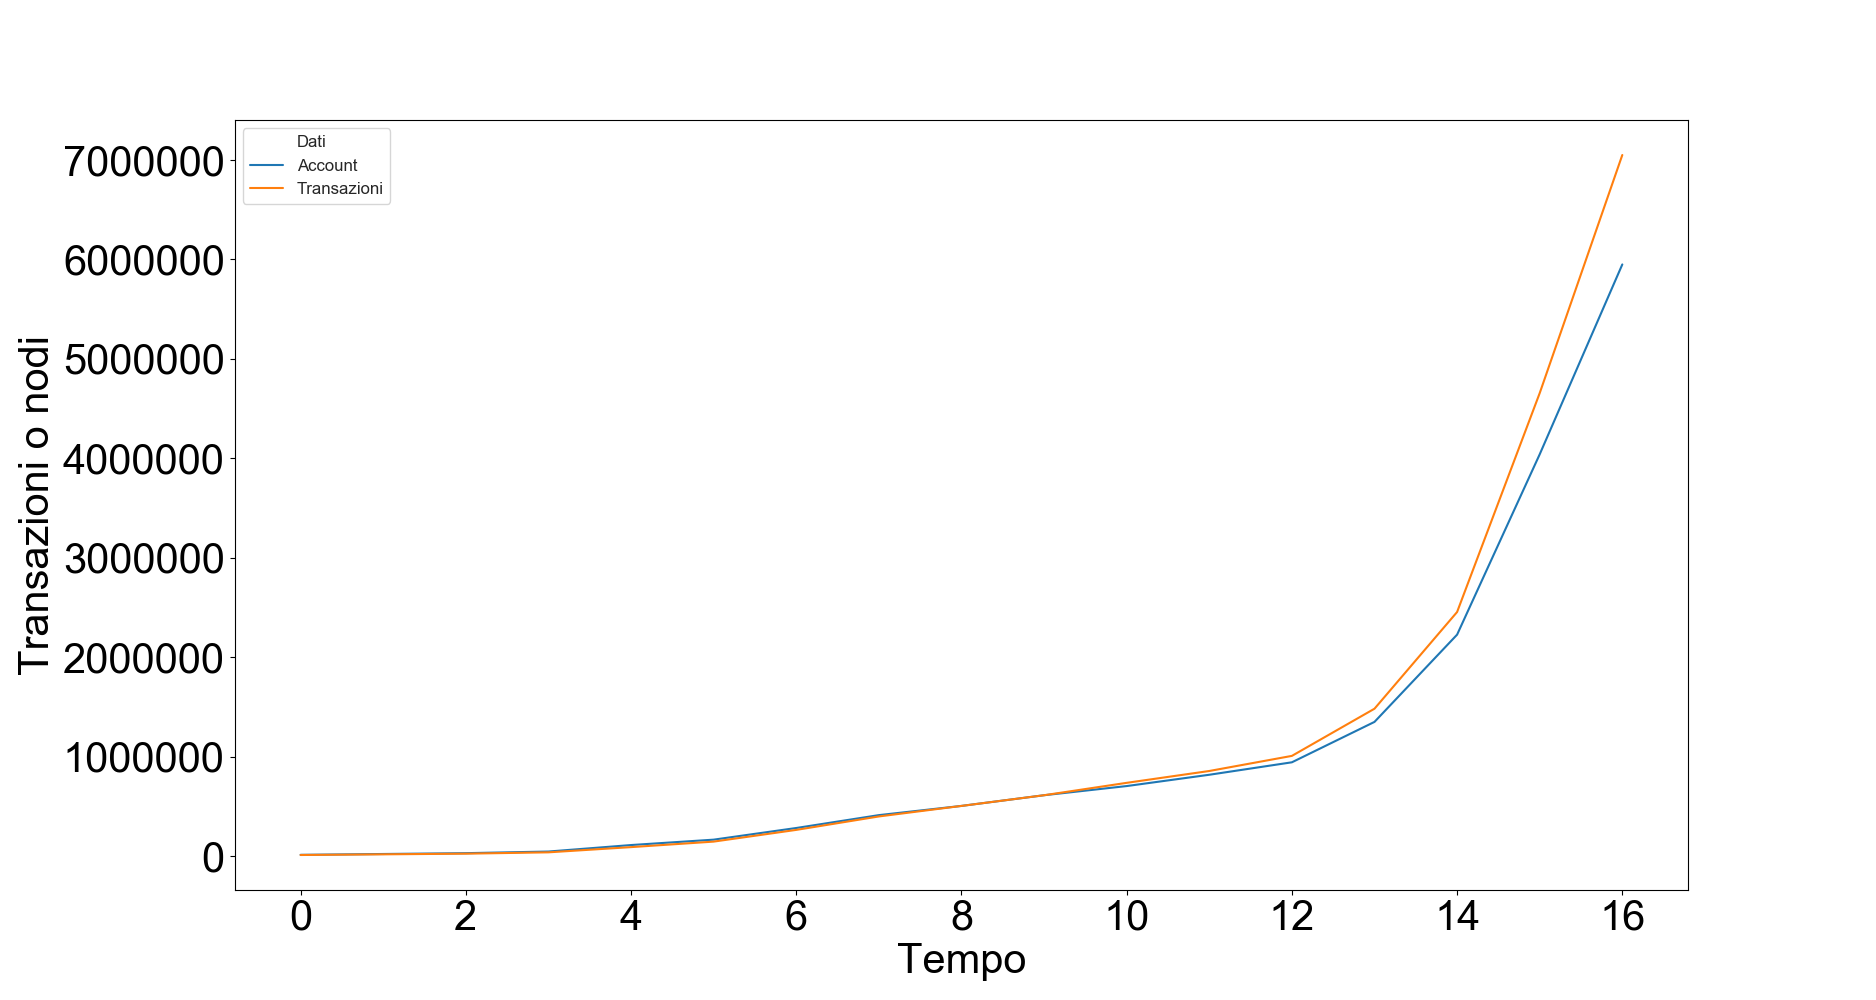
\includegraphics[width=\textwidth]{NodiETransazioni.png}
    \caption{Crescita dei nodi e delle transazioni a confronto}
\end{figure}

Il valore del grado dei nodi è invece cresciuto tantissimo con il passare del tempo. 
In particolare nella figura 6.9 evidenziamo il grado medio dei nodi nel grafo orientato e nella 6.10 il grado nel grafo non orientato.
Nella Figura 6.9 possiamo vedere come il grado medio dei nodi nel grafo orientato scenda sotto 1.7 nello snapshot 4 e poi inizi una crescita fino all'ultimo snapshot.
Anche nella figura 6.10, possiamo notare la medesima diminuzione del valore del grafo in corrispondenza dello snapshot 4.


\begin{figure}[H]

\centering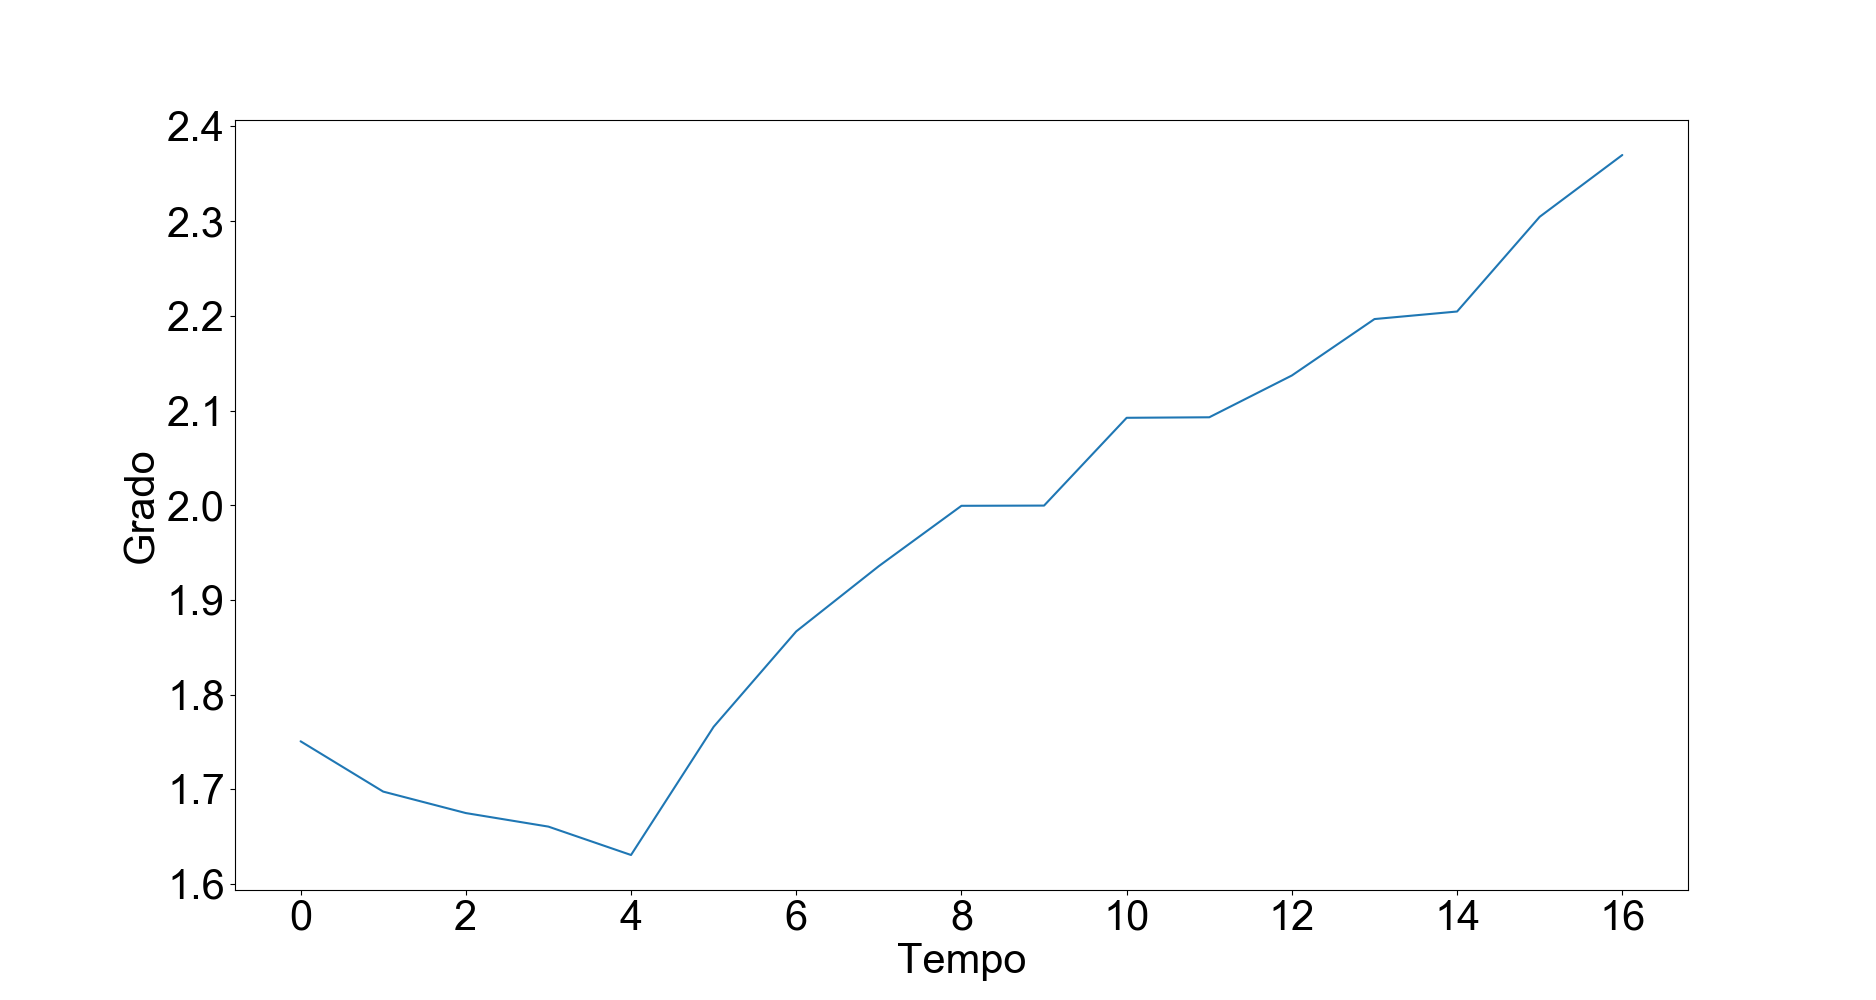
\includegraphics[width=0.9\textwidth]{GradoMedio.png}
\caption{Grado medio uscente dei nodi nel grafo orientato}

\end{figure}


\begin{figure}[H]

\centering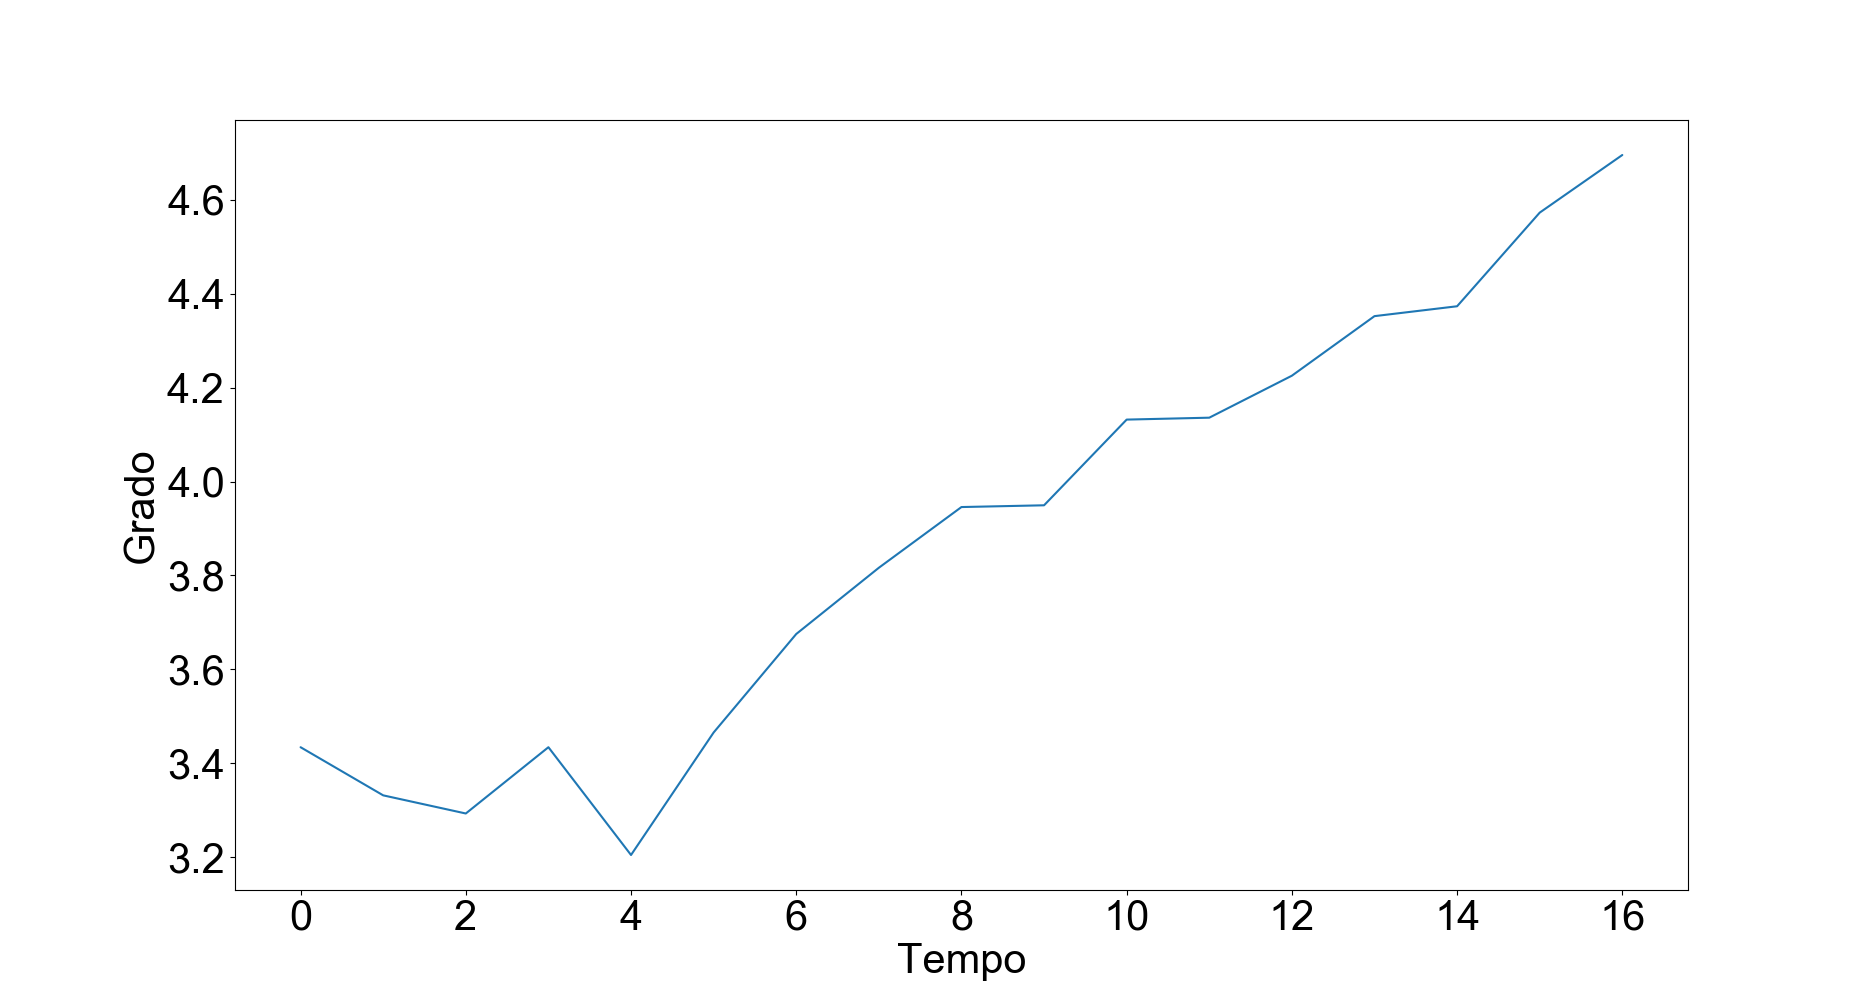
\includegraphics[width=0.9\textwidth]{GradoMedioUndir.png}
\caption{Grado medio dei nodi nel grafo non orientato}

\end{figure}


L'analisi delle distanze sui vari snapshot ci ha permesso di studiare l'evoluzione del diametro del grafo. Partendo da una lunghezza pari a 16, il diametro cresce fino ad avere lunghezza 8268 nel quarto snapshot. 
Da segnalare un minimo toccato nello snapshot 6 dove il diametro del grafo ha una lunghezza pari a 5003. Questa diminuzione del diametro del grafo potrebbe essere dovuta ad un nodo che ha fatto da ponte andando a rendere più breve il cammino del diametro stesso.
Dopo il minimo il diametro è tornato al valore 8267, valore mantenuto costante fino all'ultimo snapshot.
Come già indicato nella sezione 6.1, il valore del diametro è stato probabilmente influenzato da una serie di cammini artificiali anomali. Grazie all'analisi sugli snapshot possiamo notare che l'introduzione di questi cammini è avvenuta tra il periodo 3 ed il 4. 

\begin{figure}[H]
    \centering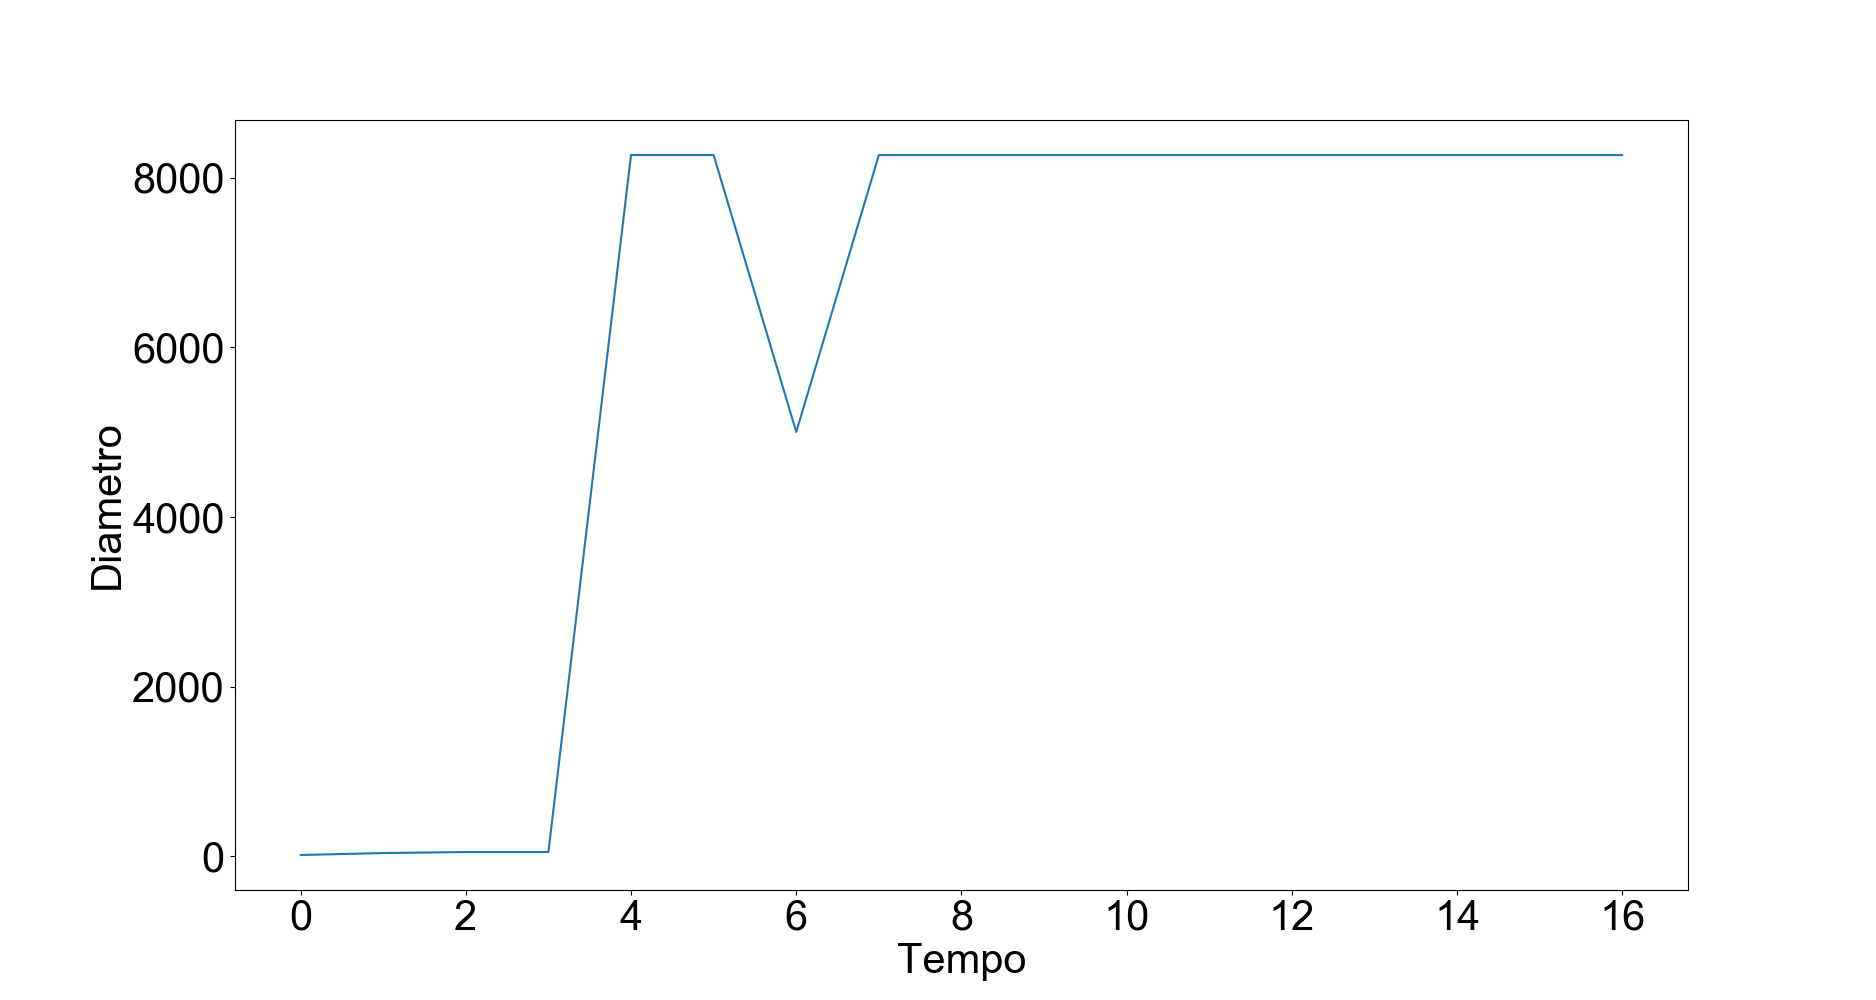
\includegraphics[width=0.9\textwidth]{Diametro.png}
    \caption{Variazione del diametro nel grafo non orientato}
\end{figure}

Una misurazione simile a quella del diametro che è stata appena mostrata, è la crescita della distanza media tra i nodi del grafo.
Il programma di analisi ha calcolato per ogni nodo la distanza dagli altri nodi della rete e una volta ottenuti tutti i valori ha trovato la media.
E' possibile vedere nella figura 6.12 come questa sia variata nel tempo.
La lunghezza del diametro si riflette anche sulla distanza media tra i nodi nel grafo non orientato. 
In particolare allo snapshot 4 possiamo notare un aumento della distanza media che arriva a circa 120 nodi, nello stesso periodo la lunghezza del diametro raggiunge il valore 8267.
Nello snapshot 6 poi abbiamo una diminuzione del valore della distanza media, anche in questo caso si verifica una variazione piuttosto evidente del valore del diametro che scende da 8267 a 5003.
Negli snapshot successivi al settimo la distanza media tra i nodi inizia a diminuire mentre la lunghezza del diametro rimane costante. 
Questo fenomeno si verifica probabilmente a causa dell'aggiunta di nuove transazioni non artificiali che quindi non si inseriscono nel cammino del diametro e contribuiscono ad abbassare la distanza media tra i nodi.

\begin{figure}[H]
    \centering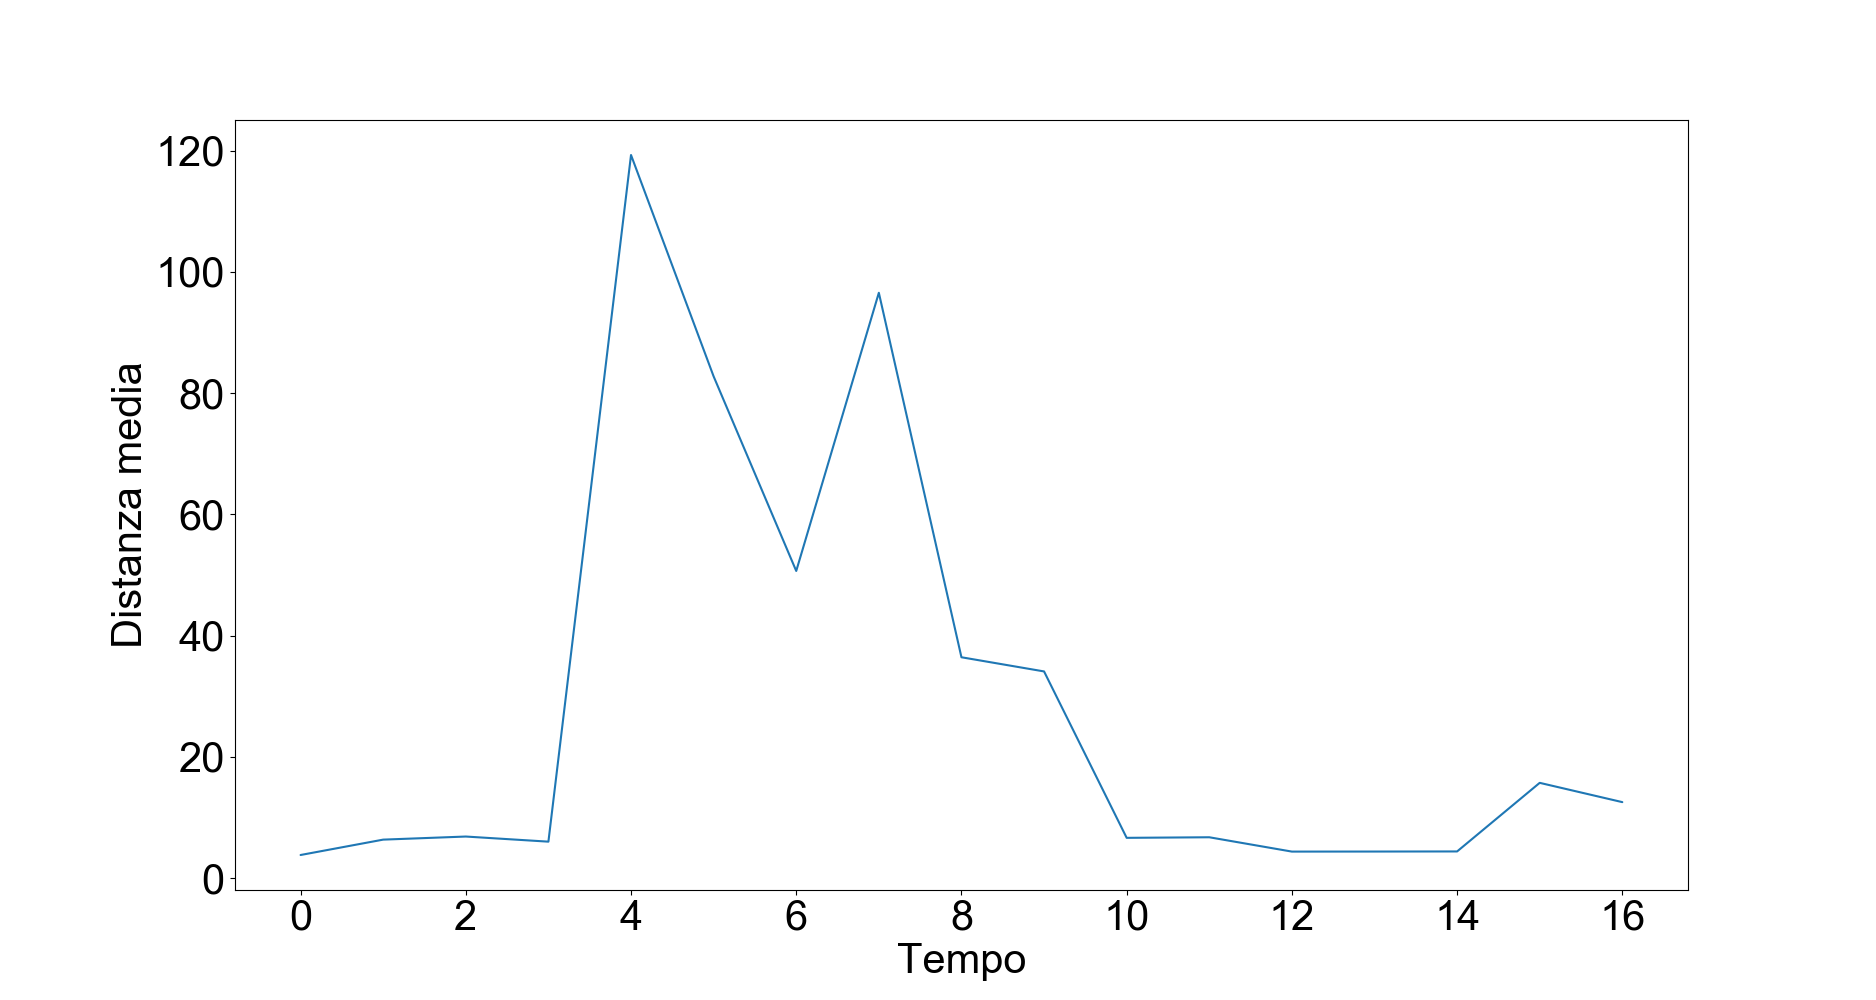
\includegraphics[width=0.8\textwidth]{DistanzaMedia.png}
    \caption{Variazione della distanza media tra i nodi nel grafo non orientato}
\end{figure}


Durante lo studio del grafo, è stato possibile identificare, per ogni periodo, i nodi più importanti della rete sulla base degli archi entranti e degli archi uscenti.
Questo ci ha dato un'idea di come gli account più importanti nella rete non siano variati troppo con il passare del tempo.

L'analisi dei nodi centrali in base agli archi entranti ha fornito delle informazioni interessanti, in particolare abbiamo notato che:
\begin{itemize}
    \item L'account che maggiormente rimane nella top 10 per ogni snapshot temporale è riconducibile all'Exchange ``Poloniex`` \cite{Poloniex}.
    Un exchange è un servizio che viene utilizzato per scambiare cripto valute con altre cripto valute o con monete tradizionali.
    Questo account è presente nella ``Top 10`` di tutti gli snapshot, ad eccezione dell'ultimo.
    Partendo dall'indirizzo di questo account e dal numero del blocco in cui termina ogni snapshot, siamo andati a recuperare dallo ``State Trie`` il ``balance`` di Poloniex, che mostriamo nella Figura 6.13.
    \begin{figure}[H]
    \centering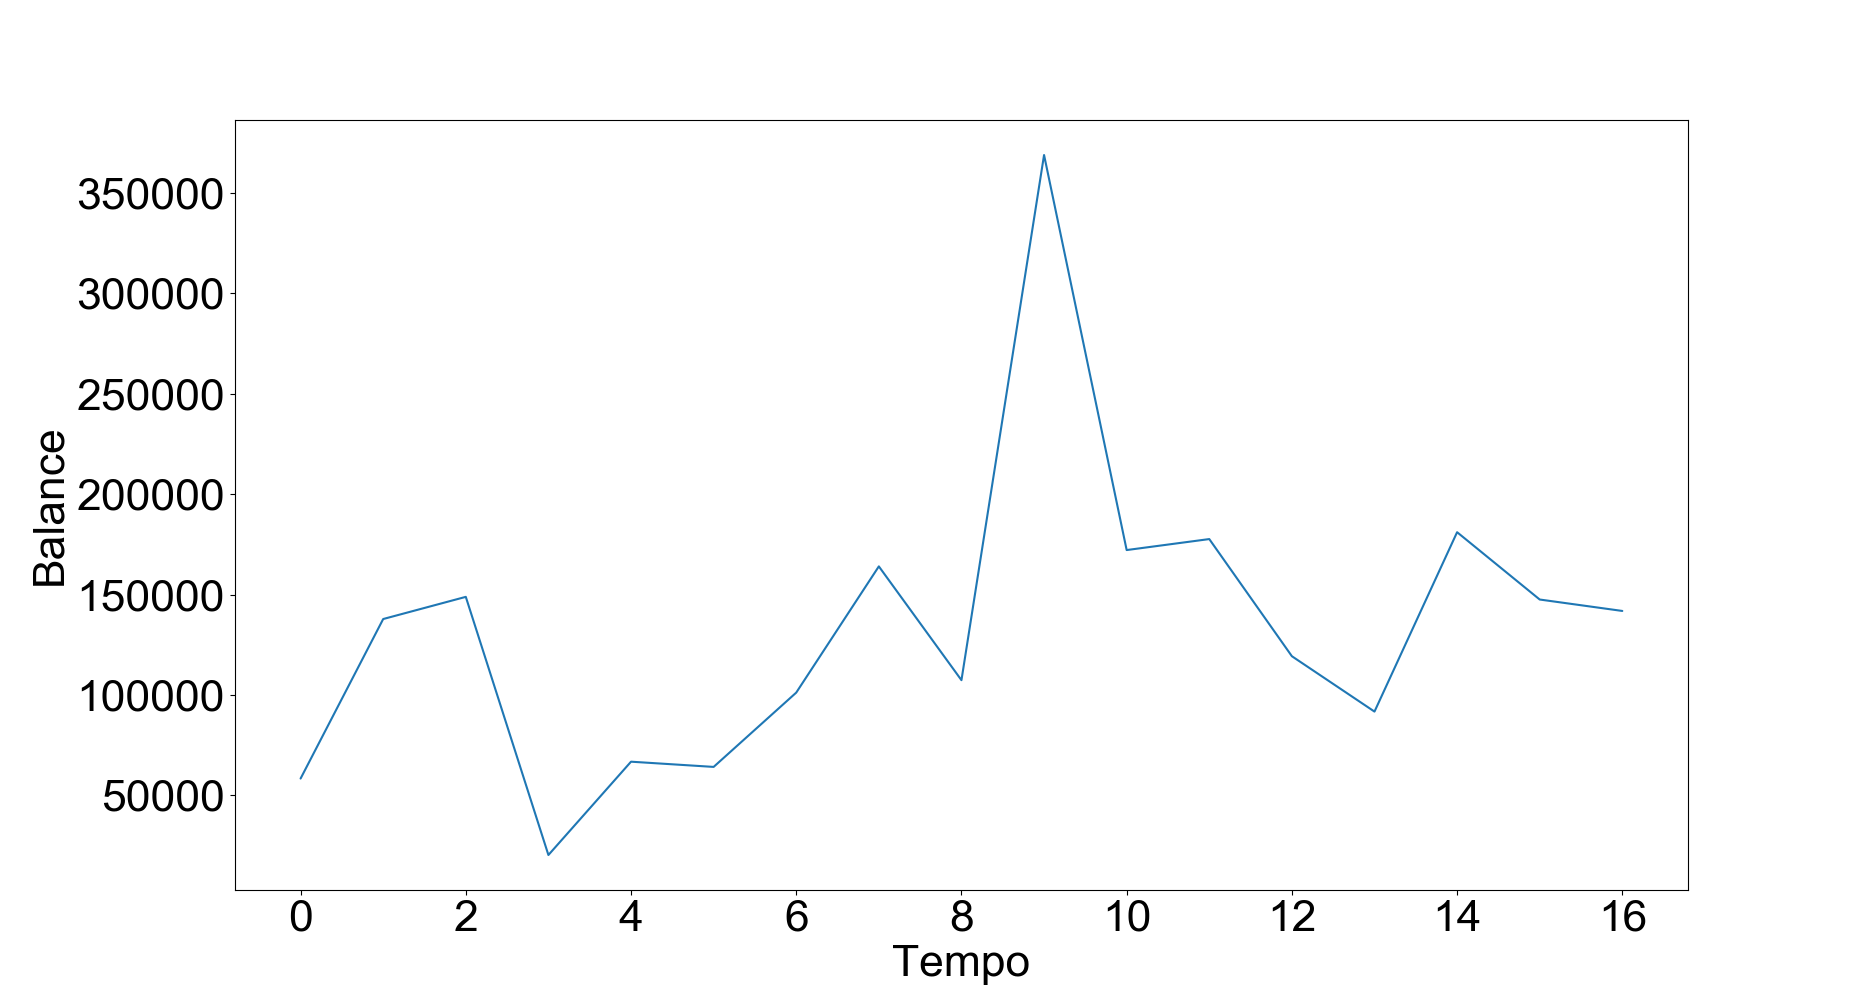
\includegraphics[width=0.9\textwidth]{Poloniex1.png}
    \caption{Balance in Ether dell'account Poloniex nel tempo}
    \end{figure}
    
    Un'osservazione particolarmente interessante è che nel momento in cui inizia la diminuzione del grado dell'account di questo exchange, in classifica compare un altro account, in questo caso un contratto, sempre relativo a Poloniex che nell'ultimo snapshot risulta il secondo in quanto a transazioni ricevute.
    
    \item Nelle classifiche ci sono vari account relativi a contratti che mantengono sempre un ``balance`` pari a 0 in tutti gli snapshot, uno di questi è relativo a Poloniex, l'exchange appena citato.
    
    \item Nei primi snapshot compare tra gli utenti più attivi un indirizzo relativo a ``Cryptsy``, questo scompare definitivamente dopo pochi snapshot, fatto osservato anche dal grafico dal suo balance nella figura 6.14:
    \begin{figure}[H]
    \centering\includegraphics[width=0.9\textwidth]{Cryptsy.png}
    \caption{Balance in Ether dell'account Cryptsy nel tempo}
    \end{figure}
    Da un'analisi di informazioni reperite in rete abbiamo scoperto che questo account ha subito, nel Luglio del 2014 (Snapshot 0), un attacco che ha portato al furto di circa 13.000 Bitcoin e 300.000 Litecoin corrispondenti a circa 6 milioni di dollari. Nel Gennaio 2016 (Snapshot 3) il servizio ha spiegato di essere stato hackerato e ha dichiarato fallimento.
    \item In classifica è presente anche un secondo exchange, di ShapeShift che ha addirittura due indirizzi.
    Un indirizzo di questo exchange è presente fin dal primo snapshot, possiamo vedere l'evoluzione del suo ``balance`` nella figura 6.15:
    
    \begin{figure}[H]
    \centering\includegraphics[width=0.9\textwidth]{Shapeshift1.png}
    \caption{Balance dell'account ShapeShift\textunderscore1 nel tempo}
    \end{figure}
    
    Il secondo indirizzo di ShapeShift compare per la prima volta nel sesto snapshot, anche in questo caso è stato creato un grafico per mostrare l'evoluzione del suo ``balance``.
    
    \begin{figure}[H]
    \centering\includegraphics[width=0.9\textwidth]{Shapeshift_2.png}
    \caption{Balance in Ether dell'account ShapeShift\textunderscore2 nel tempo}
    \end{figure}
    
    È interessante notare come nello snapshot 4 quando il balance del primo account decresce, aumenti invece il balance del secondo account appartenente a ShapeShift. Anche per il secondo account, abbiamo un picco della quantità di Ether posseduto e poi rapida dimizione di questo valore.
    
    Nella classifica ci sono anche altri due exchange particolarmente importanti, anche se compaiono meno rispetto ai primi di cui abbiamo parlato, si tratta di Kraken e di Bittrex.
    
    \item Tra gli account più attivi, in quanto a transazioni in entrata, abbiamo anche il contratto del ``The Dao``. Si tratta di una piattaforma nata nella blockchain di Ethereum che permette a qualsiasi startup di presentare il proprio progetto alla community del DAO e ricevere, nel caso in cui il progetto sia valido, dei finanziamenti. Per potere votare i progetti che vengono presentati è necessario possedere i ``Dao Token``, acquistabili utilizzando ether, nei mesi successivi al lancio il contratto del DAO ha ricevuto tantissime transazioni ed il successo è stato enorme.
    Anche per DAO abbiamo studiato la variazione del balance dell'account mostrando il risultato nella figura 6.17.
    \begin{figure}[H]
    \centering\includegraphics[width=0.9\textwidth]{TheDao.png}
    \caption{Balance in Ether dell'account The Dao nel tempo}
    \end{figure}
    
    E' interessante notare che l'account del ``The Dao`` ha avuto una crescita rapida del balance poco dopo la sua creazione, nello snapshot 6 corrispondente al periodo compreso tra Aprile e Giugno 2016. In questo periodo è stata raggiunta una quantità di Ether pari a circa 150 milioni di dollari. Si è poi verificata rapida diminuzione del balance tra Giugno e Luglio 2016.
    La motivazione di questa repentina variazione del balance è legata ad un attacco subito da questo account.
    L'attacco subito dal Dao ha comportato la perdita di circa 3.6 milioni di Ether, anche l'intero sistema di Ethereum ha avuto delle ripercussioni, nonostante il problema fosse di un singolo contratto e non di tutta la blockchain.
    Per cercare di risolvere i problemi di sicurezza sfruttati dall'hacker gli sviluppatori di Ethereum sono dovuti ricorrere ad un hard fork della blockchain il 20 Luglio del 2016.
    
\end{itemize}


\newpage
\section{Analisi svolte sul grafo diviso per tipo di transazione}

Il nostro dataset, grazie alla presenza di transazioni di tre tipi differenti si presta in modo abbastanza naturale ad una suddivisione in tre categorie:

\begin{itemize}
    \item Transazioni da utente esterno a utente esterno;
    \item Transazioni da utente esterno a contratto;
    \item Transazioni utilizzate per la creazione di un nuovo contratto.
\end{itemize}

Questa suddivisione ha messo in mostra che circa l'80\% delle transazioni sono effettuate da utenti esterni verso altri utenti, il 15\% sono da utenti a smart contract mentre solamente il 4\% circa sono state utilizzate per creare nuovi contratti.

\begin{figure}[H]
    \centering\includegraphics[width=\textwidth]{Torta.png}
    \caption{Divisione delle transazioni per tipo}
\end{figure}

\newpage
Su questi grafi suddivisi per tipo sono state svolte le medesime analisi del grafo completo, anche in questo caso iniziando dal numero di nodi e archi.

\begin{figure}[H]
    \centering\includegraphics[width=0.9\textwidth]{NumeroNodiTipo.png}
    \caption{Numero di nodi presenti in ognuno dei tre grafi}
\end{figure}


Avendo diviso il dataset in base al tipo di transazione abbiamo anche ritenuto utile cercare di capire quali fossero i nodi centrali in ognuno di questi grafi.
Per la parte di dati relativa alle transazioni destinate alla creazione di contratti sono stati identificati i seguenti 10 account che sono risultati essere i più attivi nel creare smart contracts.
Purtroppo, come si può notare dalla tabella 6.5, non sempre è stato possibile associare un nome all'indirizzo dell'account.

\begin{table}[H]
\centering
\begin{tabular}{ |c|c|c|} 
\hline
Indirizzo & Contratti creati & Nome \\
\hline
\multirow
0xb42b20ddbeabdc2a288be7ff847ff94fb48d2579 & 210984 & \\
0x42da8a05cb7ed9a43572b5ba1b8f82a0a6e263dc & 105582 & Yunbi_2\\
0x0536806df512d6cdde913cf95c9886f65b1d3462 & 25777 & Poloniex-GNT\\
0xab11204cfeaccffa63c2d23aef2ea9accdb0a0d5 & 17481 & Poloniex_2\\
0x3898d7580aa5b8ad8a56fcd7f7af690e97112419 & 15994 & \\
0x174443351e21d47ed9ab51517a301107d92ede64 & 11250 & \\
0xcf40d0d2b44f2b66e07cace1372ca42b73cf21a3 & 10689 & \\
0x48d466b7c0d32b61e8a82cd2bcf060f7c3f966df & 8843 & \\
0xd0d0fb67d2a37de67e1a794230bff37ee16737da & 7927 & Iconomi_2\\
0x86388554f35e69f078474b49174863238be7d58d & 6794 & \\
\hline 
\end{tabular}
\caption{Top 10 account in base alla creazione di contratti}
\end{table}


Per comprendere quanti contratti vengono creati da ogni utente abbiamo sfruttato la distribuzione del grado uscente ottenendo il grafico mostrato nella figura 6.20.

\begin{figure}[H]
    \centering\includegraphics[width=\textwidth]{DistribuzioneCreazioneContratti.png}
    \caption{Distribuzione del grado uscente dei nodi nel grafo con le sole transazioni di creazione dei contratti}
\end{figure}
Anche in questo caso si tratta di una power law, quindi una distribuzione standard dei dati.

Piuttosto interessante è anche la ``classifica`` dei top 10 per grado entrante calcolata sul grafo con le chiamate a contratti. Si tratta di un dato che rispecchia le analisi svolte in precedenza sugli account più attivi nella rete. La maggior parte degli account presenti nella tabella sono infatti riconducibili agli exchange.
\begin{table}[H]
\centering
\begin{tabular}{ |c|c|c|} 
\hline
Indirizzo & Chiamate & Nome \\
\hline
\multirow
0xe94b04a0fed112f3664e45adb2b8915693dd5ff3 & 143738 & Bittrex_2 \\
0xfa52274dd61e1643d2205169732f29114bc240b3 & 107762 & Kraken_5 \\
0x209c4784ab1e8183cf58ca33cb740efbf3fc18ef & 87302 & Poloniex_3 \\
0x86fa049857e0209aa7d9e616f7eb3b3b78ecfdb0 & 84275 & EOSTokenContract \\
0xa74476443119a942de498590fe1f2454d7d4ac0d & 70277 & Golem \\
0x7727e5113d1d161373623e5f49fd568b4f543a9e & 69510 & Bitfinex_2 \\
0xaa1a6e3e6ef20068f7f8d8c835d2d22fd5116444 & 66499 & ReplaySafeSplit \\
0x331d077518216c07c87f4f18ba64cd384c411f84 & 55276 & \\
0x8d12a197cb00d4747a1fe03395095ce2a5cc6819 & 41942 & EtherDelta_2 \\
0xbb9bc244d798123fde783fcc1c72d3bb8c189413 & 41469 & TheDAO \\
\hline 
\end{tabular}
\caption{Top 10 contratti per grado entrante}
\end{table}

Anche per il grafo con le sole chiamate a contratto è stata studiata la distribuzione del grado dei nodi, in particolare il grado entrante ci fornisce un'informazione per quel che riguarda la quantità di chiamate che vengono ricevute dai vari contratti.

\begin{figure}[H]
    \centering\includegraphics[width=0.9\textwidth]{DistribuzioneTransazioniVersoContratti.png}
    \caption{Distribuzione del grado entrante dei nodi nel grafo con le sole transazioni verso contratti}
\end{figure}


\newpage
\section{Analisi delle componenti connesse}



Utilizzando gli snapshot che avevamo a disposizione, abbiamo ritenuto utile analizzare anche le componenti connesse presenti all'interno dei vari grafi.
\newline
Con componente connessa di un grafo intendiamo il sottografo in cui ogni coppia di nodi è connessa da un cammino non orientato.
La prima analisi effettuata ci ha permesso di capire, per ogni snapshot, la percentuale di nodi che sono presenti all'interno della componente connessa più grande del grafo $G^T$.
\newline
Il calcolo di questa percentuale è stato svolto utilizzando la seguente formula:

\begin{equation}
    N^T = \frac{|C^T|}{|V^T|}
\end{equation}

dove con $|C^T|$ indichiamo il numero di nodi contenuti nella componente connessa più grande, con $|V^T|$ il numero di nodi contenuti nel grafo al tempo T e con $N^T$ il valore calcolato.

Nella Figura 6.23 viene mostrato il risultato ottenuto, è possibile notare come la frazione di nodi presenti all'interno della componente connessa più grande sia sempre molto alta, ovvero contiene più del 90\% di nodi del grafo.

\begin{figure}[H]
    \centering\includegraphics[width=0.9\textwidth]{GiantCC.png}
    \caption{Frazione di nodi nella componente connessa più grande}
\end{figure}

Il secondo risultato  è speculare al primo, in questo caso abbiamo considerato per ogni snapshot la percentuale di nodi che non sono presenti all'interno della componente connessa più grande di ogni snapshot.
\newline
In questo caso la formula utilizzata per il calcolo del valore in ogni snapshot è la seguente:

\begin{equation}
    S^T = \frac{|V^T| - |C^T|}{|V^T|}
\end{equation}

\newline
Come possiamo vedere, il grafico è speculare rispetto a quello della Figura 6.23

\begin{figure}[H]
    \centering\includegraphics[width=0.9\textwidth]{GiantCCSpeculare.png}
    \caption{Frazione di nodi esterni alla componente connessa più grande}
\end{figure}

\chapter{Conclusioni}

Questo tirocinio, svolto nel periodo compreso tra Luglio e Settembre 2018, ha arricchito il mio bagaglio culturale permettendomi l'avvicinamento al mondo della blockchain e in particolare al protocollo Ethereum.
L'obiettivo è stato quello di parsare le informazioni contenute nella blockchain di Ethereum per poi rappresentare i dati ottenuti in un grafo e svolgere delle analisi.

La conoscenza ottenuta durante il tirocinio spazia dalla teoria alla pratica.
\newline
Dal punto teorico è stato fondamentale lo studio del White Paper e dello Yellow Paper di Ethereum. Questi due documenti hanno permesso di comprendere a fondo la struttura di blocchi, transazioni e receipt.
La conoscenza di queste informazioni teoriche si è rivelata necessaria quando siamo passati alla parte pratica del lavoro che prevedeva la scrittura di un parser del contenuto della blockchain. A tale scopo abbiamo implmentato due soluzioni, la prima ha richiesto lo sviluppo di un parser in Java, la seconda l'utilizzo del client Geth.
La parte del tirocinio che ho trovato più interessante e che mi ha maggiormente appassionato è stata quella relativa alla costruzione e all'analisi del grafo.
In quest'ultima fase, per l'analisi del grafo, ho utilizzato WebGraph che mi ha permesso di avvicinarmi al campo delle analisi dei grafi.

L'analisi è stata svolta su vari grafi, inizialmente su quello contenente tutte le transazioni.
In questa prima fase è stato possibile conoscere alcune informazioni relative al grafo come il numero di nodi e archi contenuti al suo interno, la distanza media tra i nodi e il diametro. Proprio quest'ultimo ha attirato la nostra attenzione a causa del valore piuttosto elevato e ci ha portato a ipotizzare che alcuni cammini artificiali e anomali all'interno del grafo possano averne influenzato la lunghezza.
Successivamente il dataset è stato suddiviso in base al timestamp dei blocchi permettendo lo svolgimento di un'analisi temporale su 17 snapshot.
Queste analisi ci hanno mostrato la crescita di nodi e archi all'interno del grafo nel corso del tempo. La crescita è stata anche messa in relazione alla variazione del valore dell'Ether che ha subito un aumento nello stesso periodo in cui sono aumentate transazioni e nodi nella rete.
È stata studiata anche la variazione della dimensione della componente connessa più grande, questa analisi ci ha mostrato che più del 90\% dei nodi fanno parte di questo sottografo.
Piuttosto interessante è stato anche lo studio della centralità, questo ci ha fornito, per ogni snapshot, l'elenco dei nodi più importanti nella rete. È stata quindi eseguita una ricerca per comprendere il più possibile la storia di questi nodi e l'evoluzione del loro balance.
\newline Le ultime analisi sono state svolte suddividendo il dataset in base al tipo delle transazioni. In particolare abbiamo trovato interessanti i risultati legati allo studio della distribuzione del grado entrante nel grafo con le sole transazioni verso i contratti e la relativa ``Top 10`` degli smart contract più chiamati dagli utenti.
Un'analisi simile è stata svolta nel grafo con le sole transazioni di creazione dei contratti, in questo caso abbiamo ottenuto la distribuzione del grado uscente e la ``Top 10`` degli utenti che hanno creato più contratti.

A causa dell'alta potenza computazionale richiesta non è stato possibile ottenere tutti i dati ad oggi presenti nella blockchain di Ethereum e come indicato nella sezione 5.1, l'analisi è stata svolta solamente su una porzione delle transazioni.
\newline 
Uno degli obiettivi per il futuro è quello di estrarre i blocchi rimanenti, corrispondenti alle transazioni avvenute nell'ultimo anno e svolgere anche su quelli lo stesso lavoro descritto in questa relazione.
L'analisi di tutti i dati andrebbe a fornire un quadro completo della blockchain di Ethereum, dalla nascita fino ai giorni nostri.

Un altro sviluppo possibile di questo tirocinio riguarda lo studio della proprietà ``Rich get Richer`` ovvero l'analisi dell'accumulo di ricchezza in alcuni account dell'ecosistema di Ethereum.


\chapter{Ringraziamenti}

Un particolare ringraziamento va ai relatori, prof.ssa Laura Ricci e dott. Damiano Di Francesco Maesa che si sono sempre dimostrati disponibili e mi hanno seguito assiduamente durante questo percorso fornendomi consigli utili al raggiungimento del mio obiettivo.
\newline 
Vorrei poi ringraziare anche il Dott. Andrea Marino che durante il tirocinio è stato consultato più volte per avere spiegazioni e consigli riguardo alla creazione e all'analisi del grafo delle transazioni.

\appendix


\bibliographystyle{unsrt}
\bibliography{references}

\end{document}